\documentclass[twocolumn,superscriptaddress,aps]{revtex4-1}

\usepackage[utf8]{inputenc}

\usepackage{amsfonts}
\usepackage{amssymb}
\usepackage{amsmath}
\usepackage{amsthm}
\usepackage{url}
\usepackage[colorlinks=true, allcolors=blue]{hyperref}
\usepackage{bbold}
\usepackage{bm}
\usepackage{graphicx}
\usepackage{color}
\usepackage{subcaption}
\usepackage{float}
\usepackage{wrapfig}
\usepackage{svg}
\usepackage{enumitem}

\begin{document}


% ==============================================================================

\title{\Large{INFO8010: Scene Classification}}
\vspace{1cm}
\author{\small{\bf HOGGE Louis}}
\affiliation{\texttt{louis.hogge@student.uliege.be} (\texttt{s192814})}
\author{\small{\bf VANDERHEYDEN Julien}}
\affiliation{\texttt{julien.vanderheyden@student.uliege.be} (\texttt{s203734})}
\author{\small{\bf WEBER Tom}}
\affiliation{\texttt{t.weber@student.uliege.be} (\texttt{s203806})}

\maketitle

% ==============================================================================

\section{Introduction}

The rapid advancements in robotics are ushering in a new era where robots are poised to seamlessly integrate into our daily lives, undertaking a myriad of tasks in diverse and dynamic environments. As robots transition from the confines of industrial settings to the bustling landscapes of our homes, streets, and workplaces, a fundamental question arises: How can we equip these robots with the adaptability and flexibility to navigate and thrive in such complex and ever-changing surroundings? How can we develop models that transcend specific applications, enabling robots to effortlessly transition between tasks without the need for extensive reconfiguration?

At the heart of this quest lies the concept of \textbf{Scene Understanding}—a critical component in endowing robots with the cognitive ability to comprehend and respond to their environmental context. Scene Understanding, in the context of this project, entails the capacity to discern the nature of the environment in which an agent operates, based on visual inputs such as images or videos.

While robotics stands as a prominent application domain for Scene Understanding, our focus is to address the problem in a general way, by identifying various environments related to daily life, which could then be applied to other applications such as aiding blind people.

Scene Understanding, being a multifaceted problem, encompasses various sub-tasks including scene classification, object detection, scene retrieval, and more. In this project, our focus is directed towards the specific task of \textbf{Scene Classification}. Scene Classification involves associating an image of the environment with a label from a predefined set of categories, which seemed to us to be the task we were best equipped for.


\section{Related Work}

Since scene classification is just a particular case of image classification, significant work has already been done in this field from the introduction of Convolutional Network by Yann Lecun in 1998 \cite{lecun_cnn} . So numerous particular models have been presented since this time, almost all being based on the classical convolutional architecture. It has been decided decided to stick  to the most famous and state-of-the-art ones which will be presented in this section. \\

A first standard and famous architecture is VGG (Visual Geometry Group) introduced by \textit{Simonyan and Zisserman} \cite{vgg}, which implements a classical serie of blocks composed of 2 convolutional layers with 3x3 kernels followed by a pooling layer, the whole serie being followed by a full connected layer and a softmax layer. The particularity of this architecture is its depth, going from 16 to 19 layers, which is feasible thanks to the use of minimum-size kernels. \\

The biggest limitation to increasing the depth of the models was the problem of vanishing/exploding gradients. A solution to this problem has been brought in 2015 by \textit{Kaiming He et. al.} \cite{resnet}, which consists in adding skip connections between the differents blocks, in such a way that the different gradients are now able to travel through the network without vanishing. \\

Another very famous convolutional neural network architecture is the DenseNet, introduced in 2017 by \textit{Gao Huang et al.} \cite{denset}. The specificity of this architecture is the addition of connections between all layers : the output of each layer is given as input to all the following layers. \\

Finally, a popular architecture that deviates significantly from convolutional networks is the transformer. This architecture allows the processing of sequences that can be used as well for both classification and generation. The link to image classification was established in 2021 by \textit{Dosovitskiy et al} \cite{vit}, proposing to treat an image as a sequence of smaller patches and use a transformer to classify it. \\

\section{Methods}

As explained in the previous section, several state-of-the-art architectures have been implemented and will be presented in details in this section. 

\subsection{ConvNet}

A convolutional network is generically defined as a composition of convolutional layers, pooling layers, linear rectifiers and fully connected layers.

\subsubsection{Common structure}

\begin{figure}[H]
    \centering
    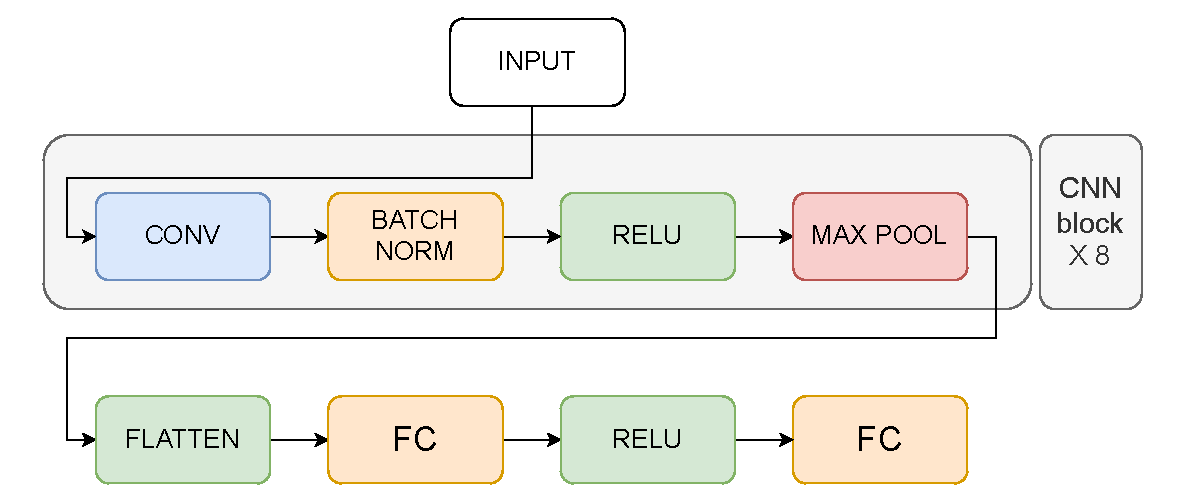
\includegraphics[width=0.85\linewidth]{images/cnn.pdf}
    \caption{ConvNet architecture}
    \label{fig:cnn_arch}
\end{figure}

\subsubsection{Input}
The input is a 256x256 image, every image in a digital device being stored as a matrix of pixel values. This is referred to as a channel, a certain component of an image. Now, with a typical digital camera, every image will have three channels, red, green, and blue (RGB) which can be imagined as three 2D matrices stacked upon one another.

\begin{figure}[H]
    \centering
    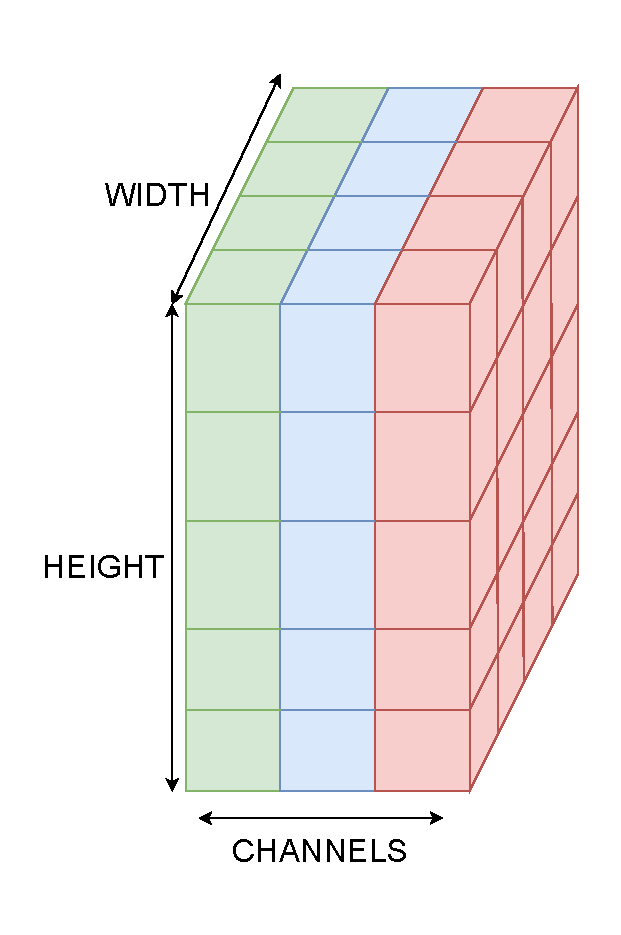
\includegraphics[width=0.5\linewidth]{images/input_image.pdf}
    \caption{Input image}
    \label{fig:enter-label}
\end{figure}

\subsubsection{Convolutionnal layer}

In CNNs, the convolution operator is  implemented thanks to a feature detector/filter/kernel (same thing), represented as a matrix of smaller dimension than the input. The convolutional operation is made by moving the kernel across the input image, taking the dot product of the matrices and saving the result in a third matrix, called the feature map of the original image.

\begin{figure}[H]
    \centering
        \begin{subfigure}[t]{.3\textwidth}
        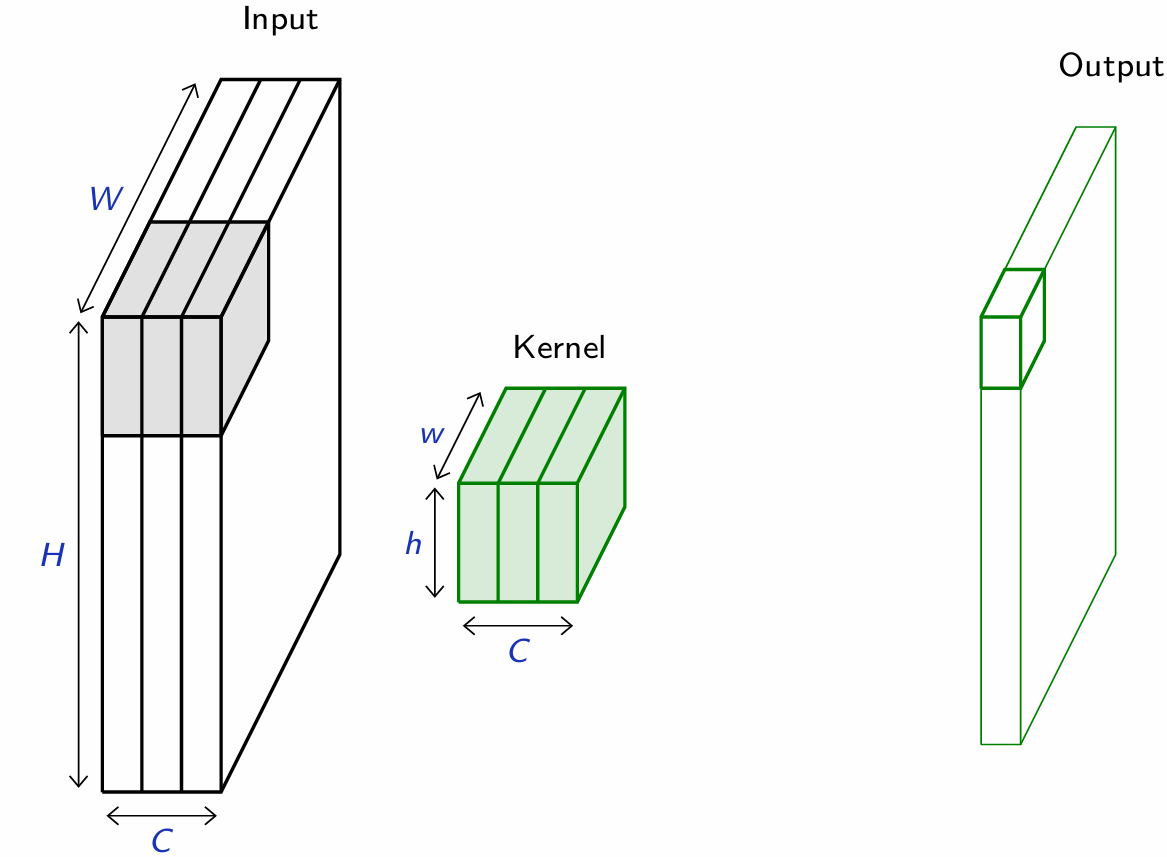
\includegraphics[width =\textwidth]{images/kernle_mov1.png}
        \caption{Moving kernel at step 0}
        \label{fig:kernel_mov1}
        \end{subfigure}
            \hfill
        \begin{subfigure}[t]{.3\textwidth}
        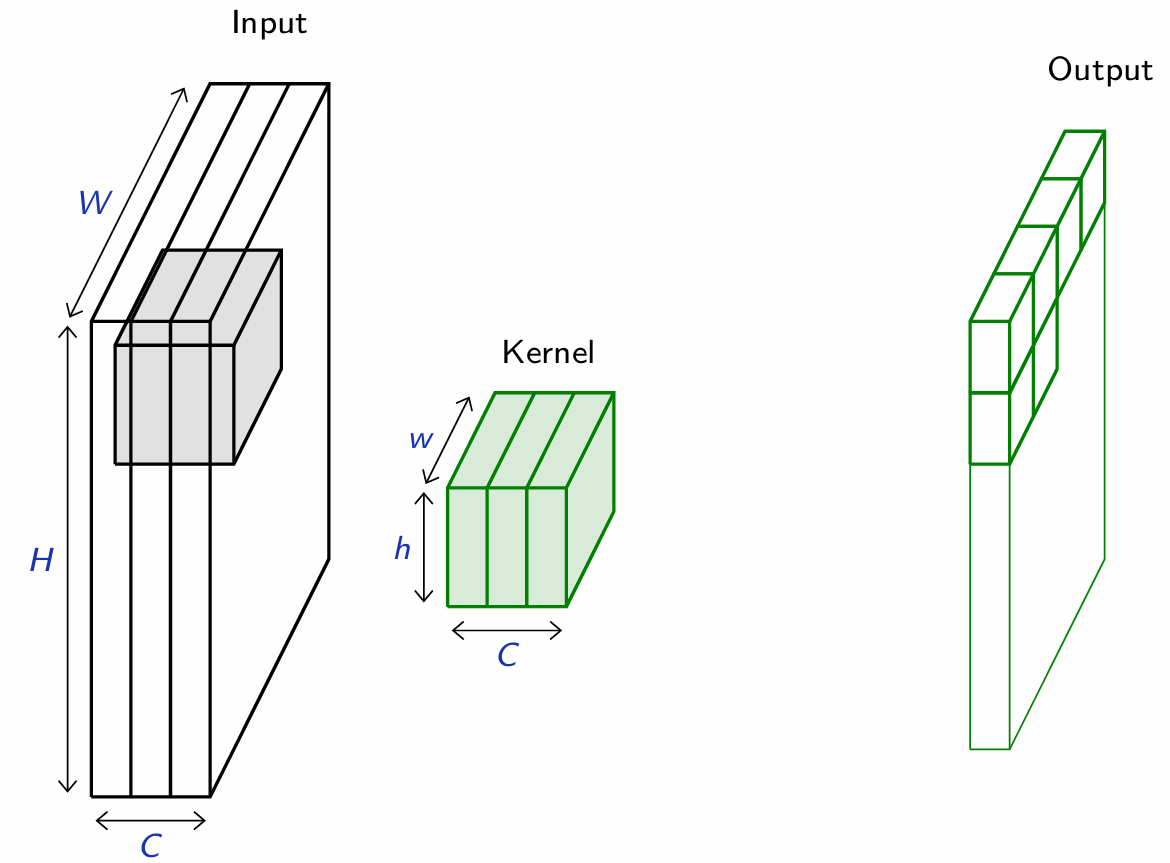
\includegraphics[width =\textwidth]{images/kernel_move2.png}
        \caption{Moving kernel at step 6}
        \label{fig:kernel_mov2}
        \end{subfigure}
            \hfill
        \begin{subfigure}[t]{.3\textwidth}
        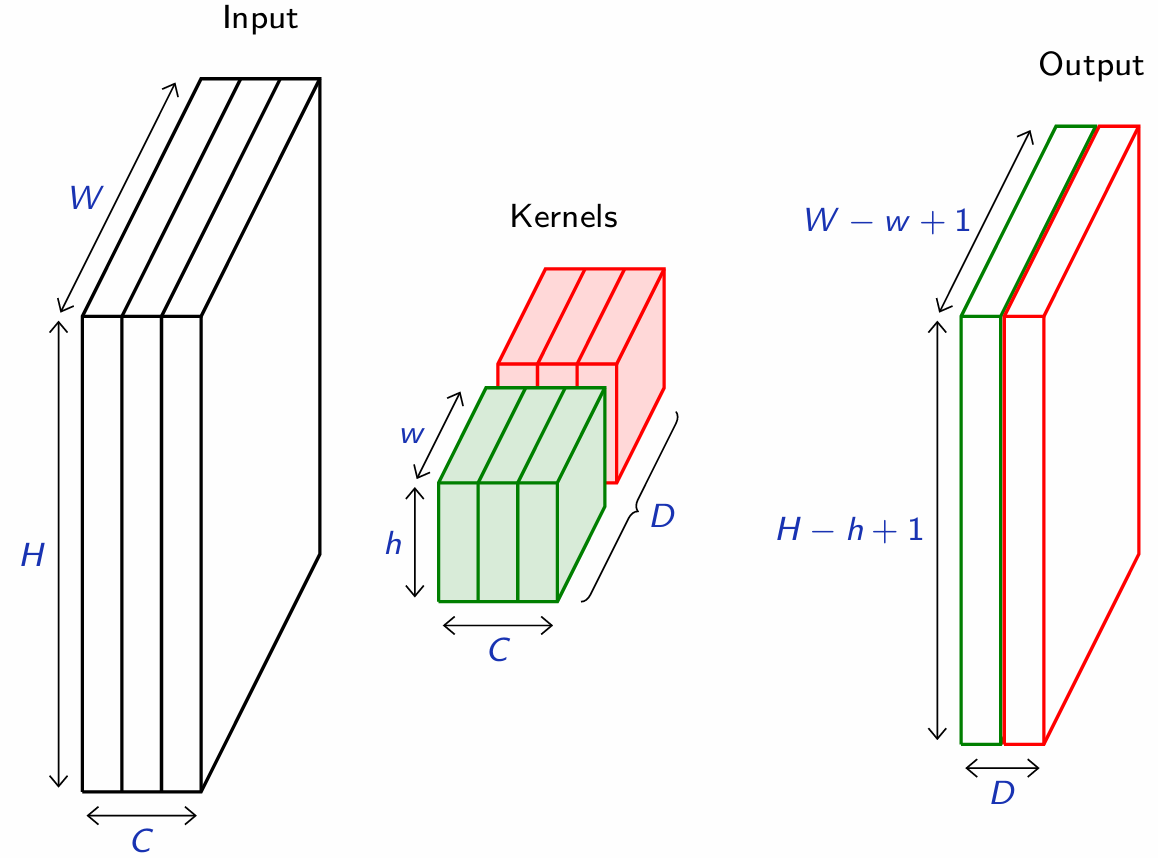
\includegraphics[width =\textwidth]{images/kernel_move3.png}
        \caption{Multiple kernels for image with 2 channels}
        \label{fig:kernel_mov3}
        \end{subfigure}
    \caption{Illustration of moving kernel to produce a convolutionnal layer from \href{https://fleuret.org/dlc/materials/dlc-slides-4-4-convolutions.pdf}{François Fleuret's course}}
    \label{fig:1.2}
\end{figure}

This feature matrix allows the network to detect edges, corners, simple shapes and patterns. Notice that each CNN block start with a certain number of kernels (here 16 of size 3x3) and is doubled in the next one. For each of the convoluted pixels in the feature map, a ReLU activation function is applied to introduce non-linearity, which helps the network to learn complex patterns. 

\subsubsection{Batch normalization}

This layer is not make part of the generic CNN architecture but they offer some benefits in efficiency and robustness.

\\

By normalizing the inputs of each layer to have a consistent mean and variance, batch normalization mitigates issues related to internal covariate shift, where the distribution of inputs to layers changes during training. This stabilization of the learning process enables the use of higher learning rates, accelerates convergence, and often leads to improved model performance.

\\

 Additionally, batch normalization acts as a form of regularization, reducing the need for other regularization methods like dropout. Consequently, it can enhance the generalization capability of the model, resulting in better accuracy on unseen data.

\subsubsection{Pooling layer}

Pooling layers are used to downsample the feature maps, keeping the most important parts and discarding the rest, what is primarily done to reduce the overfitting rate, so that calculations can be sped up in later layers due to the reduced spatial size of the image. The type of pooling implemented in convolutional network is max pooling, in which another kernel is taken and slided across the input feature maps. The largest pixel value in that region is finally saved in a new output feature map.

As can be seen on Fig. \ref{fig:max_pool_visual}(number classifier), the max pooled layer still retains the important information from the convolutional layer, while being smaller in spatial size.

\begin{figure}[H]
    \centering
    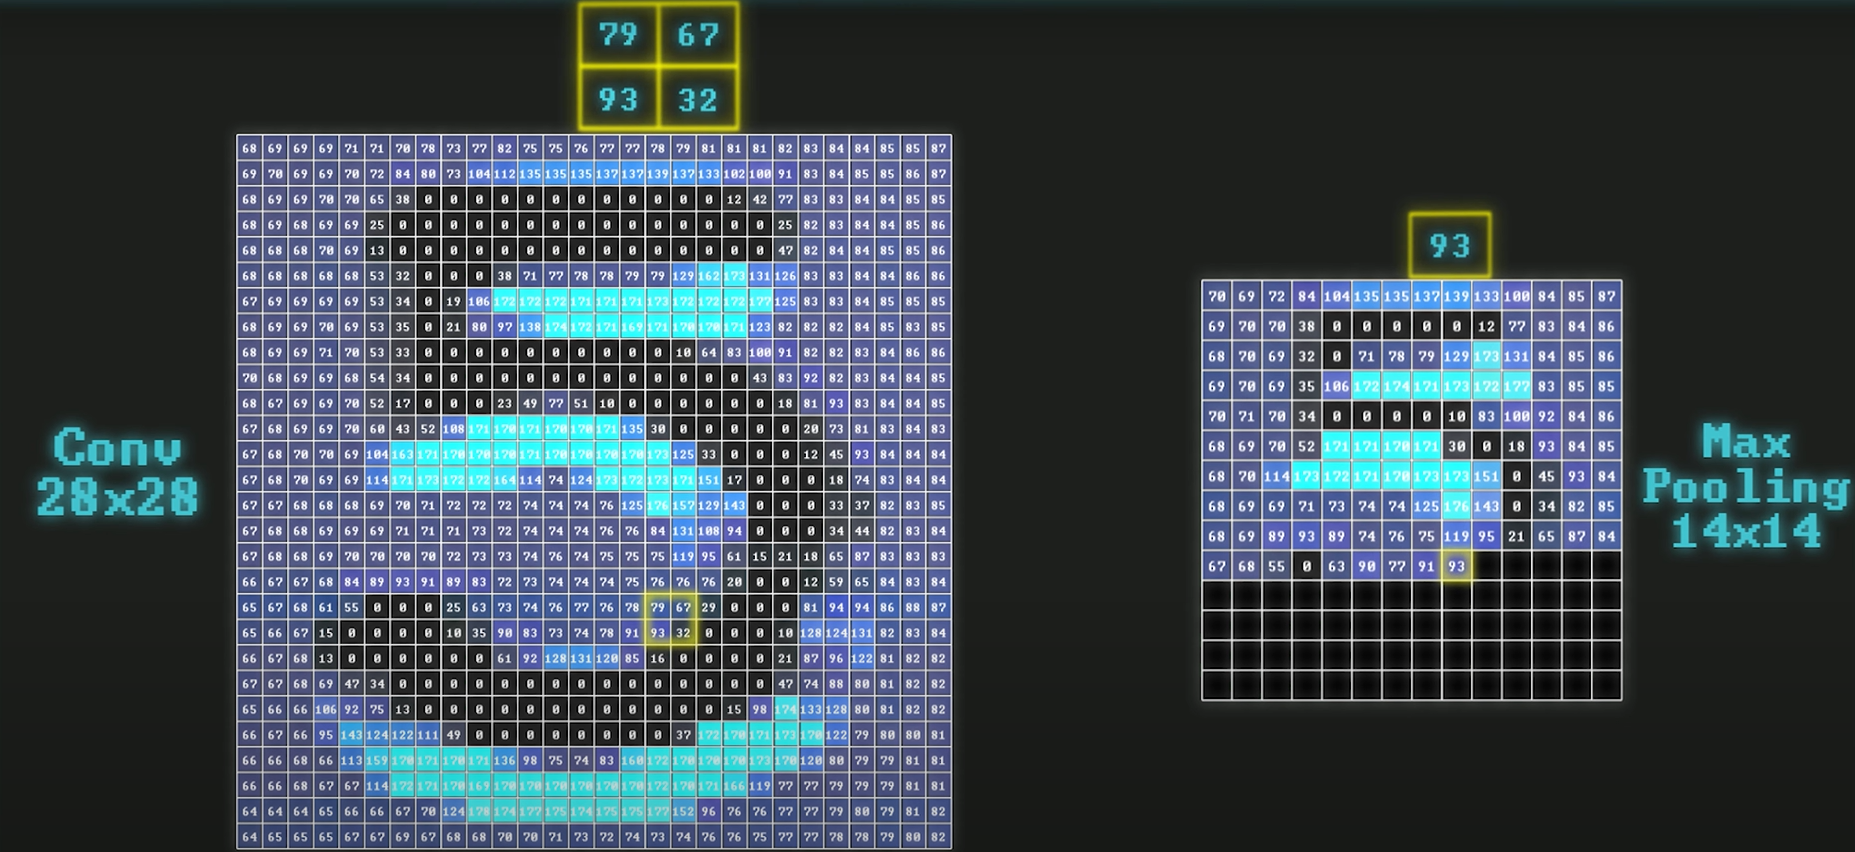
\includegraphics[width=1\linewidth]{images/max_pool_visual.png}
    \caption{Visual representation of max pooling for number classification from \href{https://www.youtube.com/@OptimisticFuturology}{youtube}}
    \label{fig:max_pool_visual}
\end{figure}

Those layers are then repeated to build up more abstract representation in the network, to detect high level features with lowest possible spatial resolution : this is the network's feature extraction part.

\subsubsection{Hyper-parameters}
\begin{enumerate}
    \item 
    \textbf{Kernel size:} It has been decided to use 3 for convolutionnal layer and 2 for max pooling. Smaller kernels have smaller receptive field, meaning they capture fine, detailed features such as edges and small textures(to capture larger patterns, multiple convolutional layers are needed, effectively increasing the receptive field). The advantage of small kernels is their small computational cost due to the smaller number of parameters.
    \item 
    \textbf{Stride:} The step size with which the filter moves across the image. A stride of 1 means the filter moves one pixel at a time. In our project, it is set to 2 for each max pooling layer.
    \item 
    \textbf{Padding:} Consist in adding extra pixels around the input image to control the spatial size of the output. "Same" padding keeps the output size the same as the input, while "valid" padding reduces it. It has been set to 2 for each max pooling layer and convolutionnal layer.
\end{enumerate}

\subsubsection{Classifier}

The classsifier is represented by the second row on Fig.~\ref{fig:cnn_arch}.

This part is composed of fully connected layers, similar to a feedforward network except that the input of these perceptron layers are the high level abstracted features deducted by the convolutional layers, rather than the raw input pixels.

In the implemented architecture, dimensions are as follows:

\begin{align*}  
input\_size  = nb\_kernels & * 2^{\text{nb CNNs blocks} - 1} \\ & * \frac{H}{2^\text{nb CNNs blocks}} \\ & * \frac{W}{2^\text{nb CNNs blocks}}
\end{align*}

\begin{itemize}
    \item 
    nb CNNs blocks = 8, according to the architecture on Figure~\ref{fig:cnn_arch}.
    \item 
    nb\_kernels = 16, is the number of kernels/filters used for the first CNN block in grey on Figure~\ref{fig:cnn_arch}
    \item 
    H = height of the image (pixels), W = width of the image (pixels).
\end{itemize}

\subsection{ResNet}

\subsubsection{General Idea}
The ResNet builds on the previous network by adding a key feature: \textbf{the skip connection}. A skip connection simply adds the input of a layer or a block of layers to the output of that layer/block. This residual connection helps the network avoid the gradient vanishing problem, allowing for the construction of deeper networks.

\begin{figure}[hbtp]
    \centering
    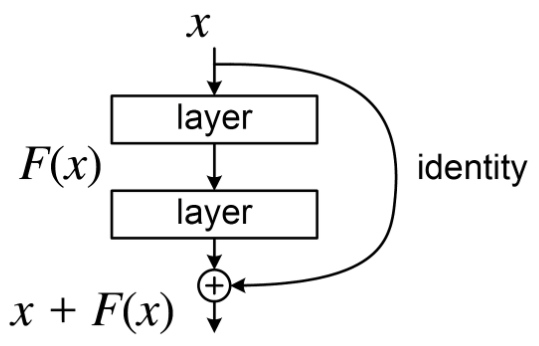
\includegraphics[width = 0.25 \textwidth]{images/skip_connection.png}
    \caption{The skip connection}
    \label{fig:skip_connection}
\end{figure}

\subsubsection{Practical Implementation : Layers}

In \cite{resnet}, a general architecture of 4 high-level layers is outlined, with the size adaptable to available computing resources. Given the limited computing resources for this project, it has been chosen to implement the lighter version of ResNet known as \textbf{ResNet18}. \\

Each layer in ResNet consists of several residual blocks that implement skip connections, with the number of blocks varying based on the model size. For ResNet18, each layer has 2 residual blocks. The first block in each layer reduces the image size by half using striding, while the subsequent blocks maintain the same dimensions. This results in a total reduction of 
$2^4 = 16$, progressively increasing the network's receptive field. \\

These four residual layers are preceded by a standard convolution layer that adjusts the input to the desired dimensions. After passing through the 4 ResNet layers, the output is fed into a classifier consisting of an average pooling layer, a dropout layer, and a linear layer.\\

\subsubsection{Practical Implementation : Residual Block}

The core of the architecture is the residual block, which effectively implements the skip connection. Each block consists of two 3x3 convolutional layers, each followed by batch normalization and a ReLU activation function. The skip connection is added just before the second ReLU, effectively skipping the two convolutional layers.\\
The first layer may optionally change the dimensions through striding. When this happens, the skip connection must also adjust the dimensions to match : this is achieved by passing the input through a convolutional layer with striding, followed by a batch normalization layer. The standard residual block without dimension adaptation is illustrated on Fig. \ref{fig:residual_block}. 
\begin{figure}[hbtp]
    \centering
    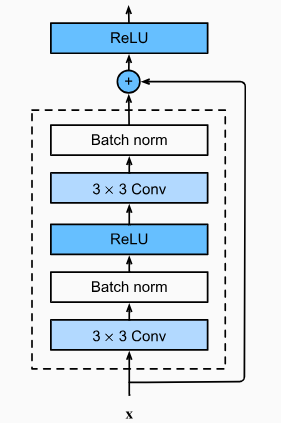
\includegraphics[width = 0.25 \textwidth]{images/residual_block.png}
    \caption{Standard Residual Block}
    \label{fig:residual_block}
\end{figure}


\subsection{DenseNet}

DenseNet also builds on the previous ConvNet by adding its unique feature of dense connectivity between layers: each layer receives inputs from all preceding layers and transmits its own feature maps to all subsequent layers. This architecture facilitates feature reuse, strengthens feature propagation, reduces the number of parameters and alleviates the problem of the vanishing gradient\cite{denset}.

\subsubsection{Dense Connectivity}

In a DenseNet, each layer is connected to every other layer in a feed-forward fashion. If there are $L$ layers in the network, there are $\frac{L(L+1)}{2}$ direct connections. For each layer $l$ the feature maps of all preceding layers $\{x_0, x_1, ..., x_{l-1}\}$ are used as inputs, and its own feature map $x_l$ is passed on to all subsequent layers. This dense connectivity pattern is illustrated as follows:
$$x_l = H_l([x_0, x_1, ..., x_{l-1}])$$

where $[x_0, x_1, ..., x_{l-1}]$  refers to the concatenation of the feature maps produced by layers $0, 1, ..., l-1$, and $H_l$ denotes the composite function of operations (such as Batch Normalization, ReLU, Convolution) applied at the $l$-th layer.

\subsubsection{Dense Block}

The DenseNet is composed of several dense blocks, each consisting of several convolutional layers where the above-mentioned dense connectivity is applied. Within each dense block, to reduce the number of parameters, a bottleneck layer is introduced. This consists of a 1×1 convolution layer that is implemented before each 3×3 convolution. This bottleneck layer allows for a reduction in feature maps and an improvement in computational efficiency.

Each dense block can be represented as:

$$[H_0(x_0), H_1(x_0, x_1), ... H_{L-1}([x_0, x_1, ..., x_{L-2}])]$$

Between these blocks, transition layers are used to perform down-sampling, reducing the spatial dimensions of the feature maps while controlling the complexity of the model. The transition layers include a 1×1 convolutional layer followed by a 2×2 average pooling layer.

\begin{figure}[hbtp]
    \centering
    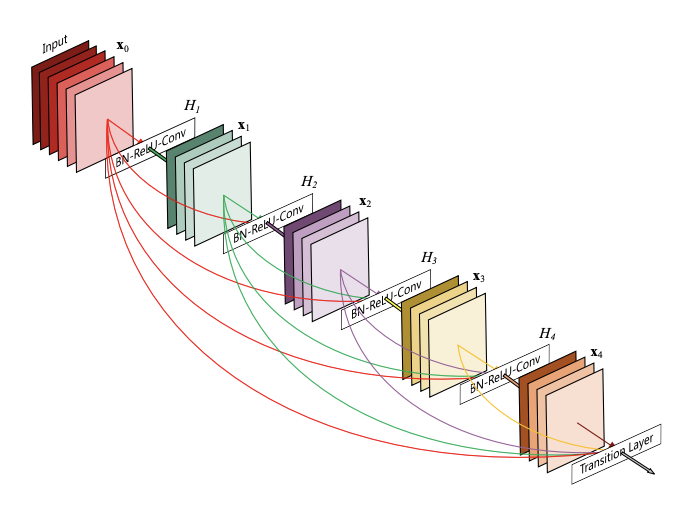
\includegraphics[width = 0.3 \textwidth]{images/dense_block.png}
    \caption{5-layer dense block with a growth rate of $k=4$ \href{https://pytorch.org/hub/pytorch_vision_densenet/?fbclid=IwZXh0bgNhZW0CMTAAAR2QMv_xnytuuHmi7n34mhoB6XCRXNTiO3u_fmpqeSZaPDUBdR6R2FNBUYs_aem_AbJUZaQWuj1e5Ljq4fDnHdOomyKn37ecNYOHxxY7p05yRNH6rG_MAFDLYep3f6NVew4tn8zNwhHHC5uCMY9ibzLE}{pytorch doc}}
    \label{fig:dense_block}
\end{figure}

\subsubsection{Growth Rate}

The growth rate $k$ in DenseNet is a critical hyper-parameter that controls the number of feature maps produced by each layer. Specifically, if the function $H()$ produces $k$ feature maps, then at layer $l$, the number of input feature maps becomes $k_0 + k(l-1)$, where $k_0$ is the number of channels in the input layer. This lower growth rate is due to the fact that each layer has access to the feature maps of all previous layers, making it representative of the overall state of the network. This extended access allows each layer to contribute new information without having to relearn the representations, thus improving efficiency and reducing redundancy.

\subsubsection{Implementation}

DenseNet is implemented with different configurations, such as DenseNet-121, DenseNet-169, DenseNet-201 and DenseNet-264, where the numbers refer to the total number of layers in the network.

In this project, a much smaller DenseNet has been implemented to accommodate computational power limitations.

\subsection{Visual Transformer (ViT)}

\subsubsection{Patchification}

The visual transformer is based on the principle of all transformers : it processes sequences. So, the images are transformed into sequences through an operation called \textit{patchification}. It consists in dividing the images (assumed to be square) into smaller images and process them sequentially. This process is dictated by a hyper-parameter \textit{n\_patches} that governs in how much patches each dimension is divided. Images of shape (32,32) with \textit{n\_patches} equal to 8 will so be divided into \textit{n\_patches²} = 64 patches of dimensions (32/\textit{n\_patches}, 32/\textit{n\_patches}) = (4,4). This process is illustrated on Fig. \ref{fig:patchify}.

\begin{figure}[hbtp]
    \centering
    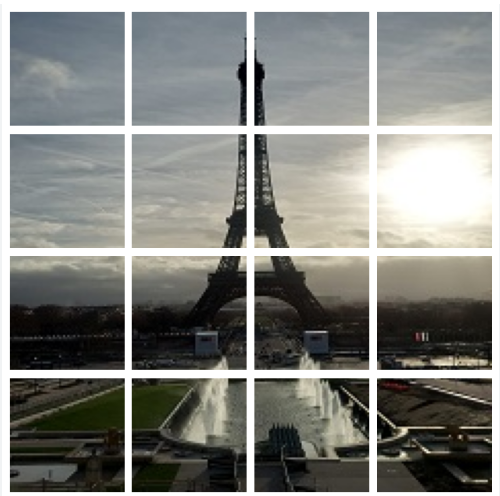
\includegraphics[width = 0.25 \textwidth]{images/patchify.png}
    \caption{Patchification with \textit{n\_patches} = 4}
    \label{fig:patchify}
\end{figure}

\subsubsection{Embedding}

Once the images are transformed into sequences, the next step is to perform \textit{Embedding} to move them in a lower dimensional space of dimensions \textit{n\_embedding}, \textit{n\_embedding} being an other crucial hyper-parameter. But two things have to be noticed : 

\begin{itemize}
    \item Since the problem considered is classification and not sequence generation, a \textit{classification token} should be added. The value of this token after going through the network will produce the final prediction. 
    \item As in every transformers, the network should also be aware of the relative position of the different patches in the sequence. This operation is called \textit{positional embedding} and  can be done in different way. The "classic" way is to add a particular combination of sine and cosine taking as argument the position of the considered $i^{th}$ token to $j^{th}$ coordinate. 

    
\[
p_{i,j} = 
\begin{cases} 
\sin \left( \frac{i}{10000^{\frac{j}{d_{\text{emb-dim}}}}} \right) & \text{if } j \text{ is even} \\
\cos \left( \frac{i}{10000^{\frac{j-1}{d_{\text{emb-dim}}}}} \right) & \text{if } j \text{ is odd}
\end{cases}
\]
    \begin{figure}[H]
        \centering
        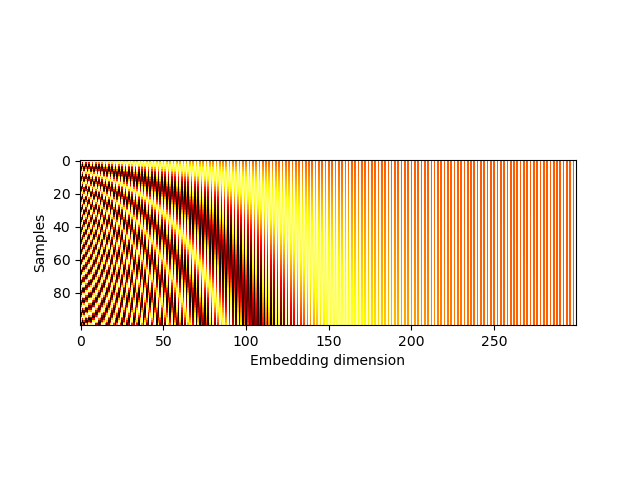
\includegraphics[width=\linewidth]{images/positional_embeddings.png}
        \caption{Heatmap of Positional embeddings for one hundred 300-dimensional samples}
        \label{fig:pos_emb}
    \end{figure}
    
    In this project, an other perspective has been considered : make the positional embedding learnable thanks to the use of learnable embedding layers. 
\end{itemize}

\subsubsection{Attention}

The images being well transformed into sequences and moved into a lower dimensional space, they can now be effectively processed by the network. The network is composed of \textbf{3 blocks} on Figure~\ref{fig:vit_block}, each of them being composed of one \textbf{MultiHeadAttention layer} followed by a \textbf{FeedForward network}, with a skip connection. \\

\begin{figure}[H]
    \centering
    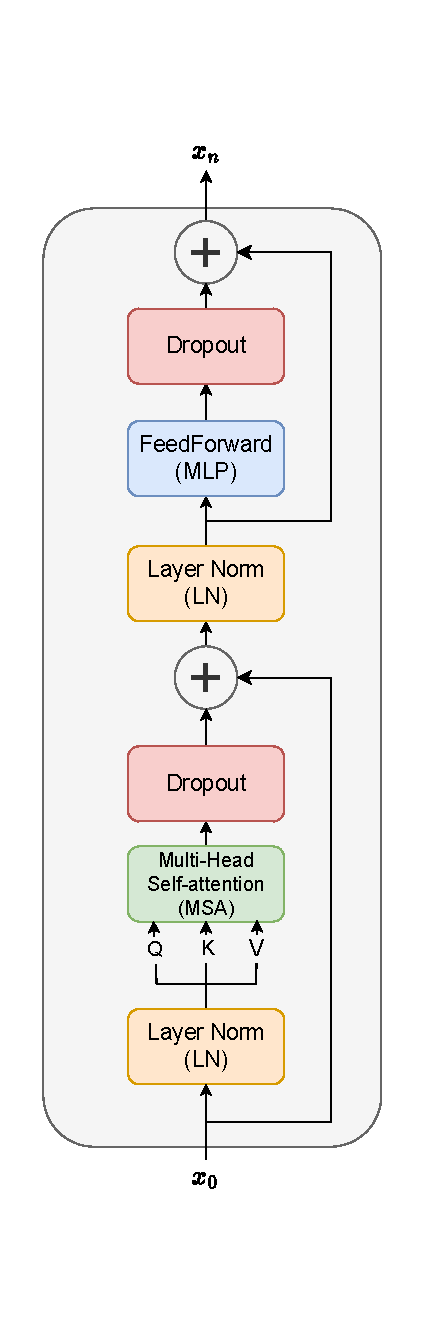
\includegraphics[width=0.5\linewidth]{images/vit_block.pdf}
    \caption{ViT block}
    \label{fig:vit_block}
\end{figure}

The MultiHeadAttention layer defines \textit{n\_heads}, each of them being applied only on a subset of the token embedding. The results of all heads are then merged using concatenation. Each head implements the scaled-dot product attention :

$$
attention(Q,K,V) = softmax \left( \frac{Q K^{T}}{\sqrt{d_k}} \right) V
$$

\begin{figure}[H]
    \begin{flushleft}
        
    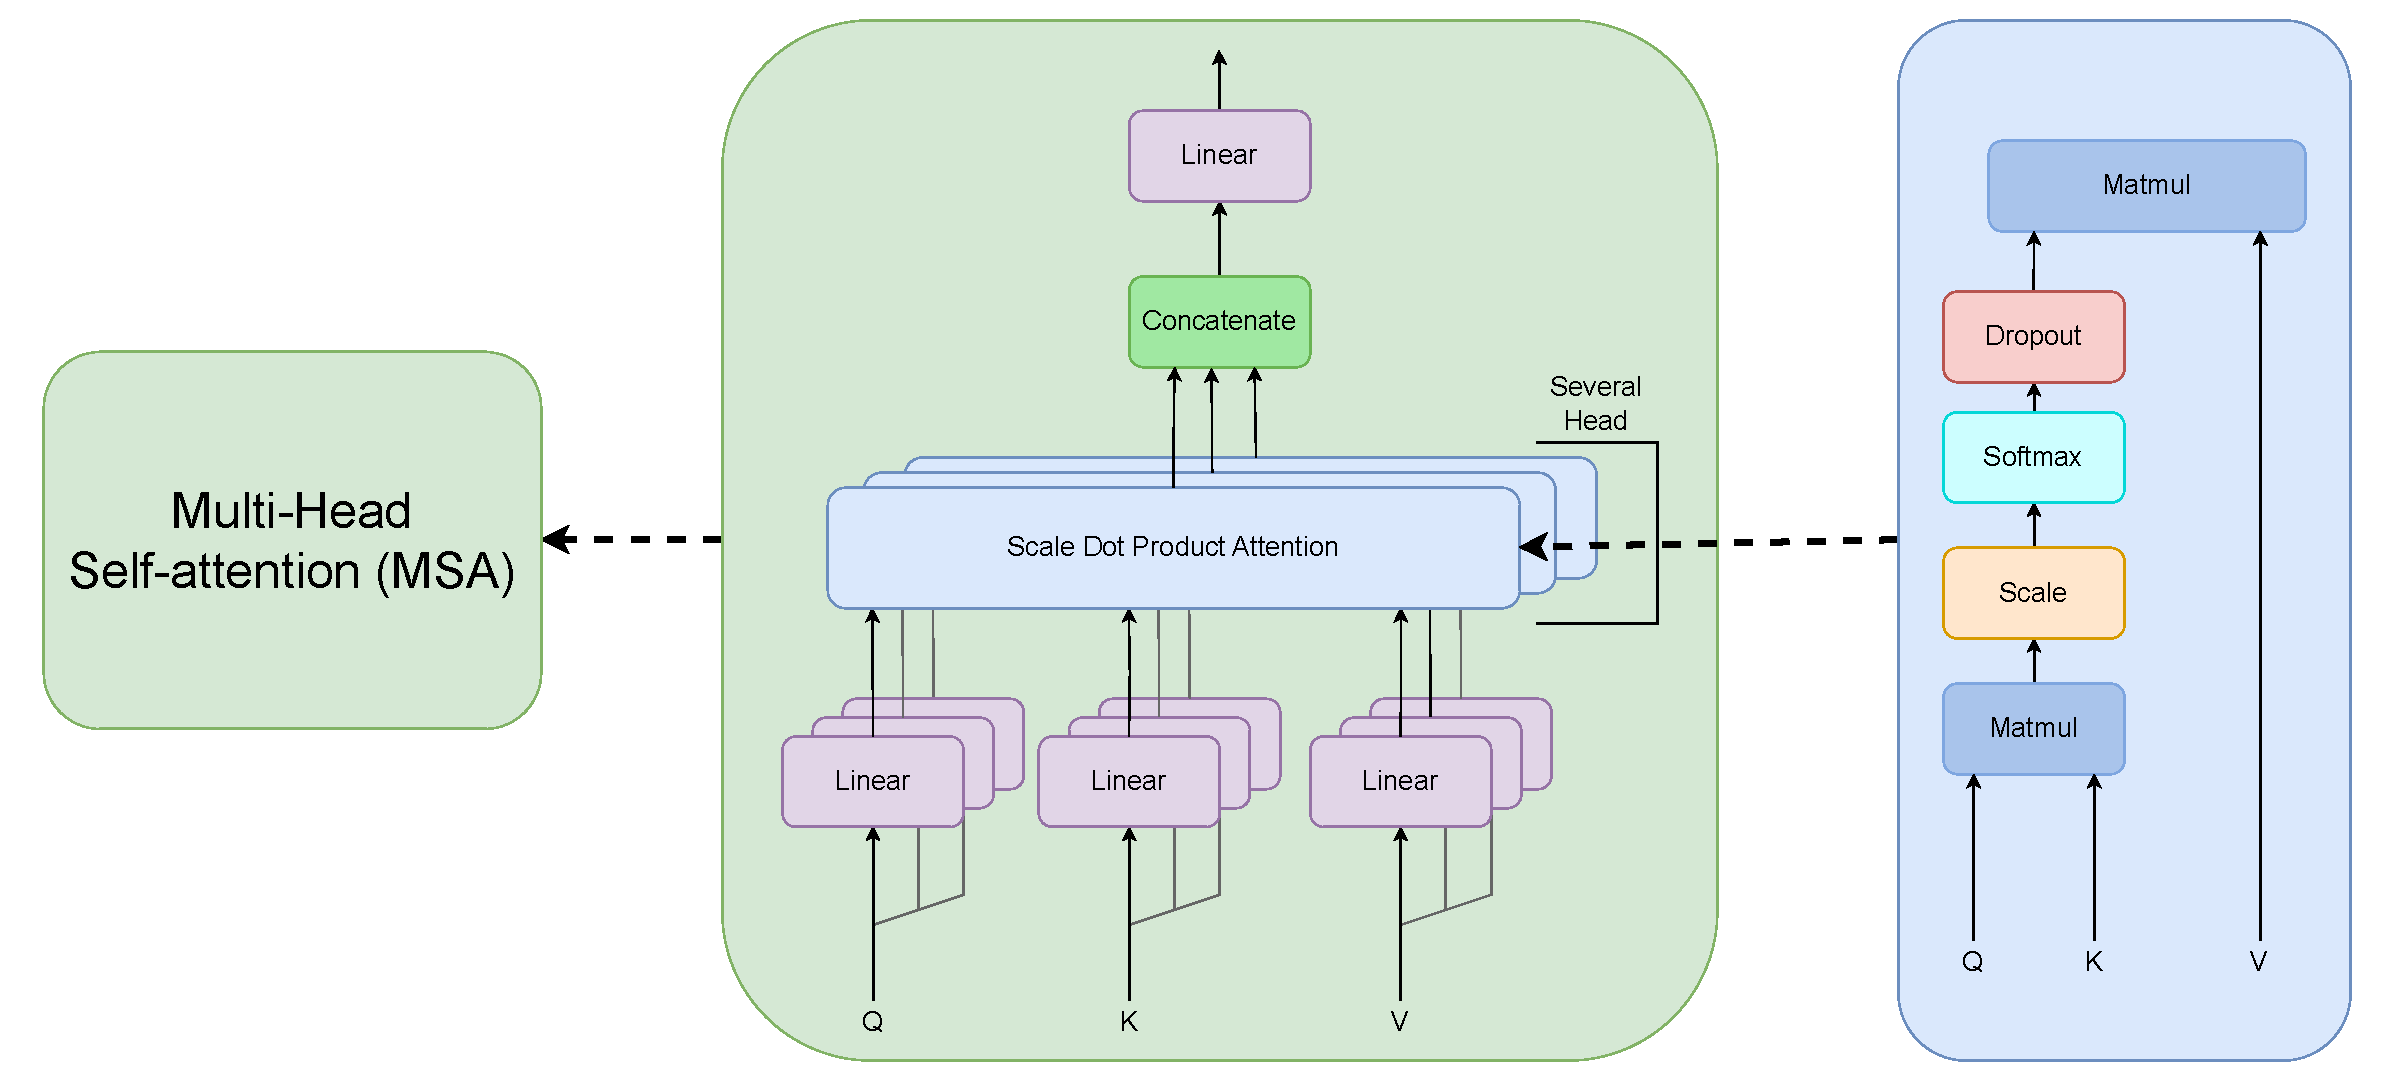
\includegraphics[width=0.9\linewidth]{images/msa_block (1).pdf}
    \caption{MSA block}
    \label{fig:enter-label}
    \end{flushleft}
\end{figure}

This attention mechanism is then followed by a dropout layer. \\

The FeedForward network increases the token dimensions by 4 with a linear layer and then sends the output through an activation function. GeLu is used as activation function here because it is the one used in \cite{vit}, and is known for delivering great results in visual transformer applications. The dimensions are then reduced back by a factor 4. \\

\begin{figure}[H]
    \centering
    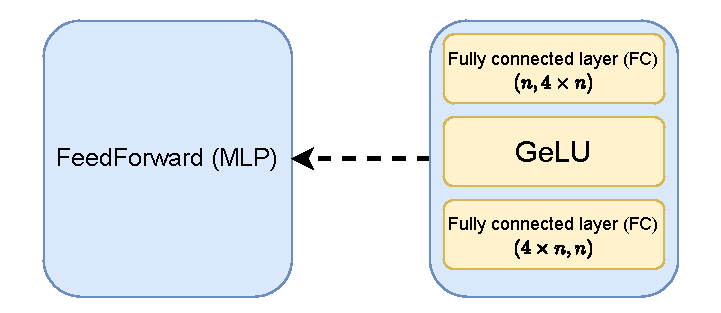
\includegraphics[width=0.75\linewidth]{images/ff_block.pdf}
    \caption{FeedForward block}
    \label{fig:ff_block}
\end{figure}

After the sequence has passed through the 3 blocks, the classification tokens are extracted and fed into a linear layer followed by a softmax layer. This final vector is then used to make predictions.

\subsection{Additional Features}

Additionally, some features are common to all previously explained architectures : 

\begin{itemize}
    \item[$\bullet$] \textbf{Data Augmentation:} The lack of data is a significant limitation for deep learning models. Collecting more data can be expensive and time-consuming, while synthesizing data may not accurately represent true distributions. Image augmentation offers a simple and efficient solution by applying basic transformations to existing data to enhance model performance, by both increasing the size of the dataset and making the model less data-dependent. 

    \item [$\bullet$] \textbf{Optimizer:} The choice of the optimizer is crucial since it defines the algorithm that will update the different parameters of the model. The optimizer that has been chosen for these experiments is \textit{Adam}, very standard for image classification. Adam combines the adpaptative leraning rate of RMSProp and the "inertia" of SGD with momentum, and was found in lots of image classification applications. 

    \item [$\bullet$] \textbf{Stop Criterion:} The stopping criterion for the training phase was defined as a fixed number of iterations. Due to the limited computing resources available, the maximum number of iterations was always set to a very high value such that the training phase was typically stopped by the timeout limit imposed by the GPU providers.

    \item[$\bullet$] \textbf{Weight Initialization:} In convex problems, convergence is guaranteed with a good learning rate regardless of initial parameter values. In non-convex problems, initialization is crucial. ConvNet networks, ResNet, and DenseNet are examples of non-convex problems. Effective initialization should break symmetry and set appropriate weight scales. He initialization, suitable for ReLU activations, initializes weights with variance $\frac{2}{q_l-1}$ to account for non-zero means in activation layers.

    \item[$\bullet$] \textbf{Normalization:} Previous weight initialization strategies rely on maintaining activation variance across layers, assuming constant input feature variances. This assumption is not generally satisfied but can be enforced by standardizing input data feature-wise. Batch normalization maintains proper statistics of activations and derivatives during training, normalizing activations during the forward pass. This ensures stable learning by reducing internal covariate shift.
\end{itemize}


\section{Results}

The dataset used for training and making predictions was the "Places" dataset, which contains 205 classes. Given the large number of classes, high performances were not initially expected. However, upon further reflection, the initial robotics application was reconsidered. For a robot to adapt to its environment, precise classification is not necessary. For instance, a robot does not need to distinguish between a "church" and a "cathedral": it simply needs to recognize that it is in a "monument" environment, prompting it to move slowly and quietly.\\

Consequently, the 205 initial classes were grouped into 17 broader classes to provide an alternative measure of the performances of the same architectures, but trained on slightly different data. This approach also demonstrates how one can adapt publicly available data to suit specific application needs.\\

Despite this adjustment, the performance of the previously described architectures remained below expectations. Therefore, it was decided to train them on a standard dataset (Intel-Images) since the "Places" dataset appeared to be less homogeneous than anticipated. This comparison offers insights into the performance of different architectures across various applications.\\

Both qualitative and quantitative results will be presented in this section, with the four previously detailed models trained on these 3 datasets. 

\subsection{Quantitative Results}

To have a more precise idea of the performances, some metrics have been plotted during the training phase. The three quantities of interest are : the training loss, the testing loss and the accuracy. The loss that was chosen is the \textit{Cross Entropy Loss}, which is standard for classification. It is defined has followed : 

$$
H(p,q) = -\mathbb{E}_p [log(q)]
$$

Where p is the real groundtruth while q is the estimated probability distribution given by the output softmax layer. Accuracy is defined as the proportion of correct predictions on the test set. \\


\subsubsection{InteImages}

These three quantities have been plotted for the different architectures at first on the dataset \textit{IntelImages}, as can be seen on Fig. \ref{fig:intel}. 

\begin{figure}[H]
    \centering
    \begin{subfigure}{0.235 \textwidth}
        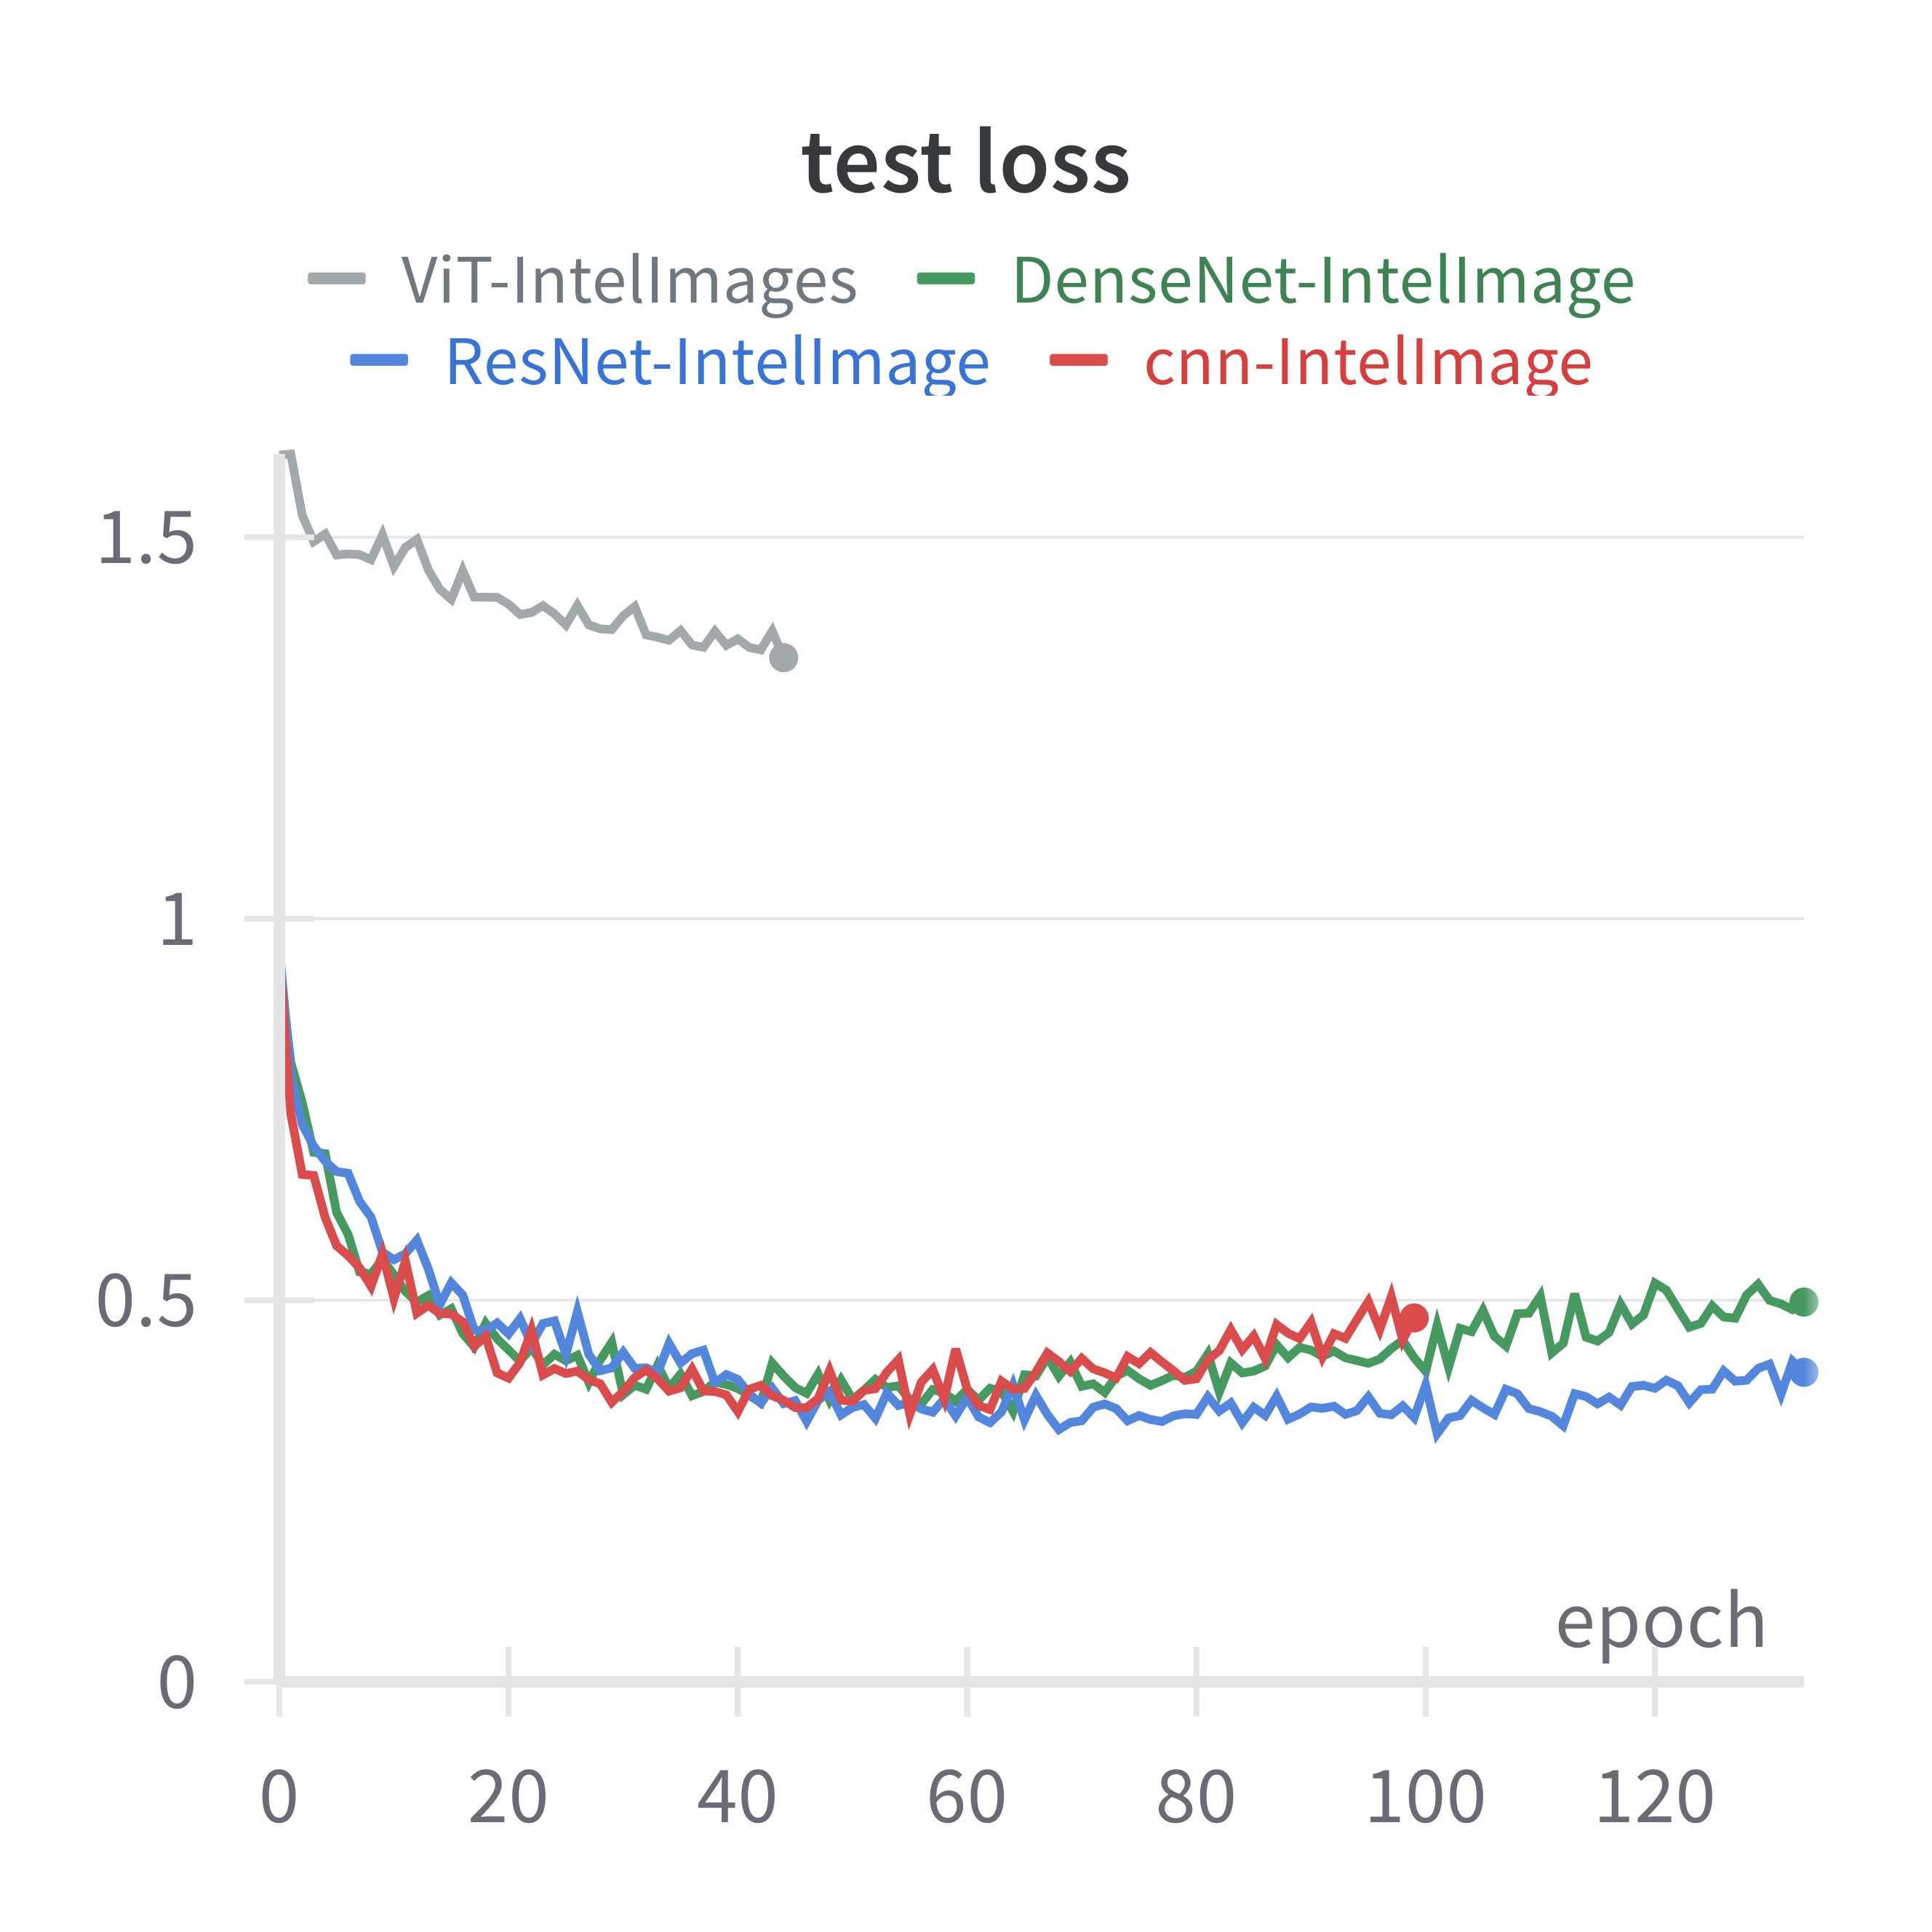
\includegraphics[width = 0.99 \textwidth]{images/IntelImage_test.png}
        \caption{Test Loss}
    \end{subfigure}
    \begin{subfigure}{0.235 \textwidth}
        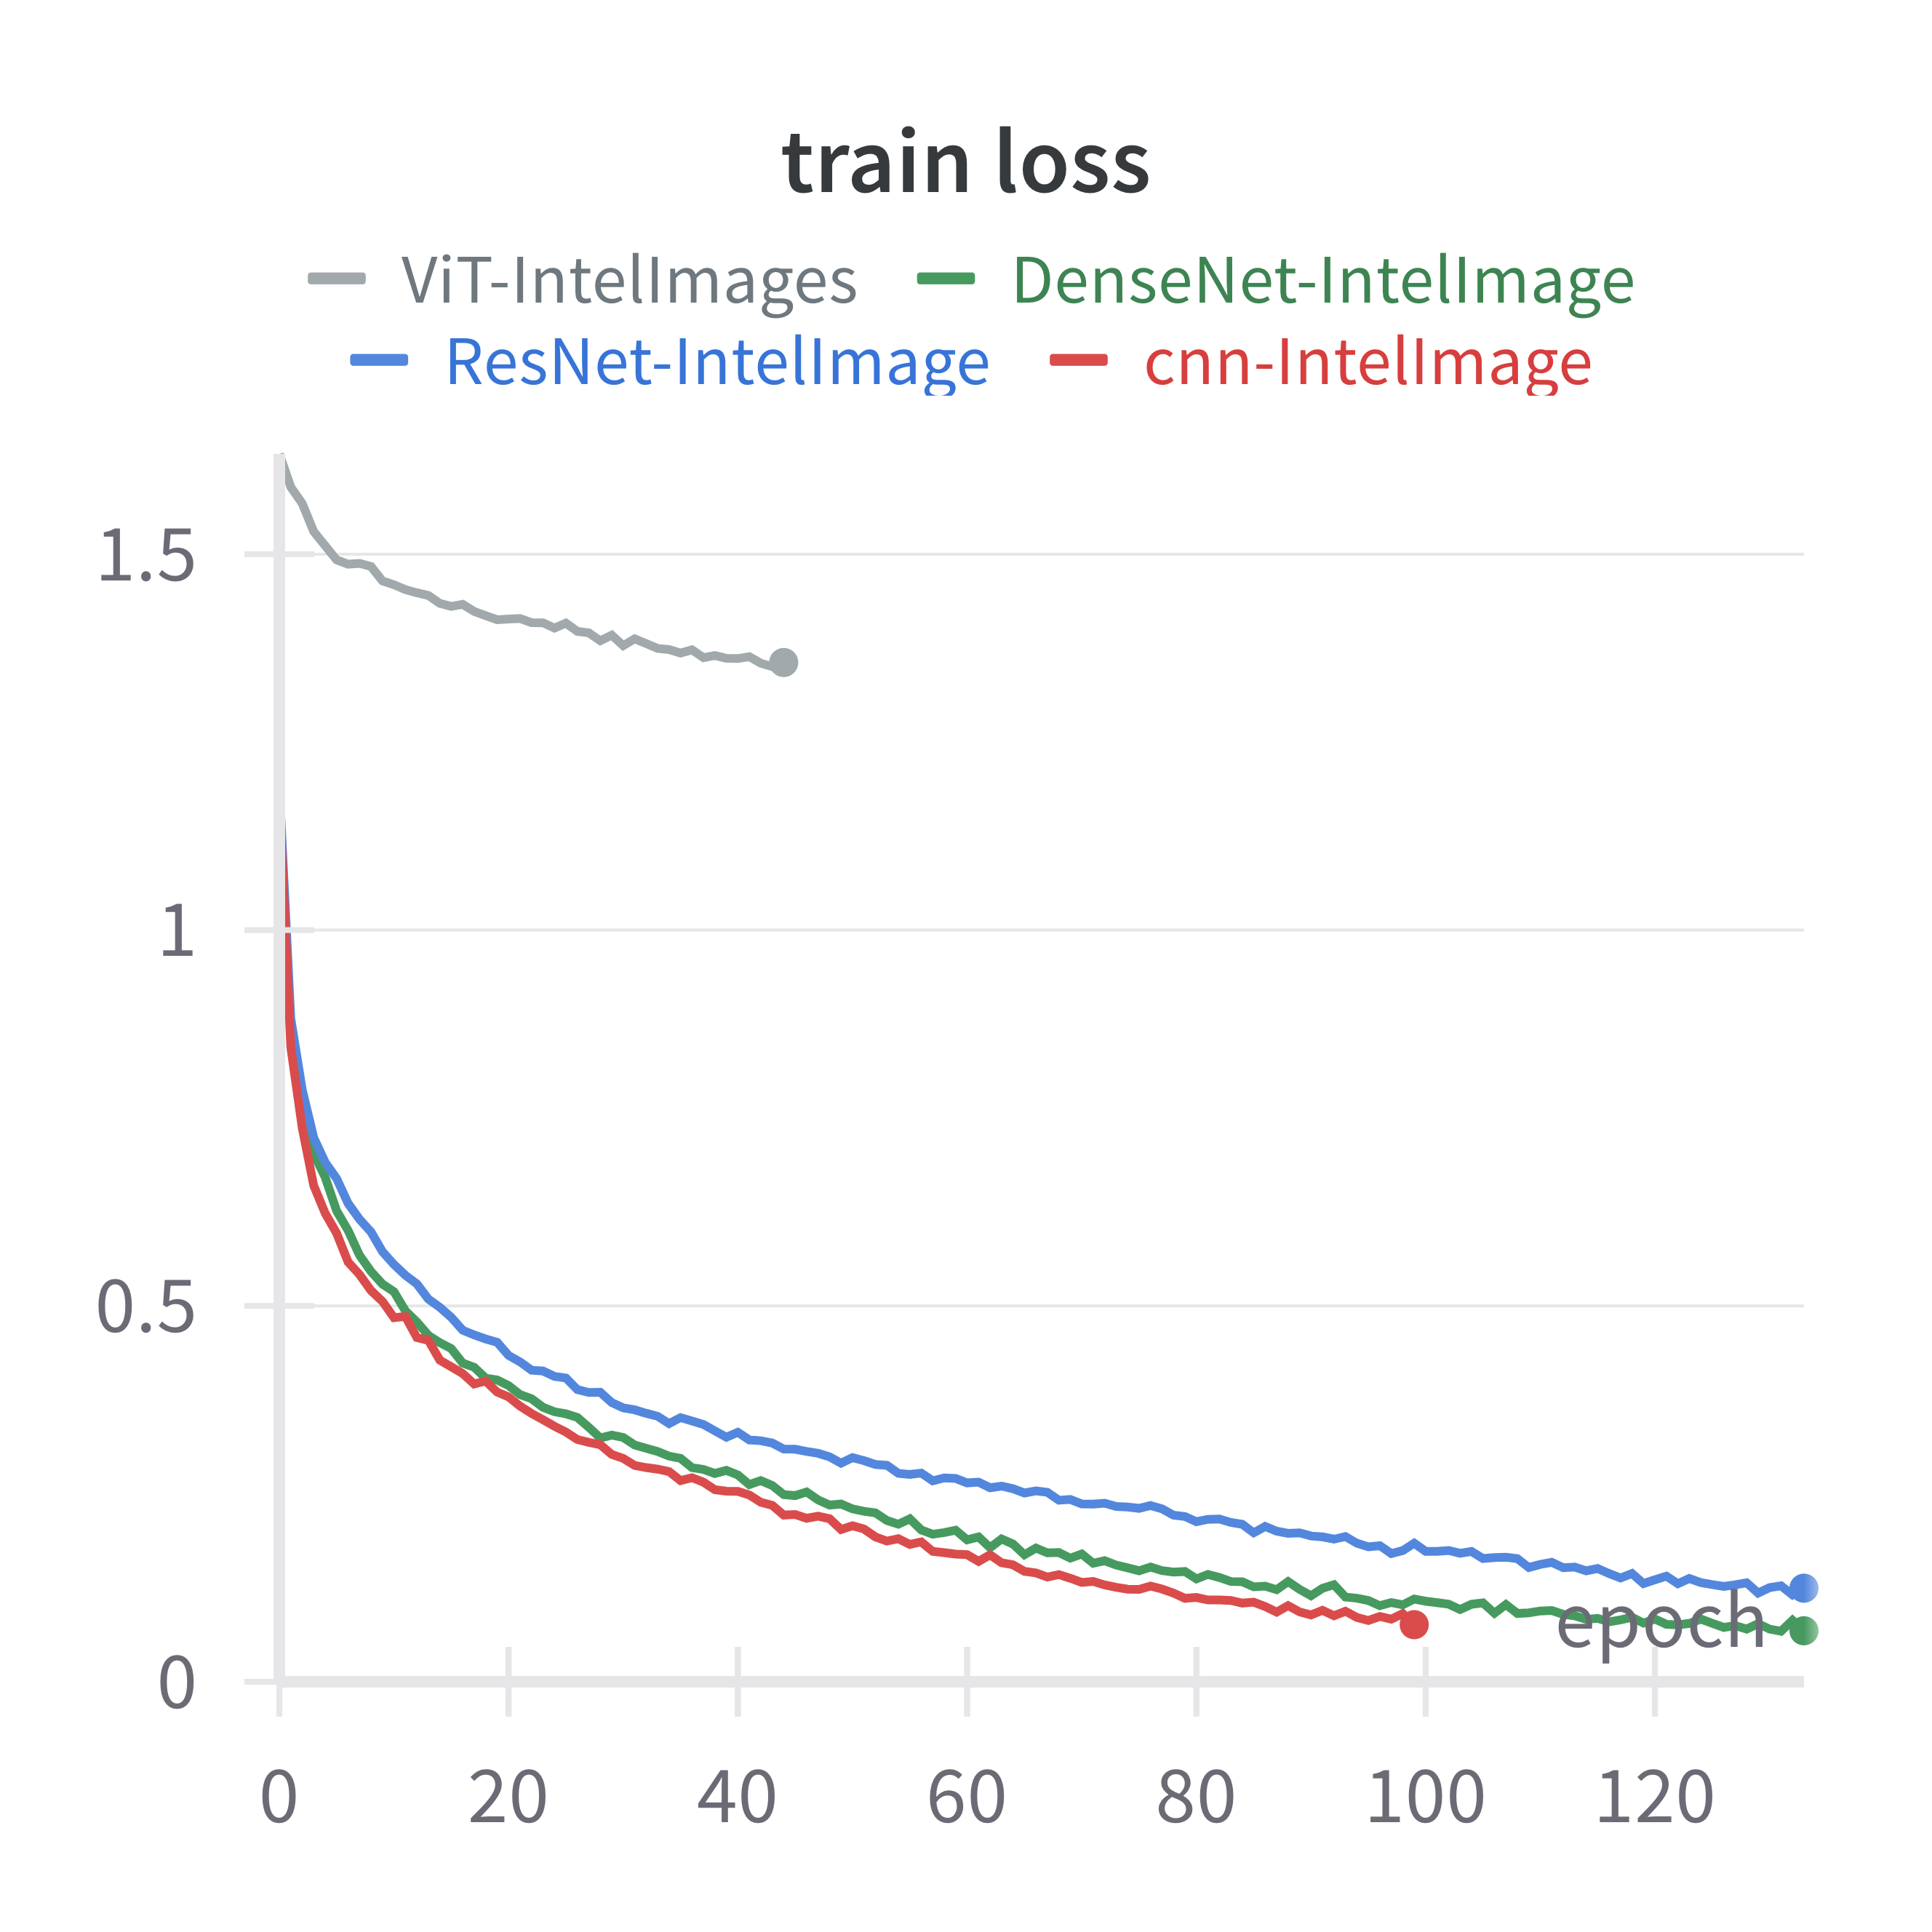
\includegraphics[width = 0.99 \textwidth]{images/IntelImage_train.png}
        \caption{Train Loss}
    \end{subfigure}
    \begin{subfigure}{0.35 \textwidth}
        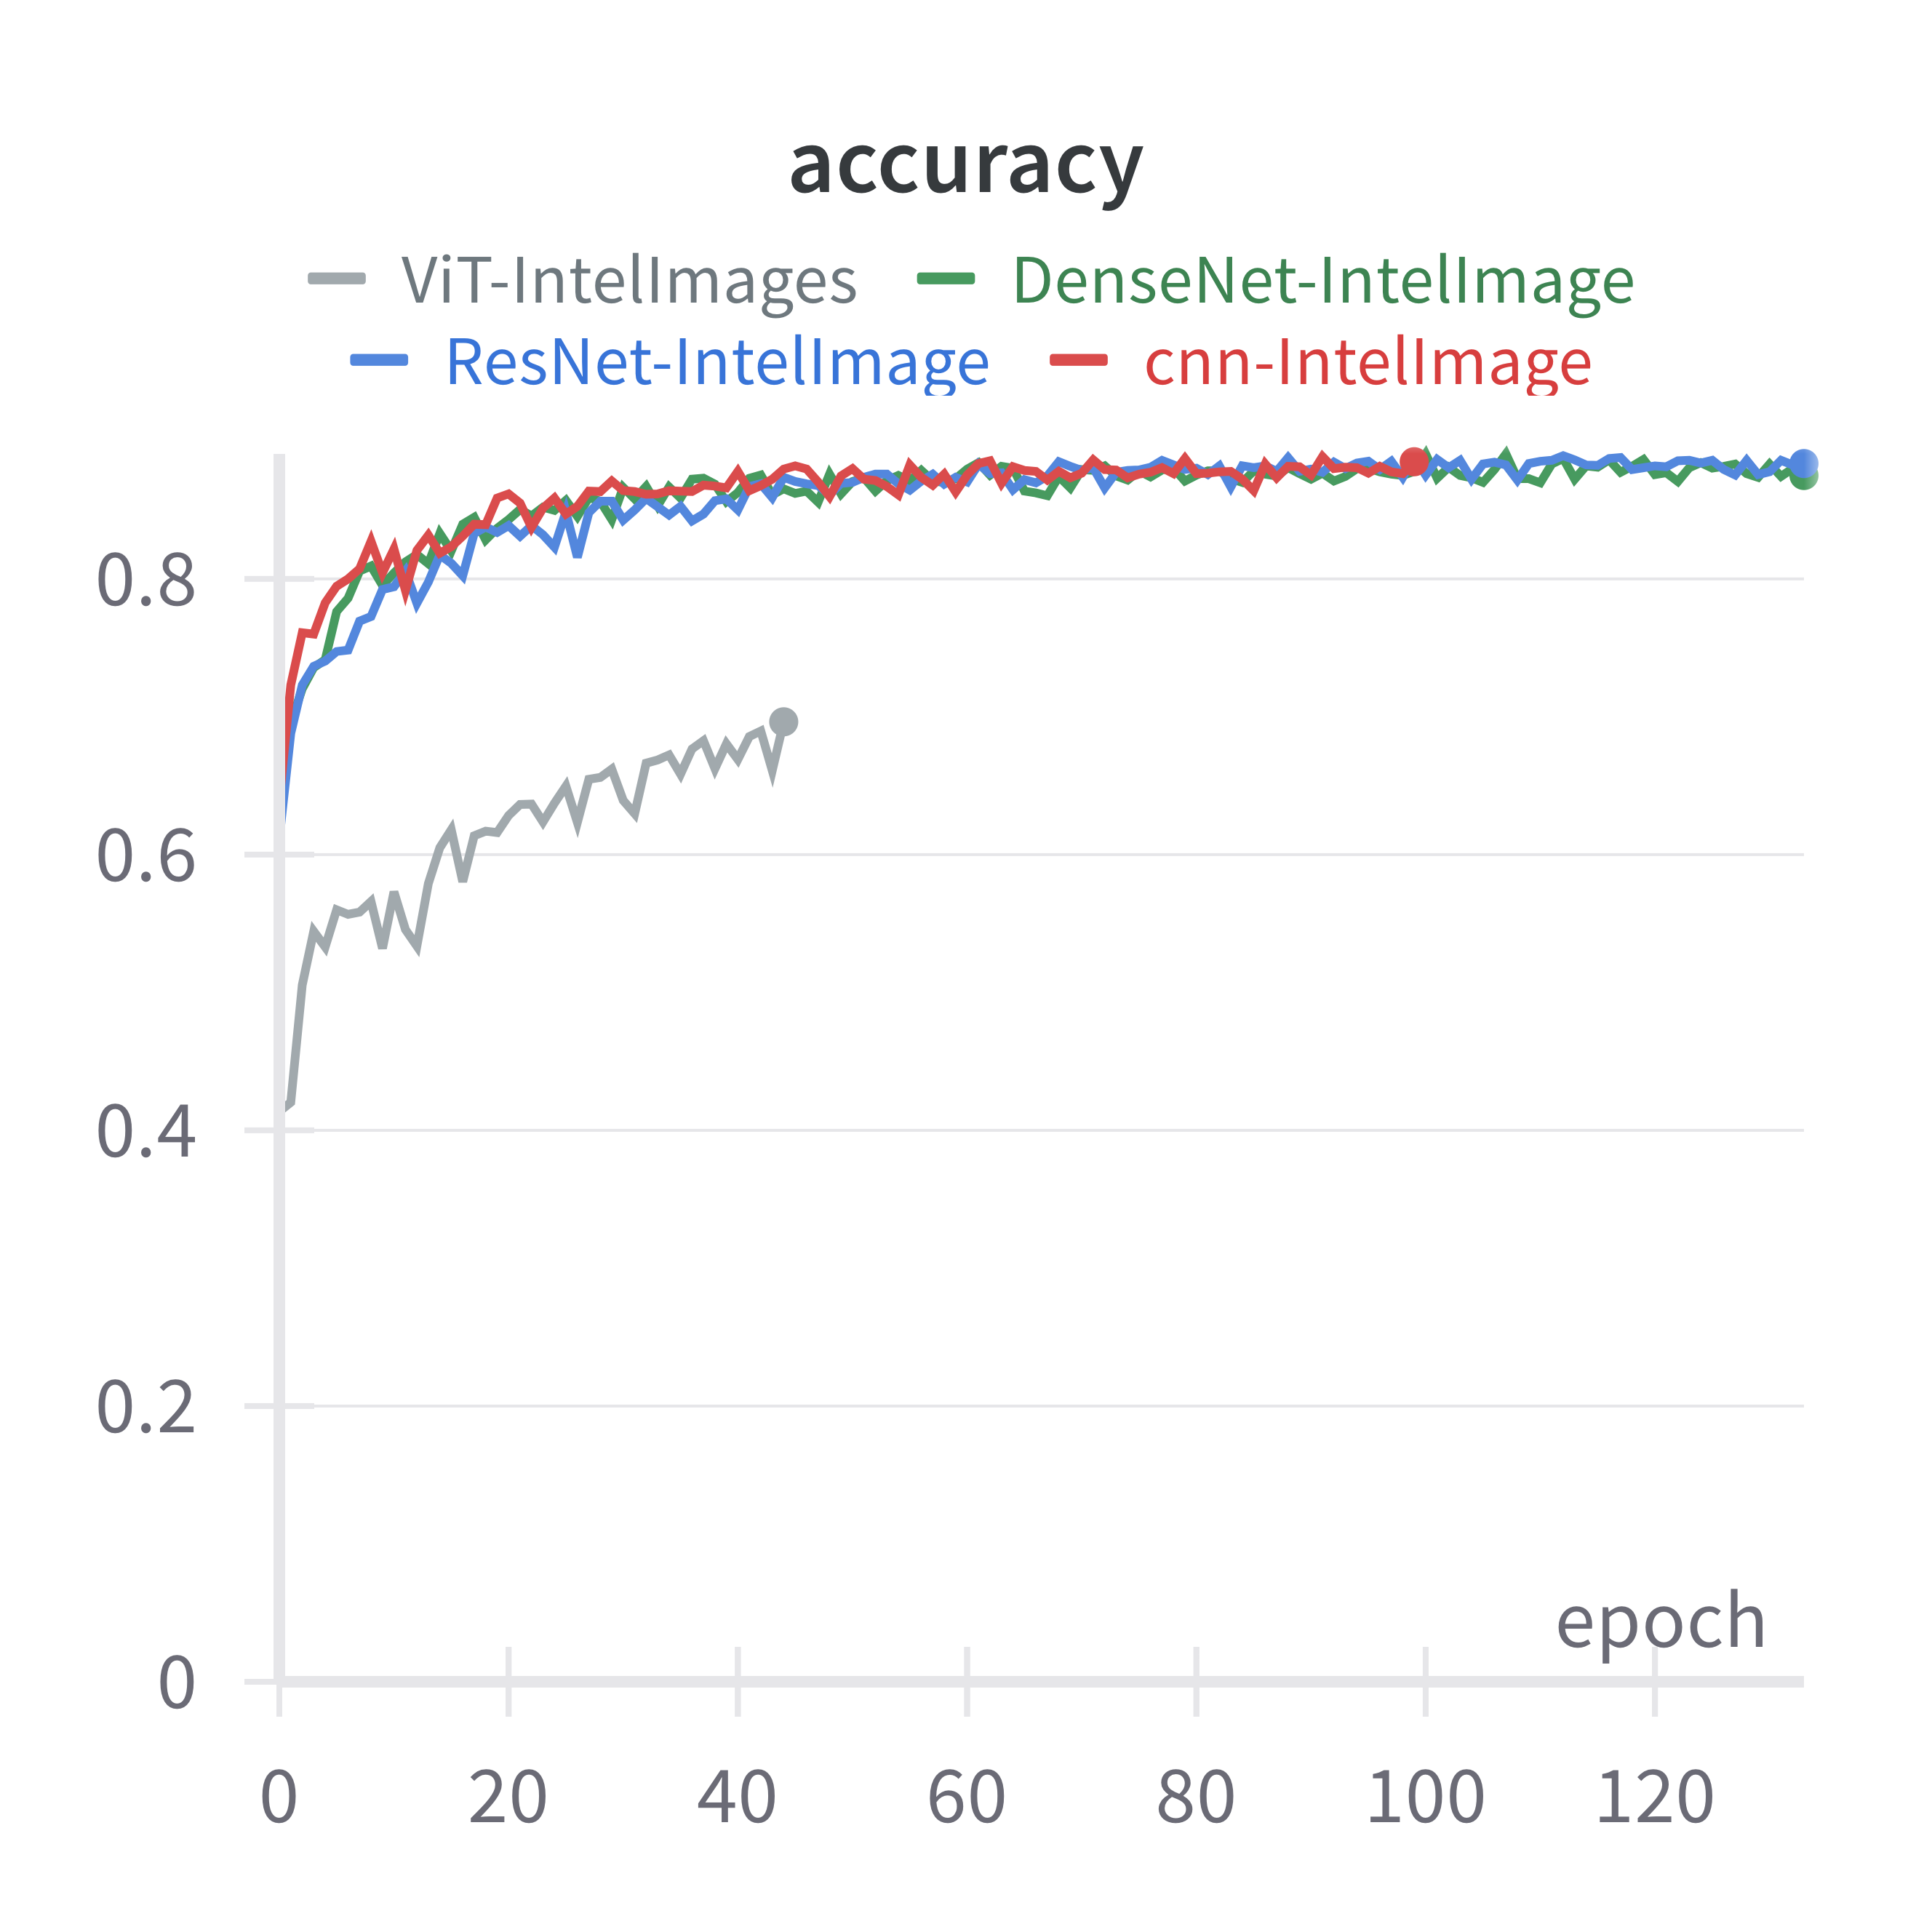
\includegraphics[width = 0.99 \textwidth]{images/IntelImage_accuracy.png}
        \caption{Accuracy}
    \end{subfigure}
    
    \caption{Performances of the different considered architectures on the dataset \textit{IntelImages}}
    \label{fig:intel}
\end{figure}

The performances of the ConvNet, ResNet, and DenseNet are very similar, while the Vision Transformer exhibits significantly lower accuracy and higher losses. However, because the Vision Transformer does not benefit from the inductive biases of convolutional architectures (such as translation invariance and locality), it requires more time to build an accurate representation of the data. Consequently, this model might have shown better performances if it had been trained for a longer number of iterations. Another way to support this is by examining the test losses: all convolutional networks reached their minimum around epoch 50, whereas the Vision Transformer had not yet reached its minimum, indicating that its performance could still be improved.\\

\subsubsection{Convolutional Architectures}

Since the "Places" dataset is much larger than the IntelImages dataset (around 1500 images per class, totaling approximately 300,000 images) and the Vision Transformer architecture is more computationally demanding than convolutional networks, it was not feasible to train them for the same number of epochs. Therefore, the analysis will be divided into two parts to keep the graphs in the same order of magnitude. The performances of the ConvNet, ResNet, and DenseNet on the full "Places" dataset are shown in Fig. \ref{fig:205_convnets}. As observed, ResNet and DenseNet demonstrate better performances compared to the standard ConvNet architecture, attributable to their increased depth enabled by the introduction of skip connections. Among these, DenseNet performs the best, although it appears that ResNet could have achieved better performance if it had been trained for a longer duration. Overall, the best achievable performance is around 40\%.\\

\begin{figure}[H]
    \centering
    \begin{subfigure}{0.235 \textwidth}
        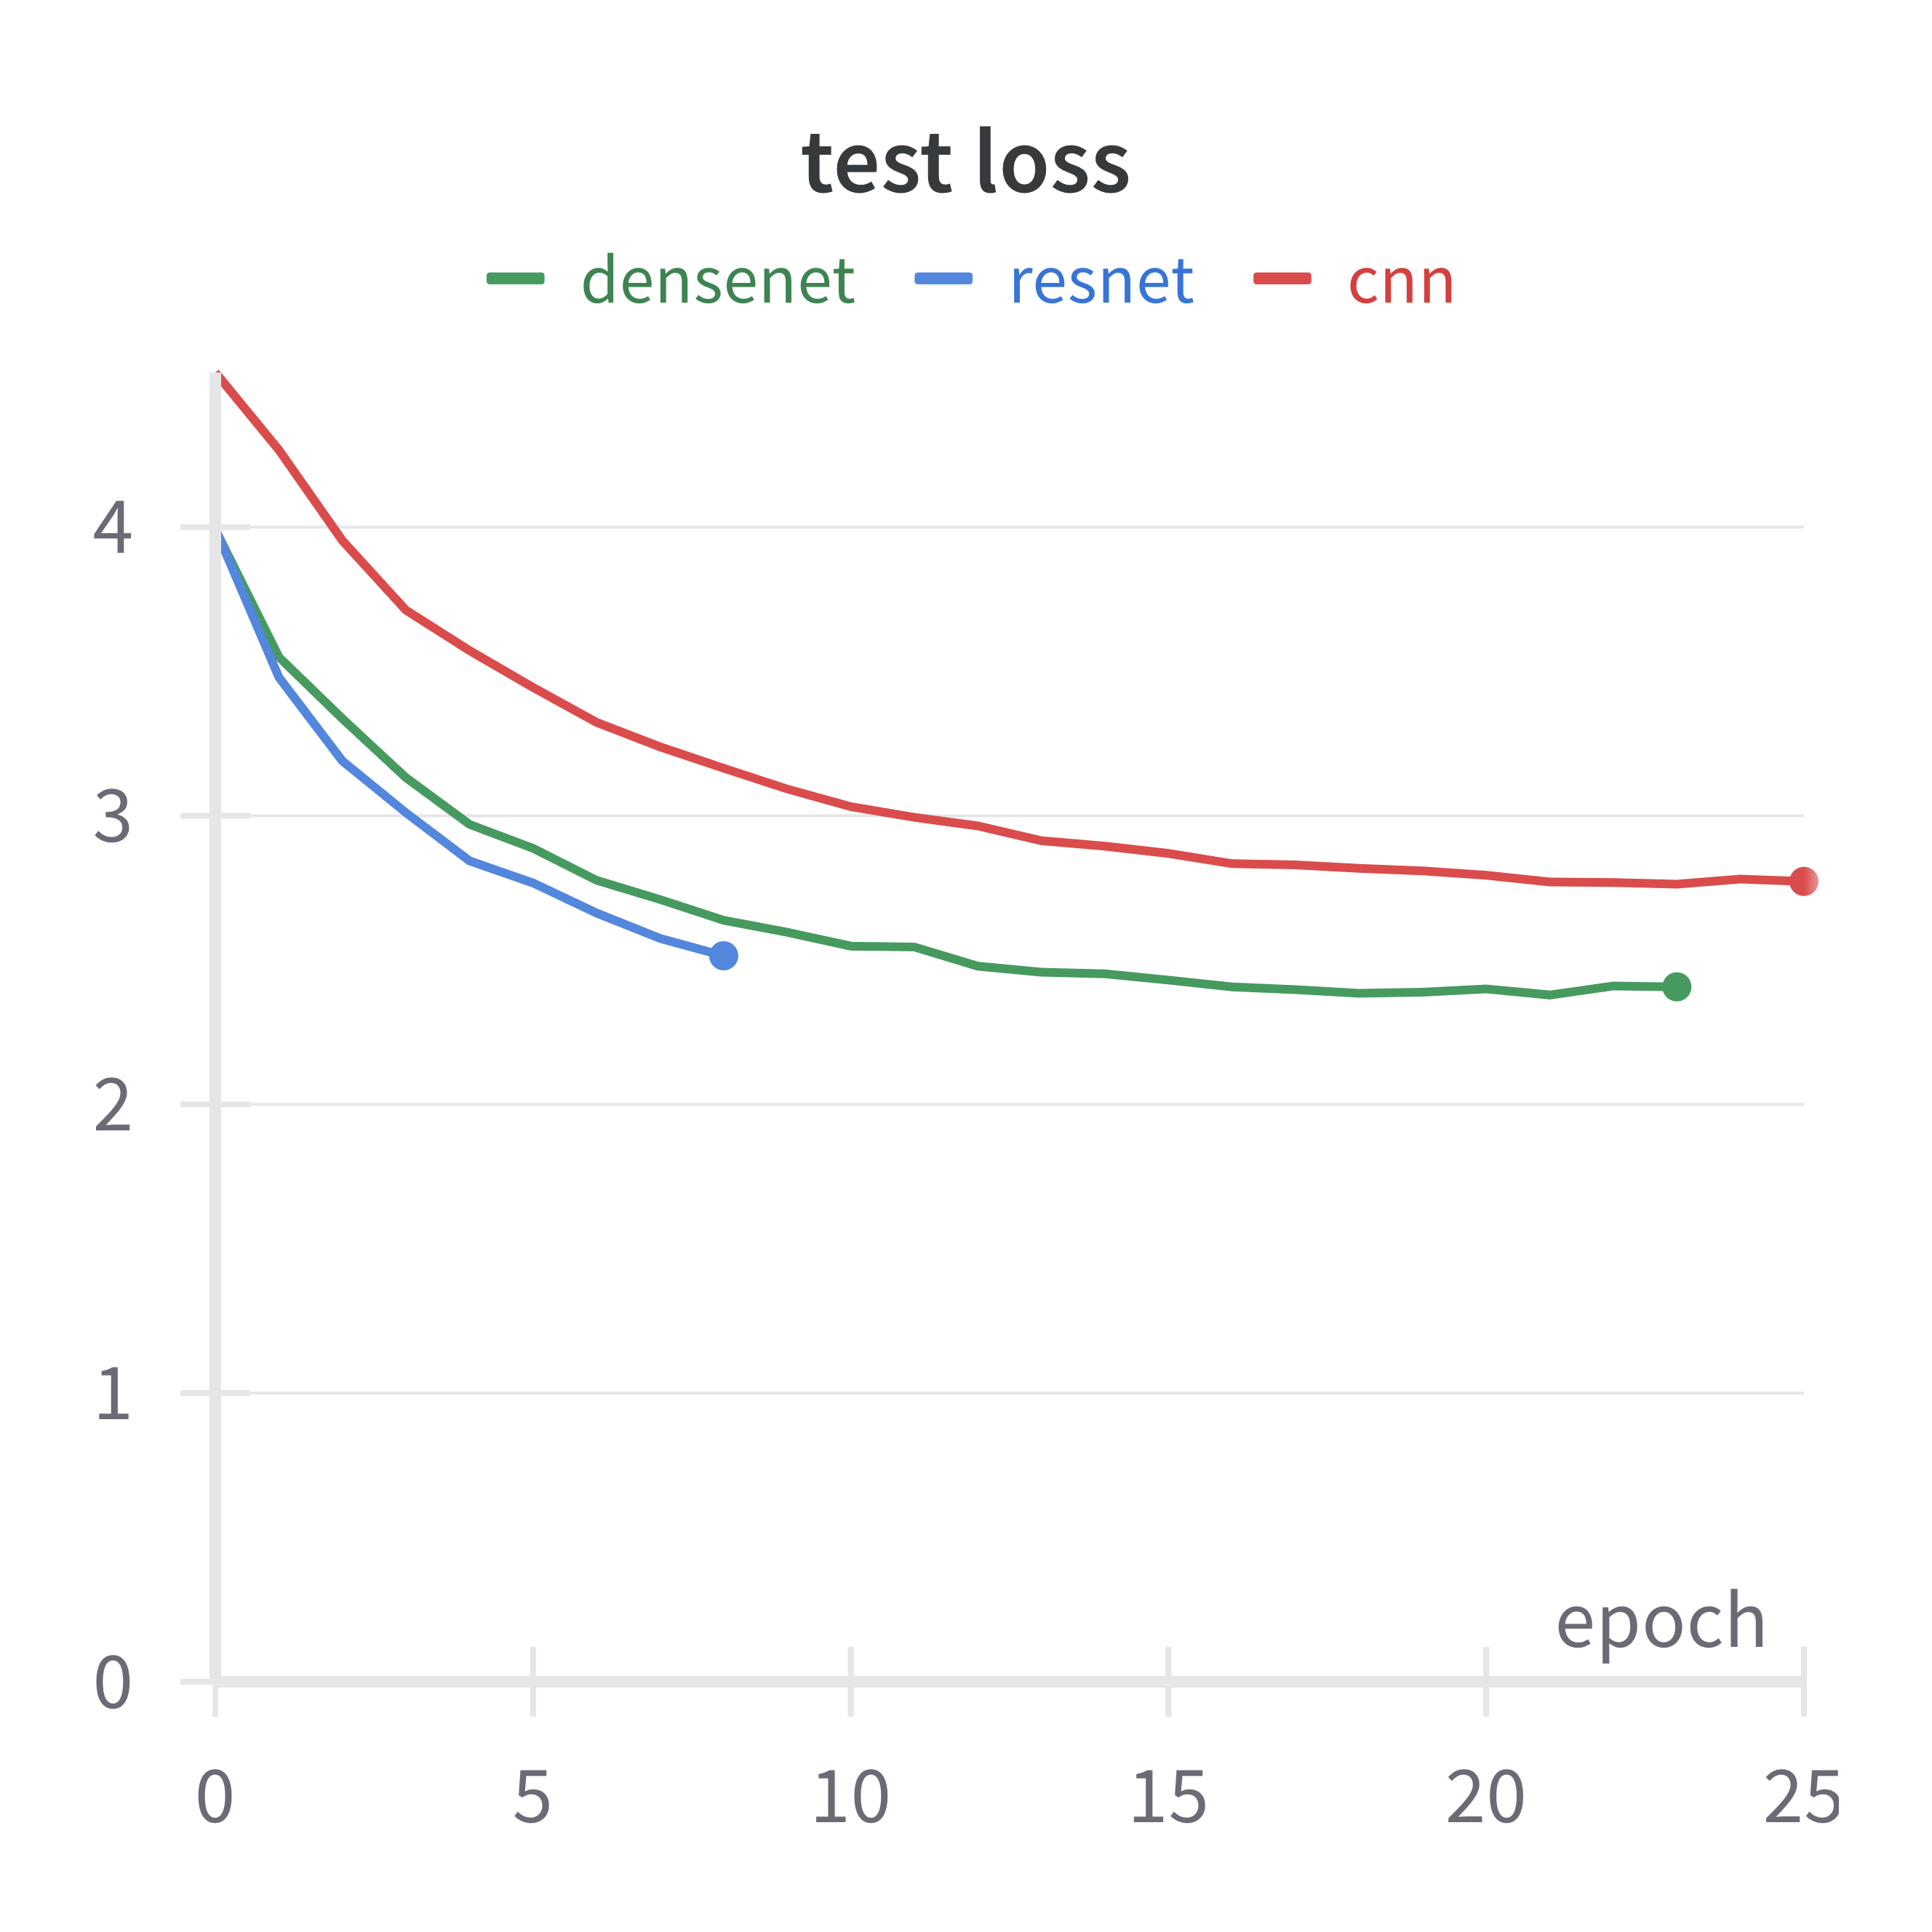
\includegraphics[width = 0.99 \textwidth]{images/205classes_test.png}
        \caption{Test Loss}
    \end{subfigure}
    \begin{subfigure}{0.235 \textwidth}
        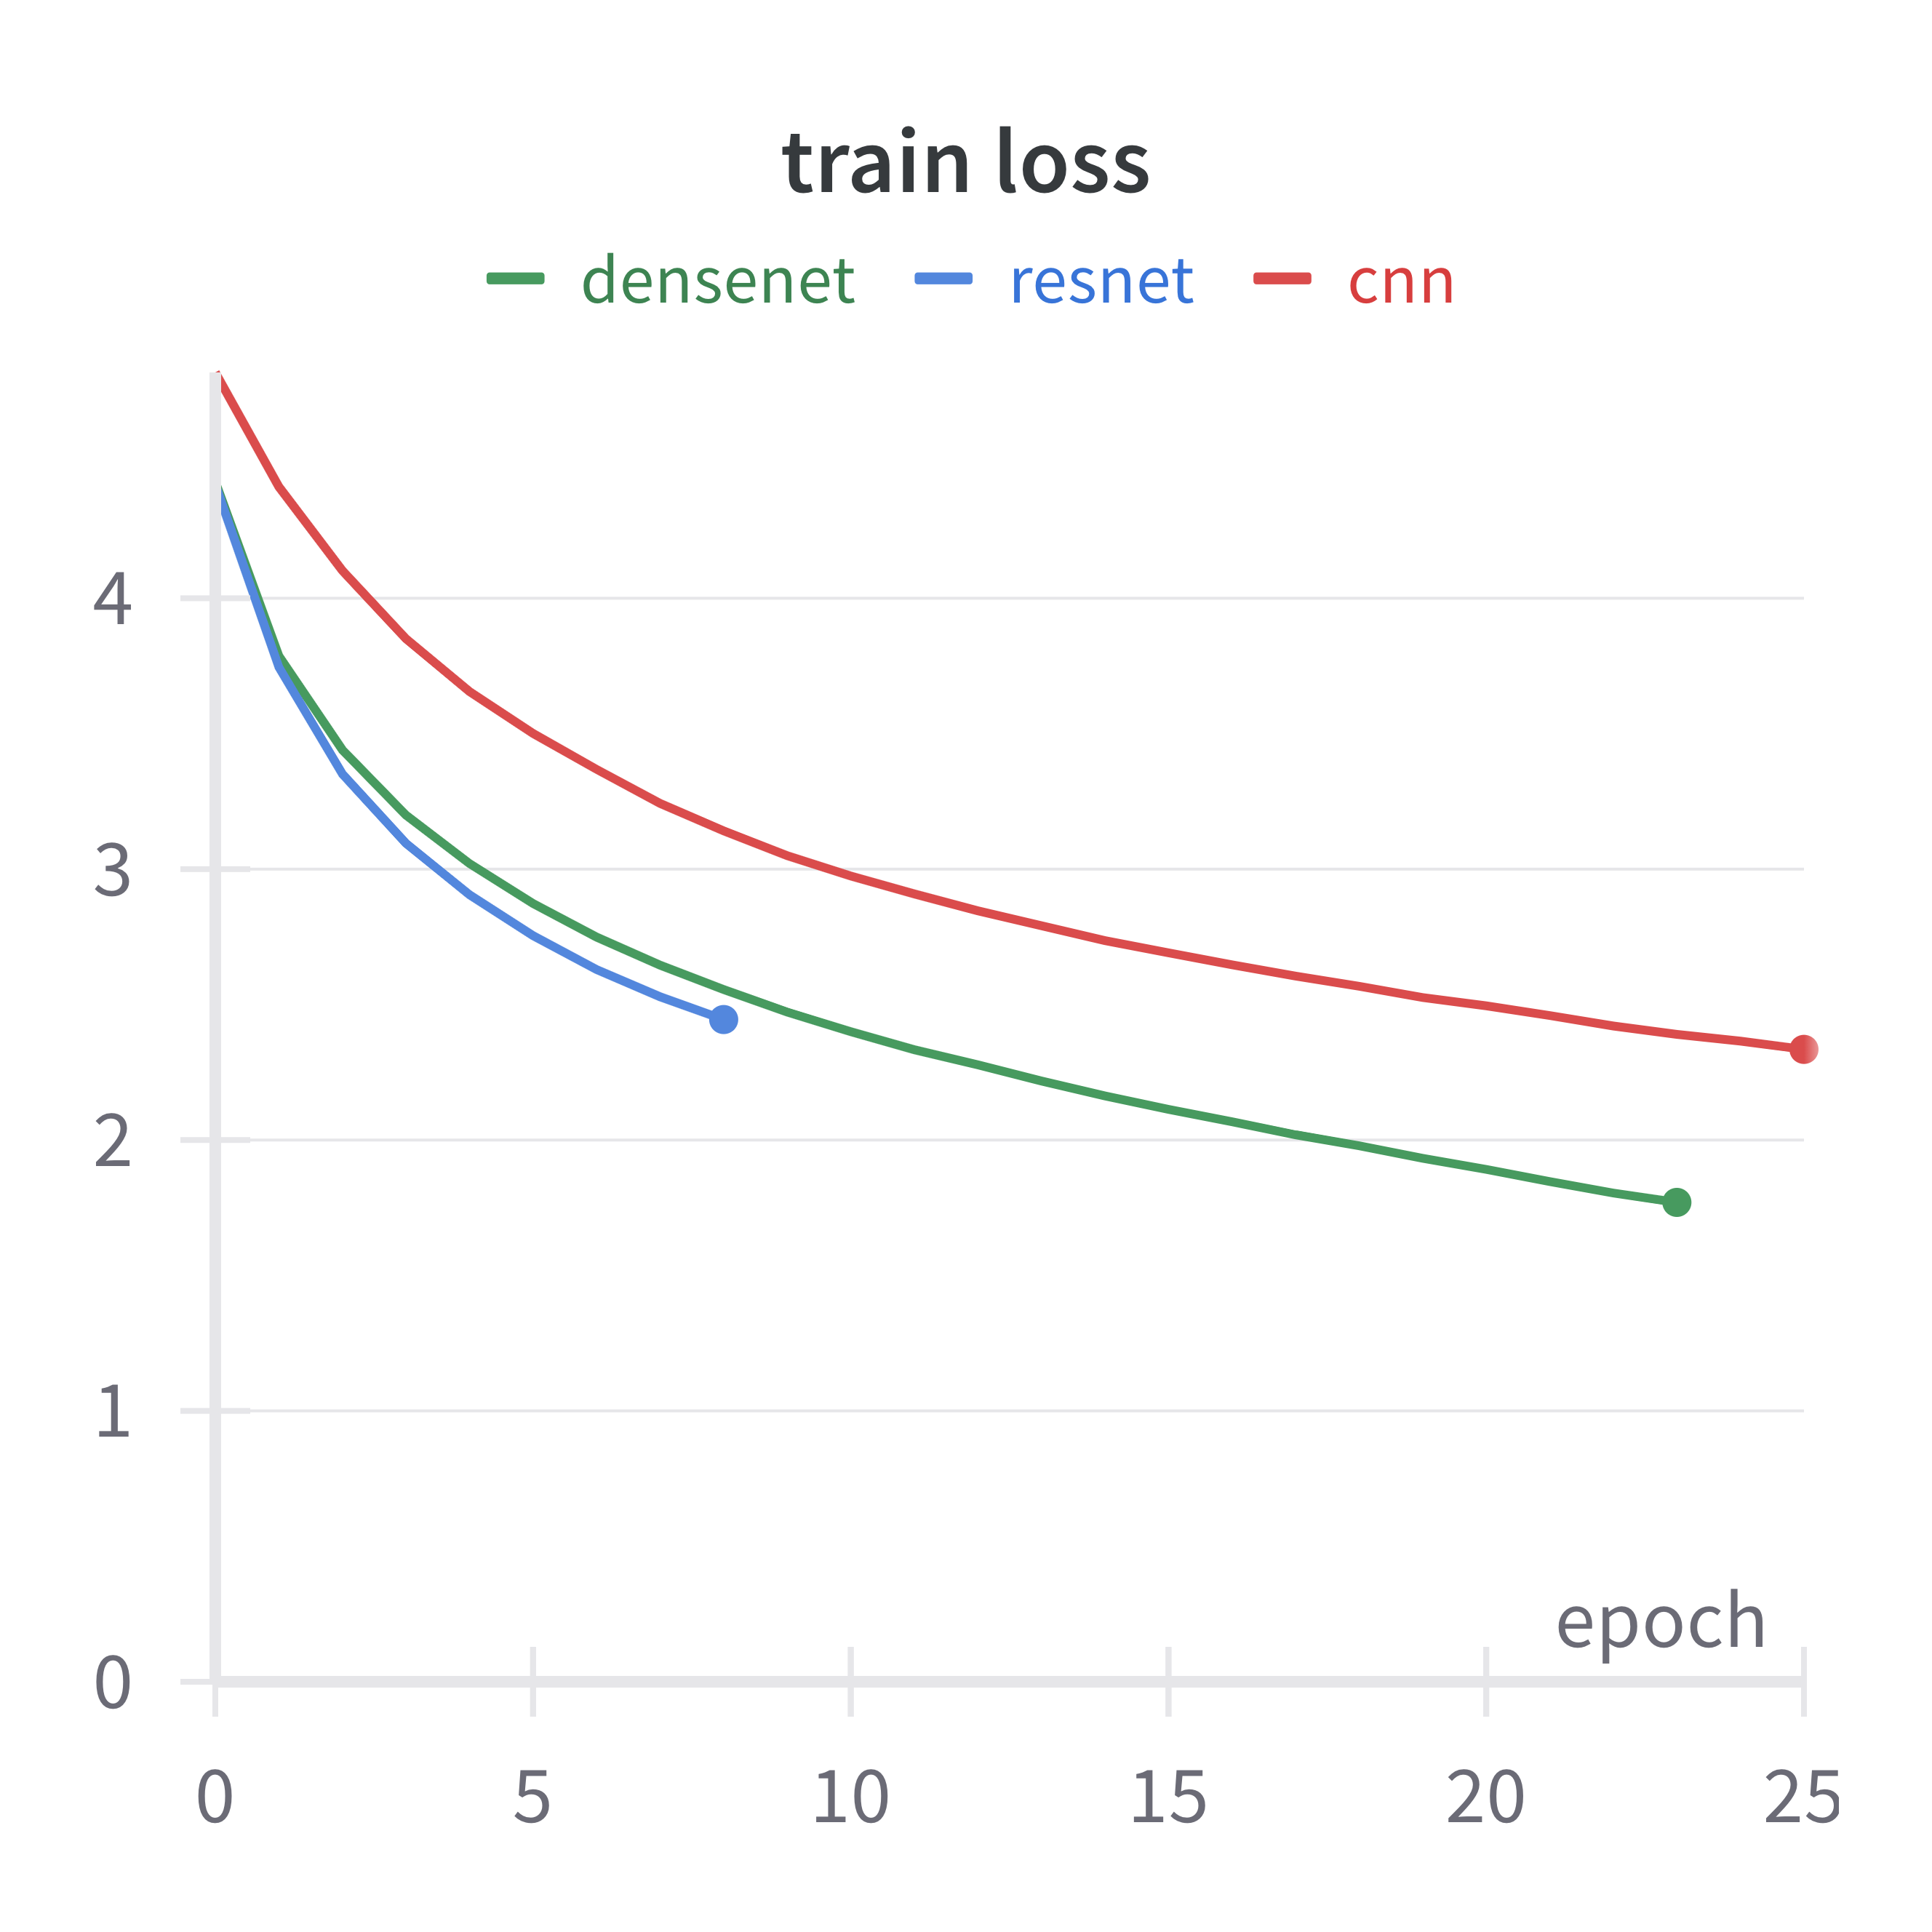
\includegraphics[width = 0.99 \textwidth]{images/205classes_train.png}
        \caption{Train Loss}
    \end{subfigure}
    \begin{subfigure}{0.35 \textwidth}
        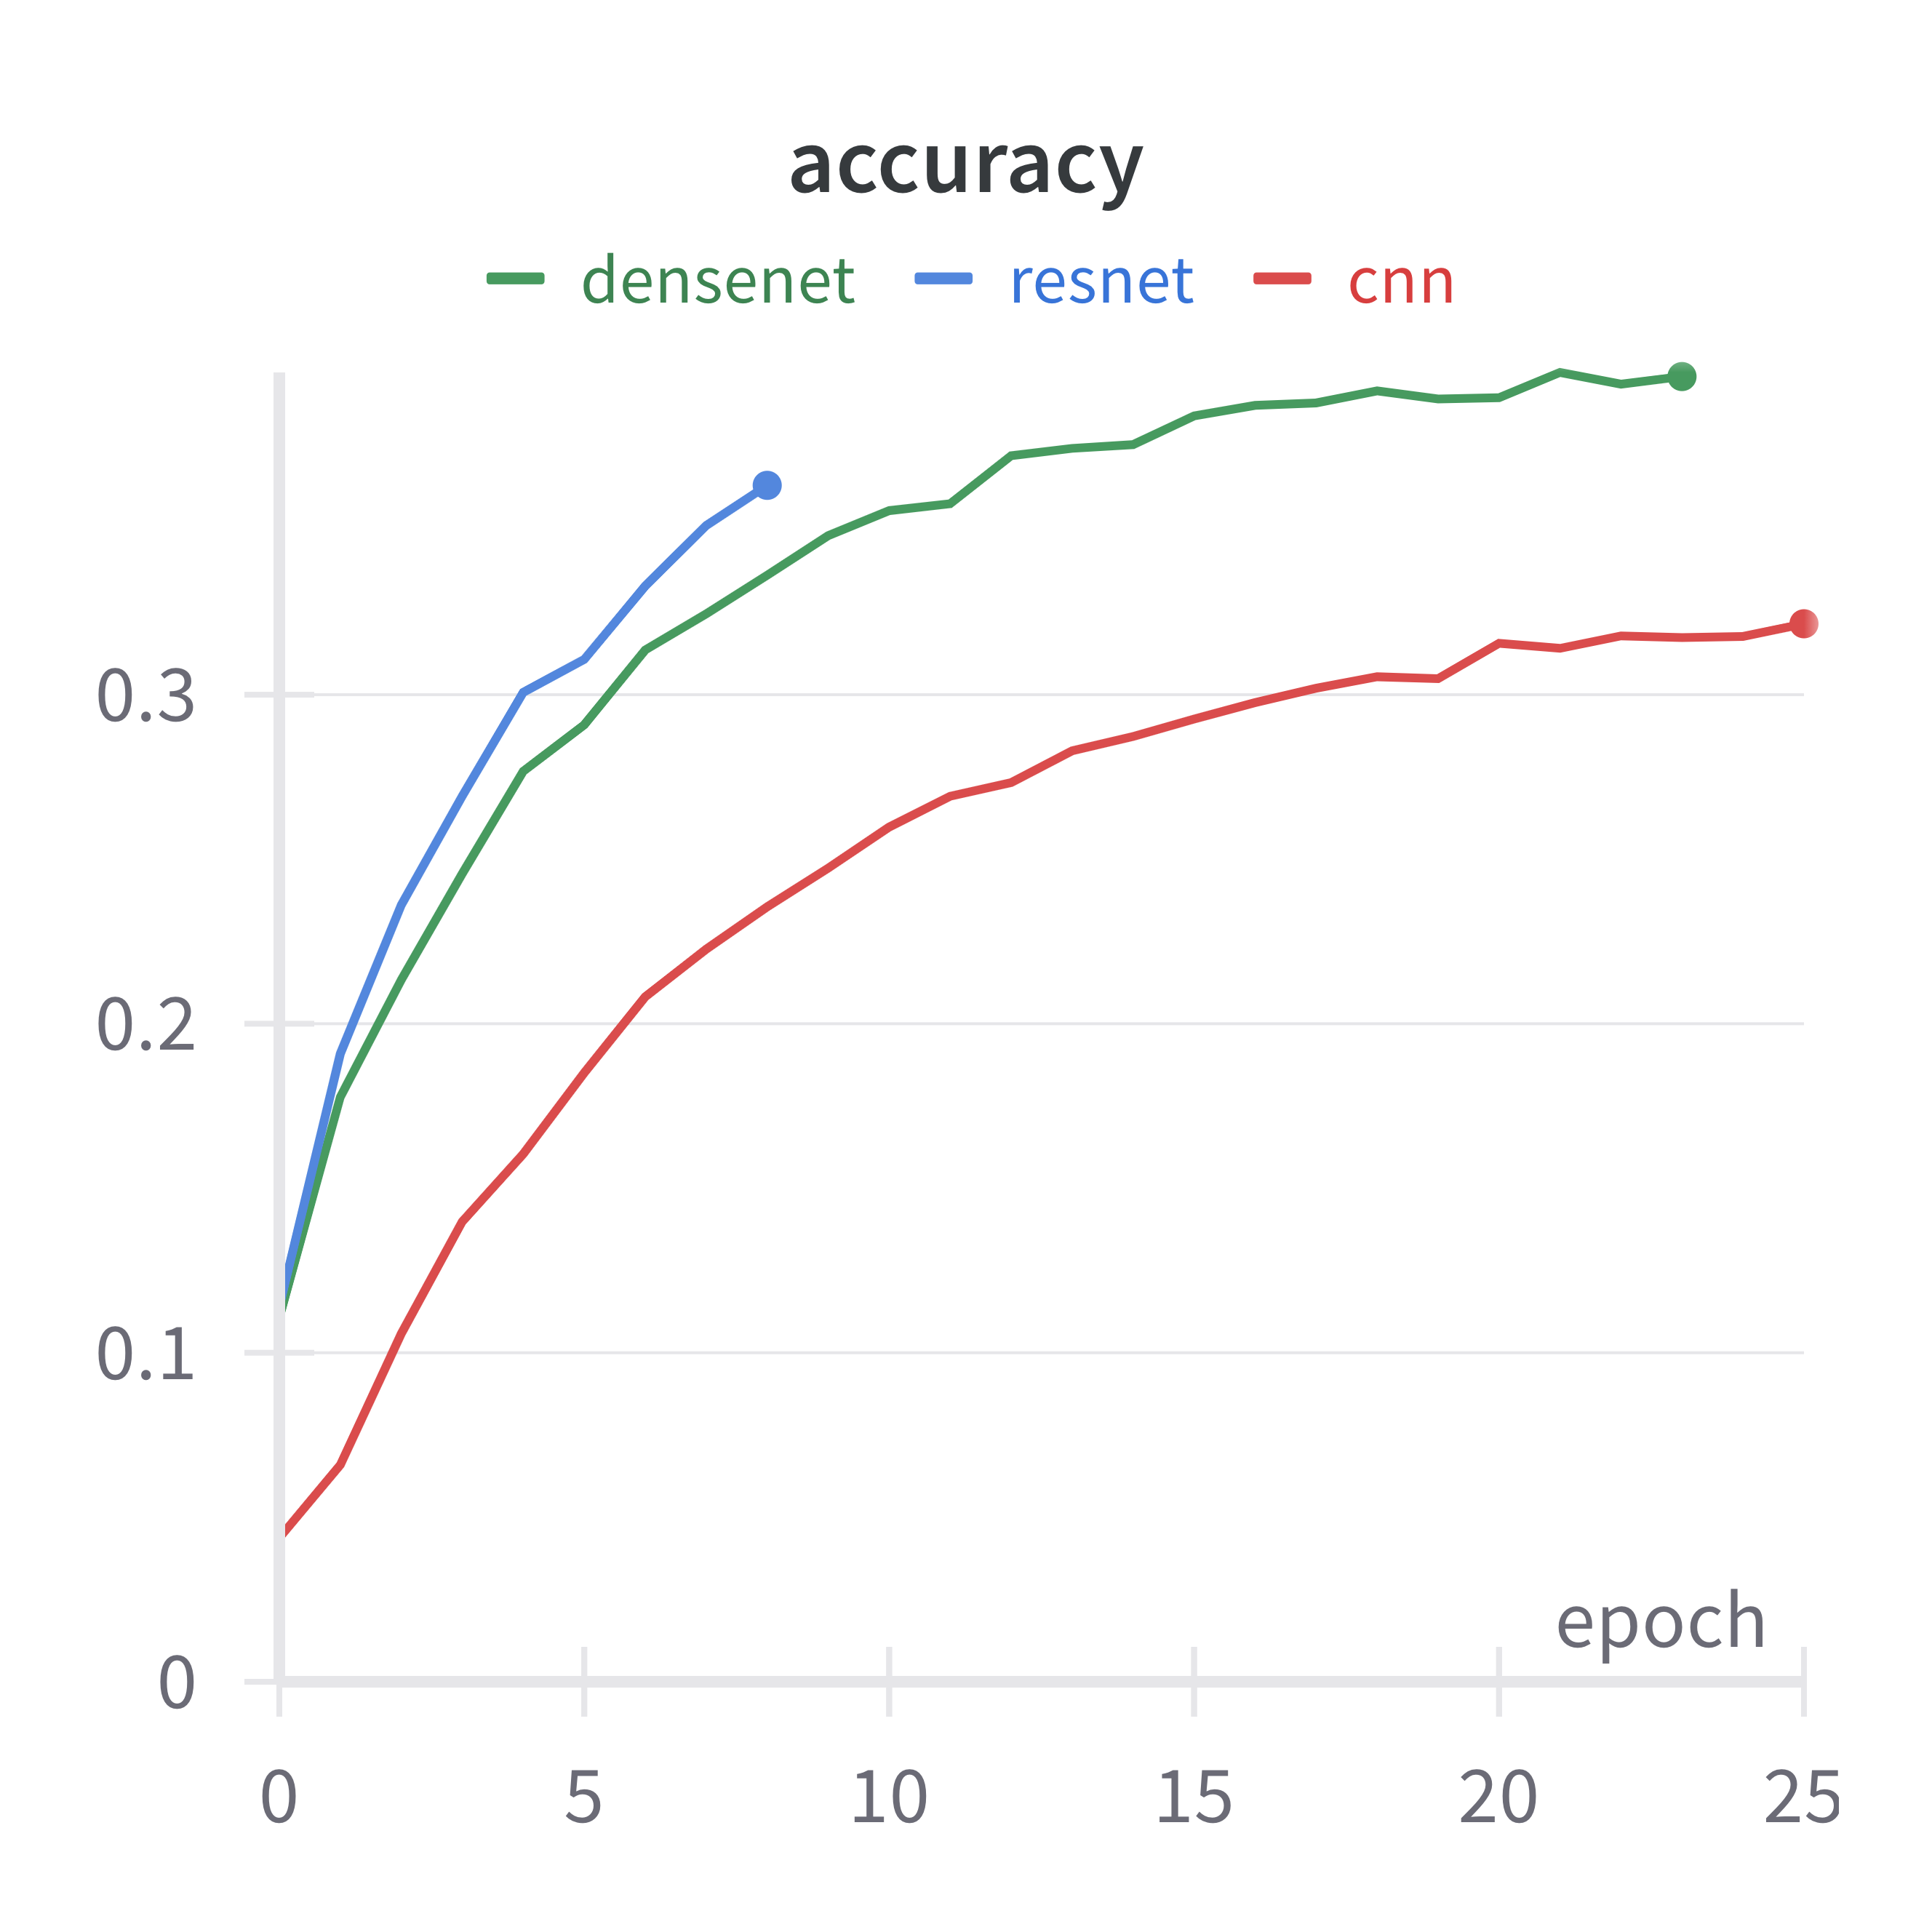
\includegraphics[width = 0.99 \textwidth]{images/205classes_accuracy.png}
        \caption{Accuracy}
    \end{subfigure}
    
    \caption{Performances of the convolutional architectures on the full dataset \textit{Places}}
    \label{fig:205_convnets}
\end{figure}

In order to improve the performances and better suits the robotic application, the new version of the "17 dataset" was introduced. The losses and accuracies of the different architectures are shown on Fig. \ref{fig:17_convnets}

\begin{figure}[H]
    \centering
    \begin{subfigure}{0.235 \textwidth}
        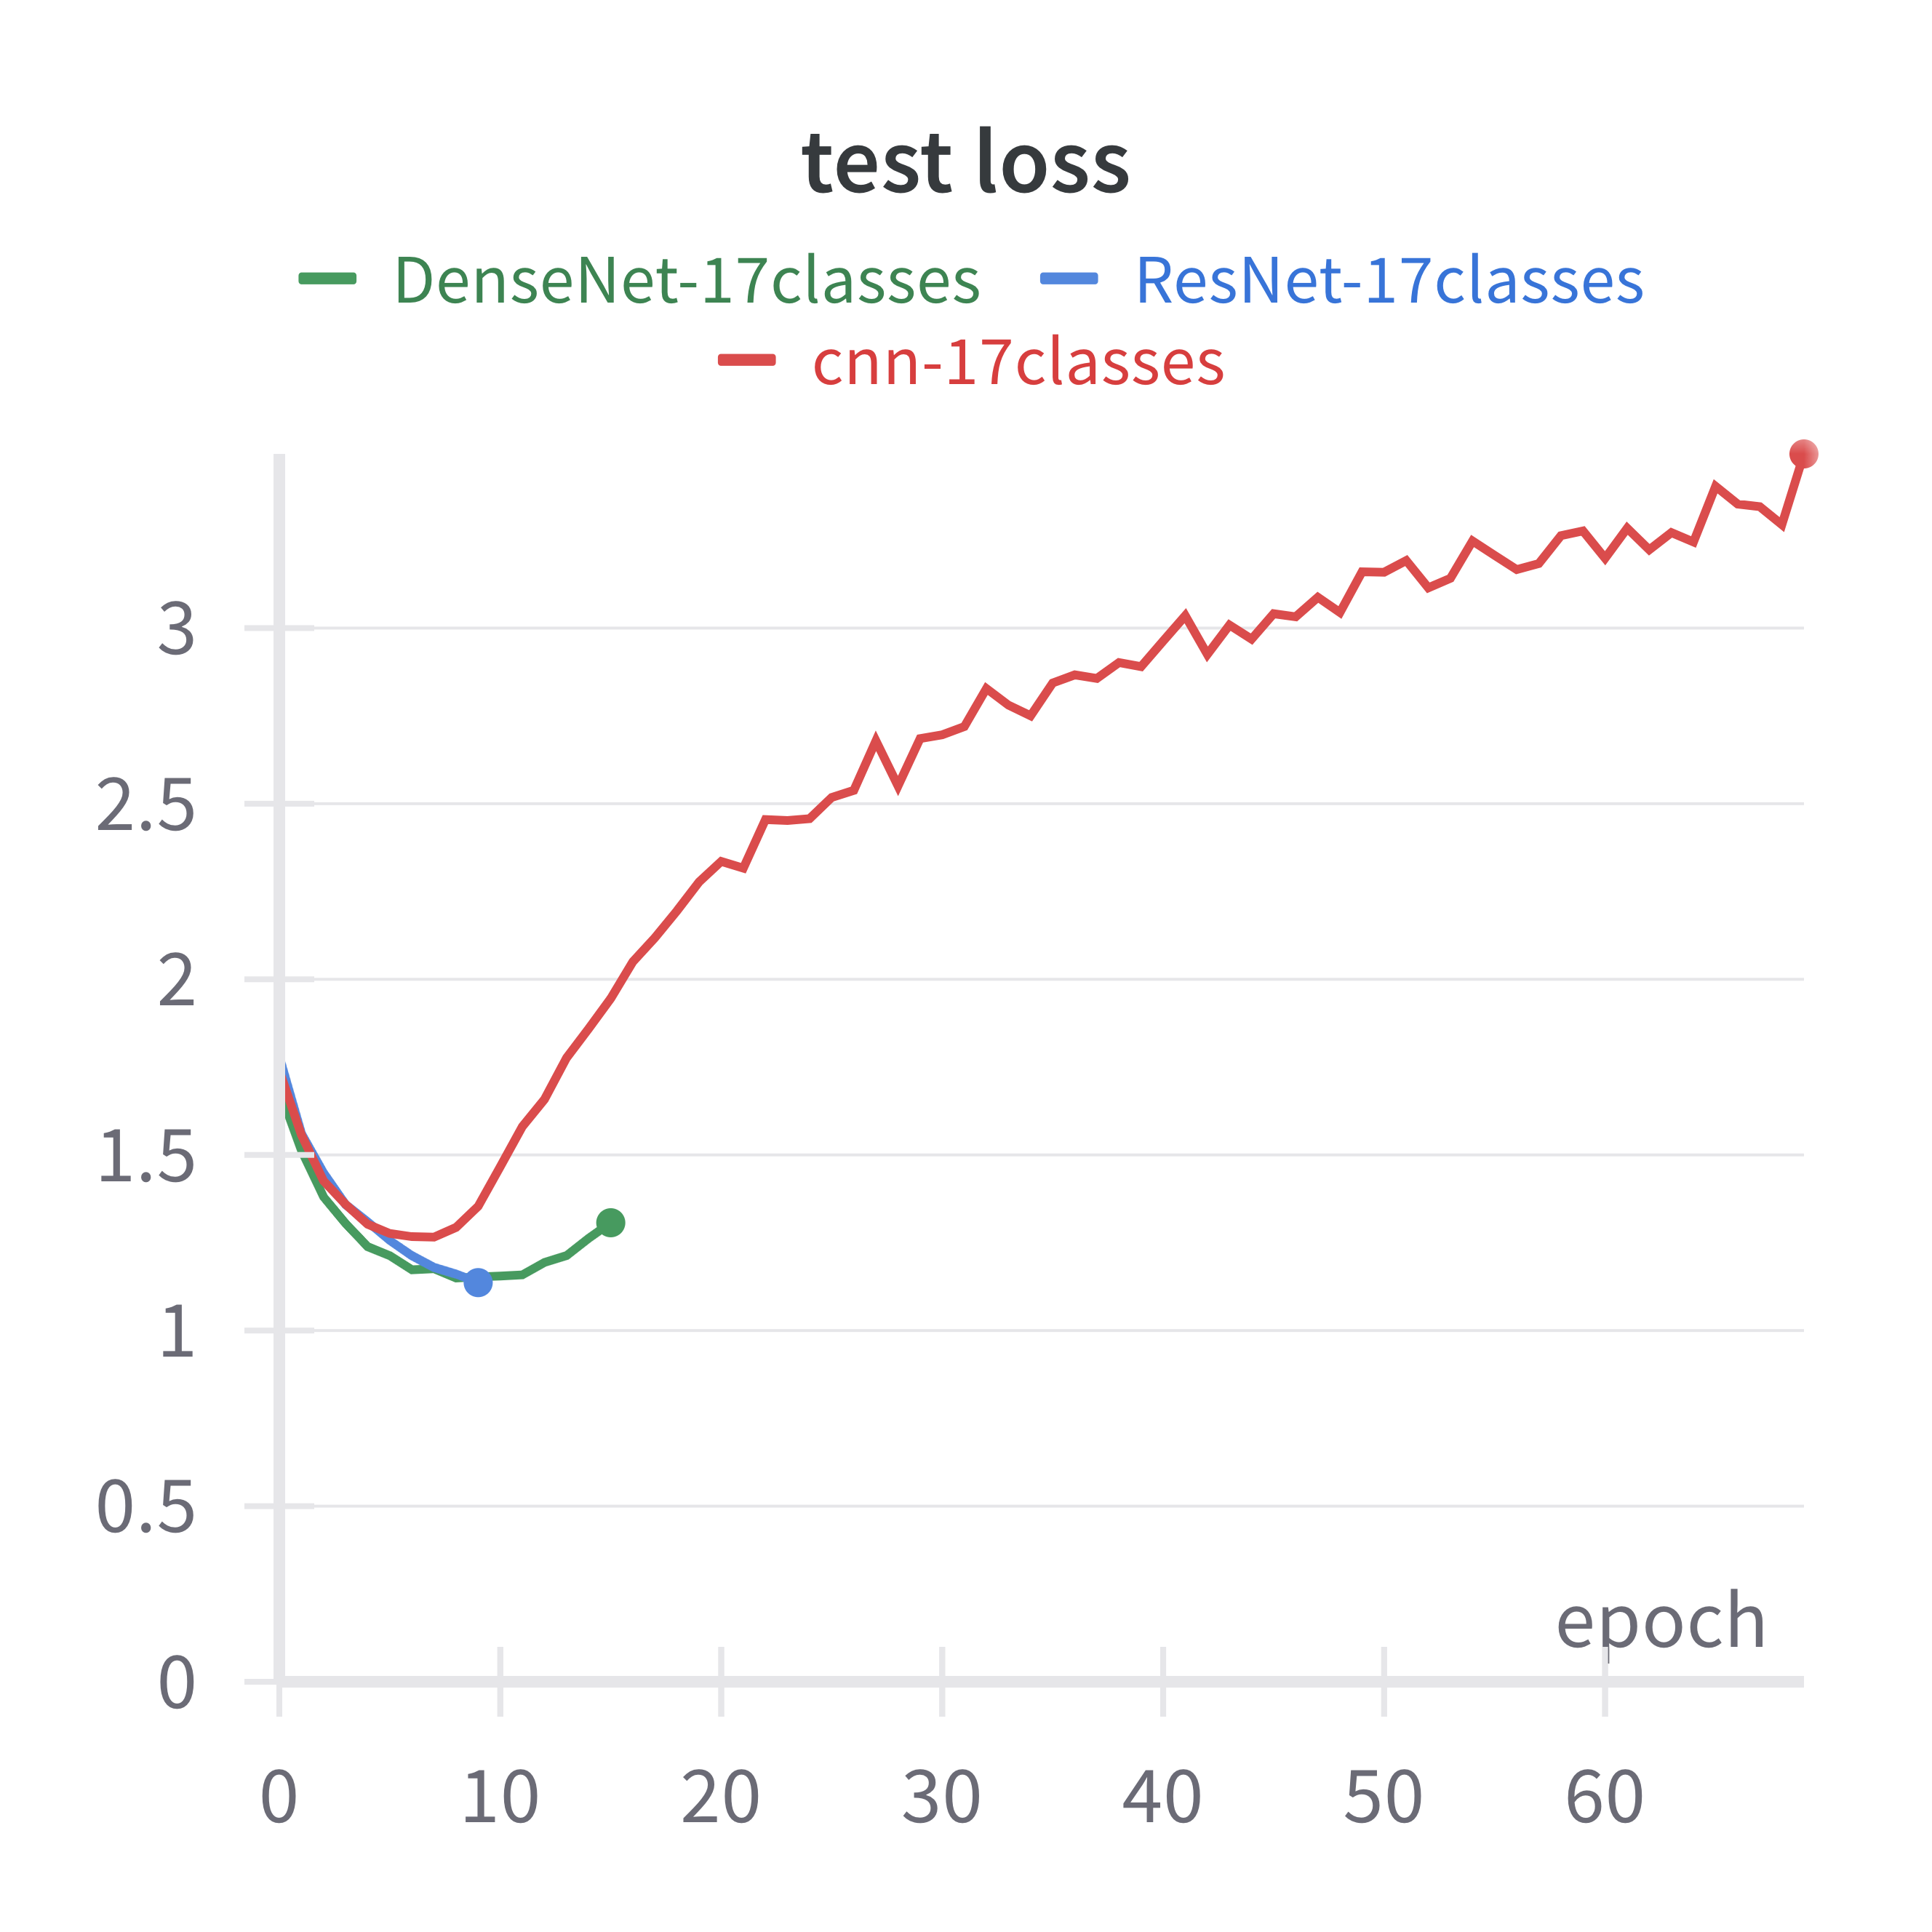
\includegraphics[width = 0.99 \textwidth]{images/17classes_test.png}
        \caption{Test Loss}
    \end{subfigure}
    \begin{subfigure}{0.235 \textwidth}
        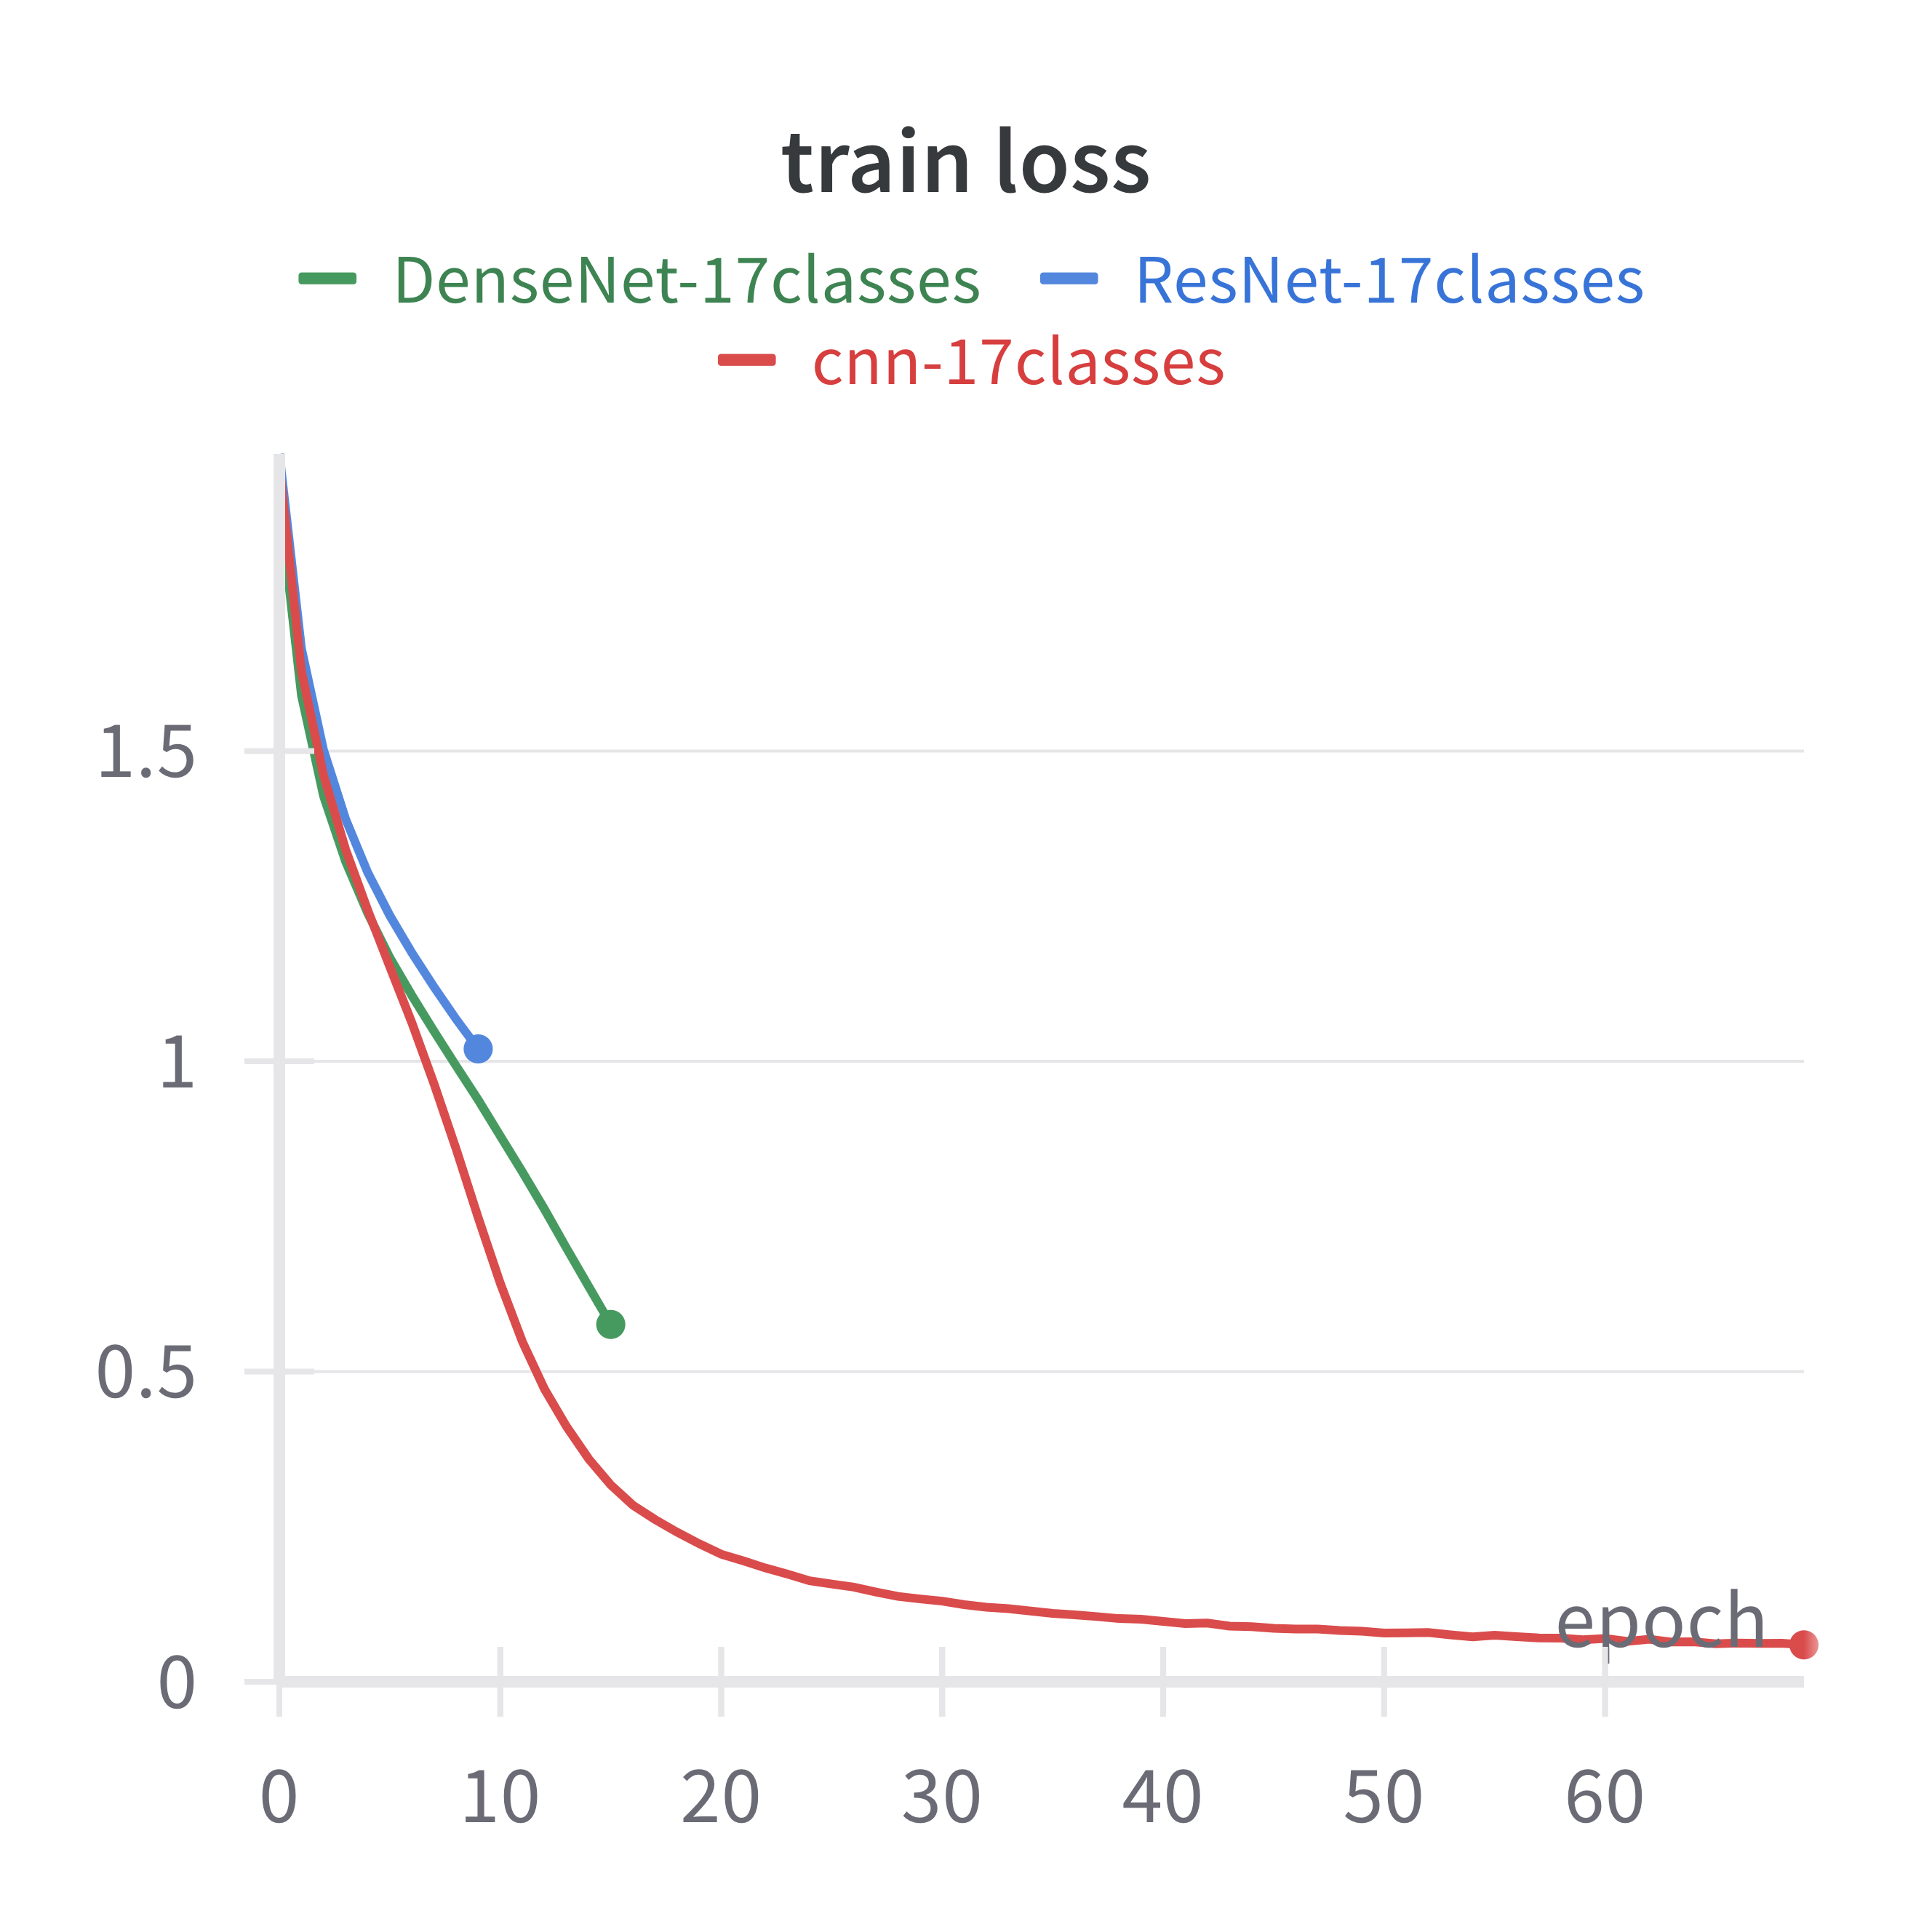
\includegraphics[width = 0.99 \textwidth]{images/17classes_train.png}
        \caption{Train Loss}
    \end{subfigure}
    \begin{subfigure}{0.35 \textwidth}
        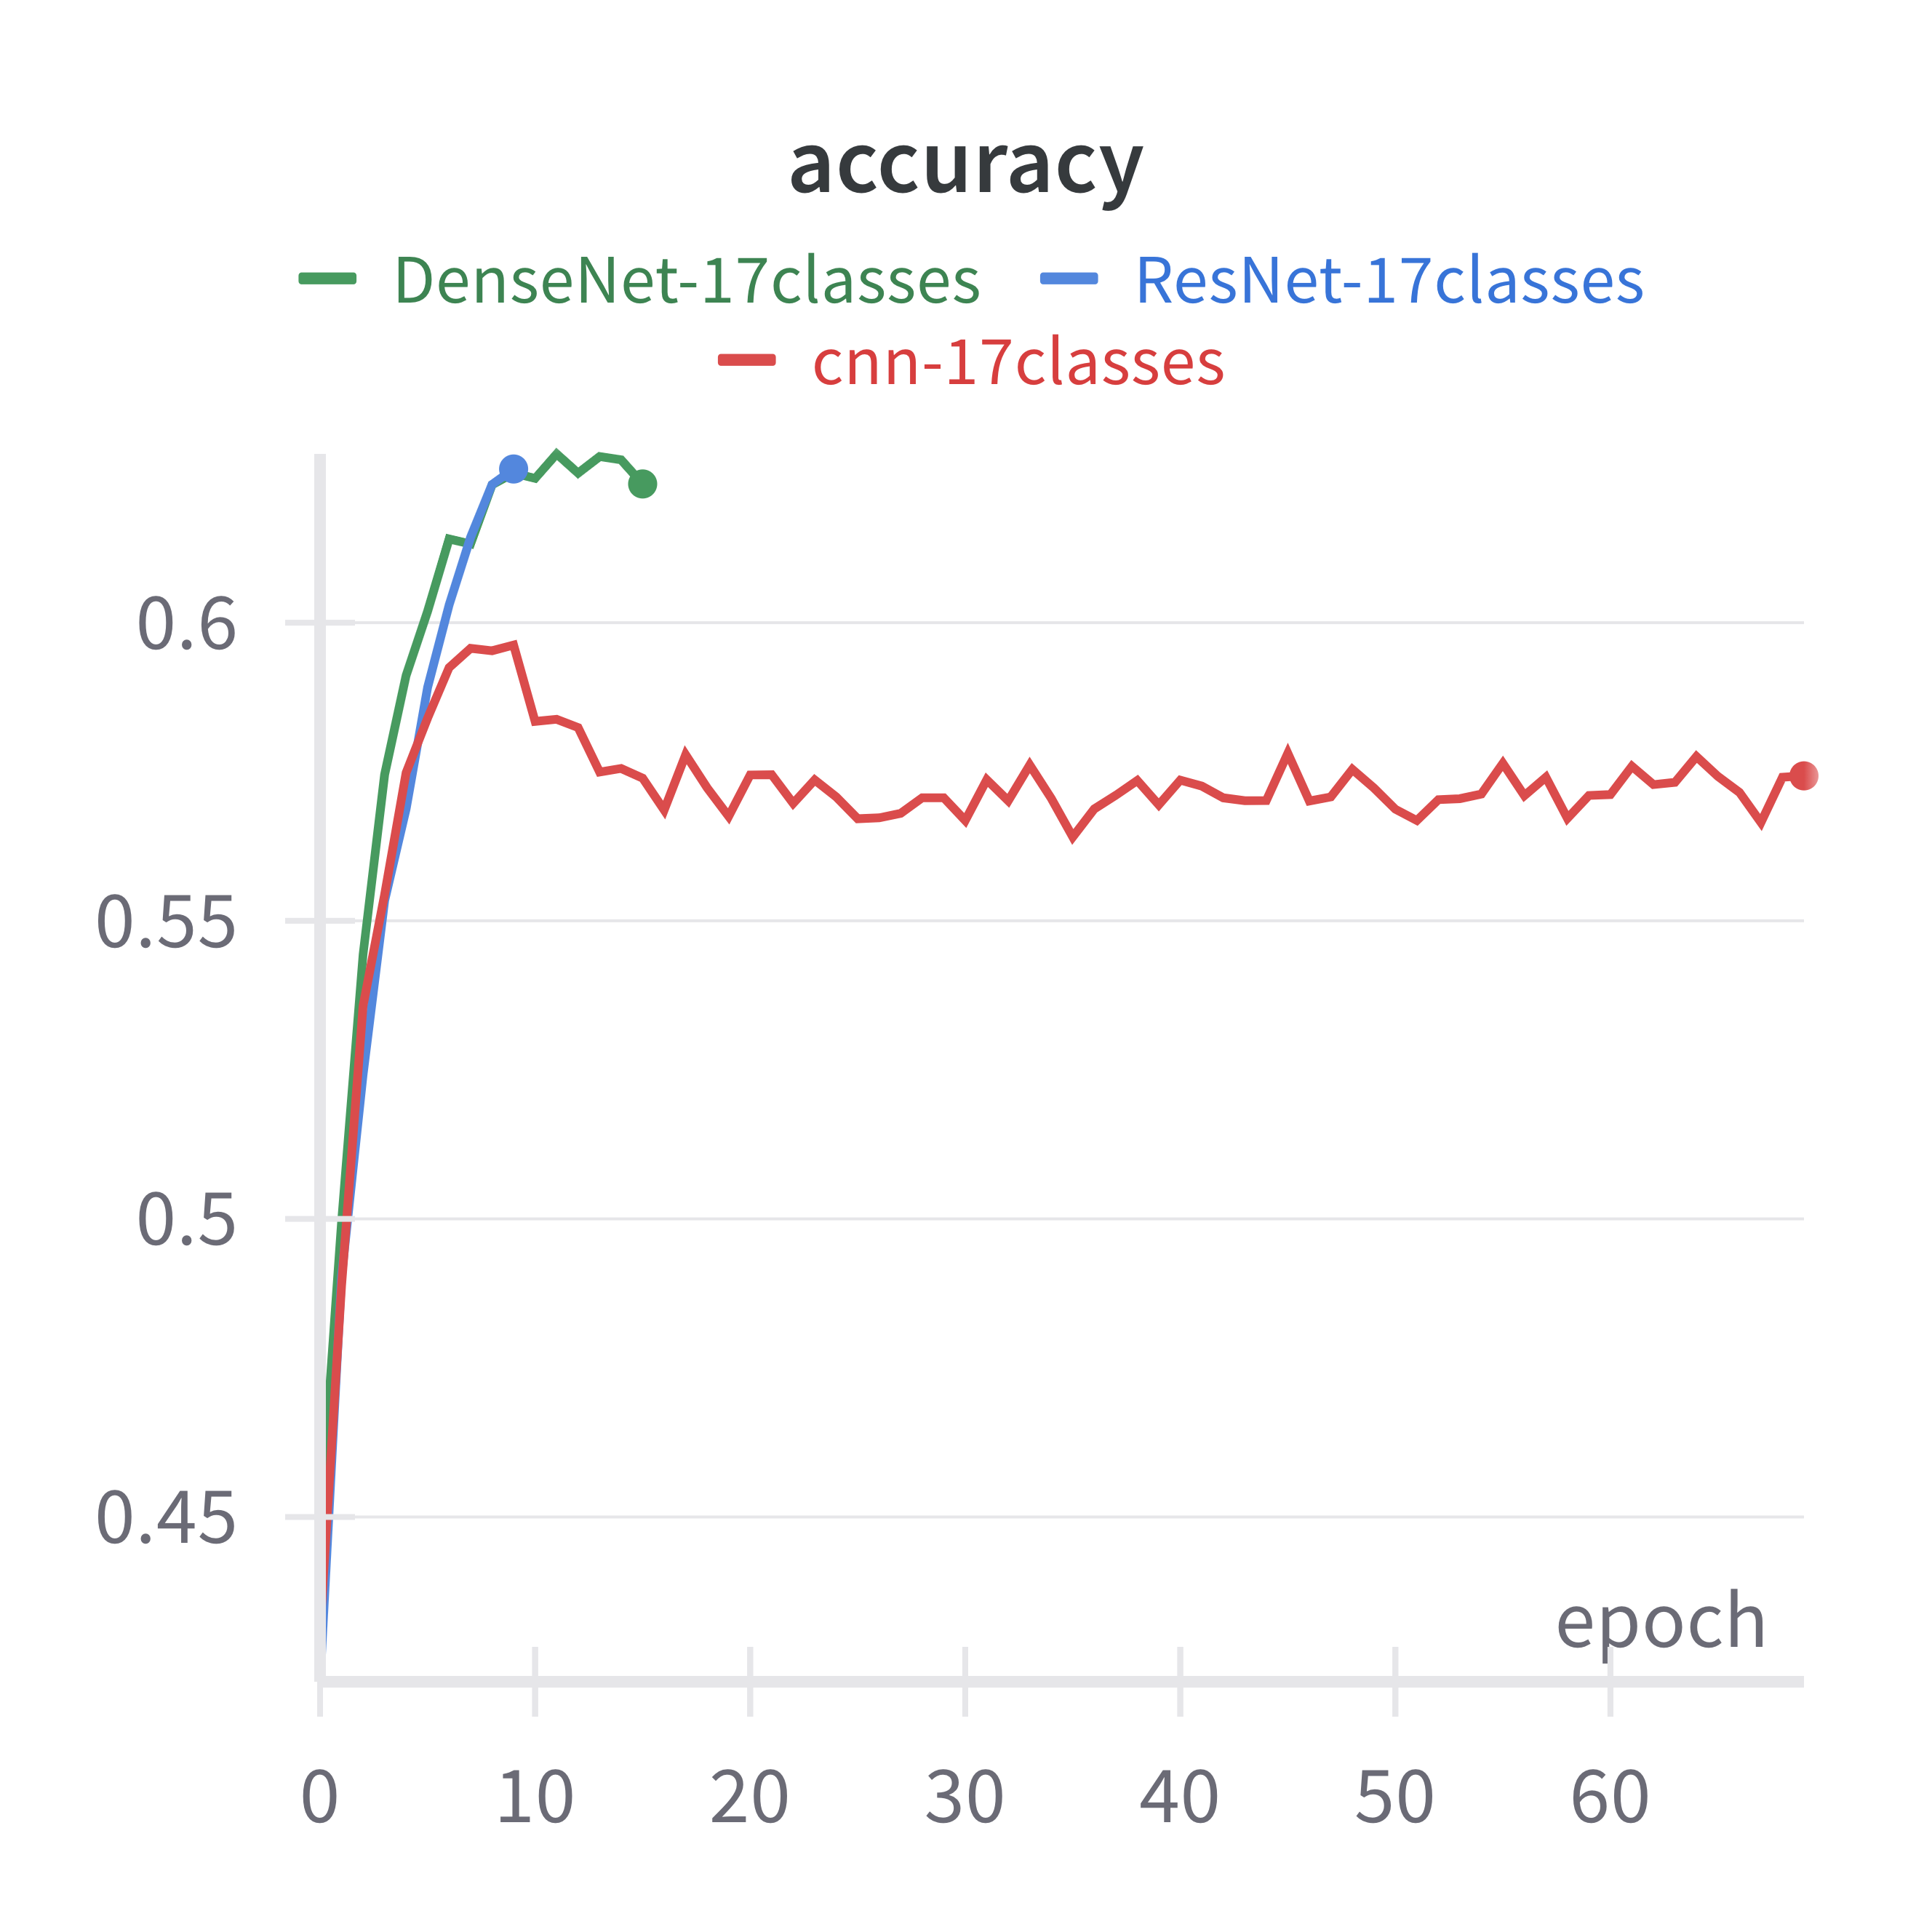
\includegraphics[width = 0.99 \textwidth]{images/17classes_accuracy.png}
        \caption{Accuracy}
    \end{subfigure}
    
    \caption{Performances of the convolutional architectures on the condensed version of the \textit{Places} dataset}
    \label{fig:17_convnets}
\end{figure}

The behavior is quite similar to the previous observation: ResNet and DenseNet outperform ConvNet, with ResNet not having enough time to reach its maximum performance, while DenseNet appears to do so. However, a notable difference is the increase in scale: by relabeling the images and reducing the number of classes, the maximum accuracy has been mulitplied by a factor greater than 1.5. Additionally, the output labels are now more aligned with the application, providing a total benefit.\\

\subsubsection{Visual Transformer}

Given the lengthy training time required for this final architecture, two versions were trained:

\begin{itemize}
    \setlength{\itemsep}{1mm}
    \item [$\bullet$] \textbf{A larger version} with approximately 600K parameters, which was unable to complete more than 3 epochs within the maximal training time allowed (the same as for the \textit{IntelImages} dataset). 
    \item [$\bullet$] \textbf{A scaled-down version} of the previous architecture, with around 100K parameters, enabling the generation of more results for analysis.
\end{itemize}



\begin{figure}[H]
    \centering
    \begin{subfigure}{0.235 \textwidth}
        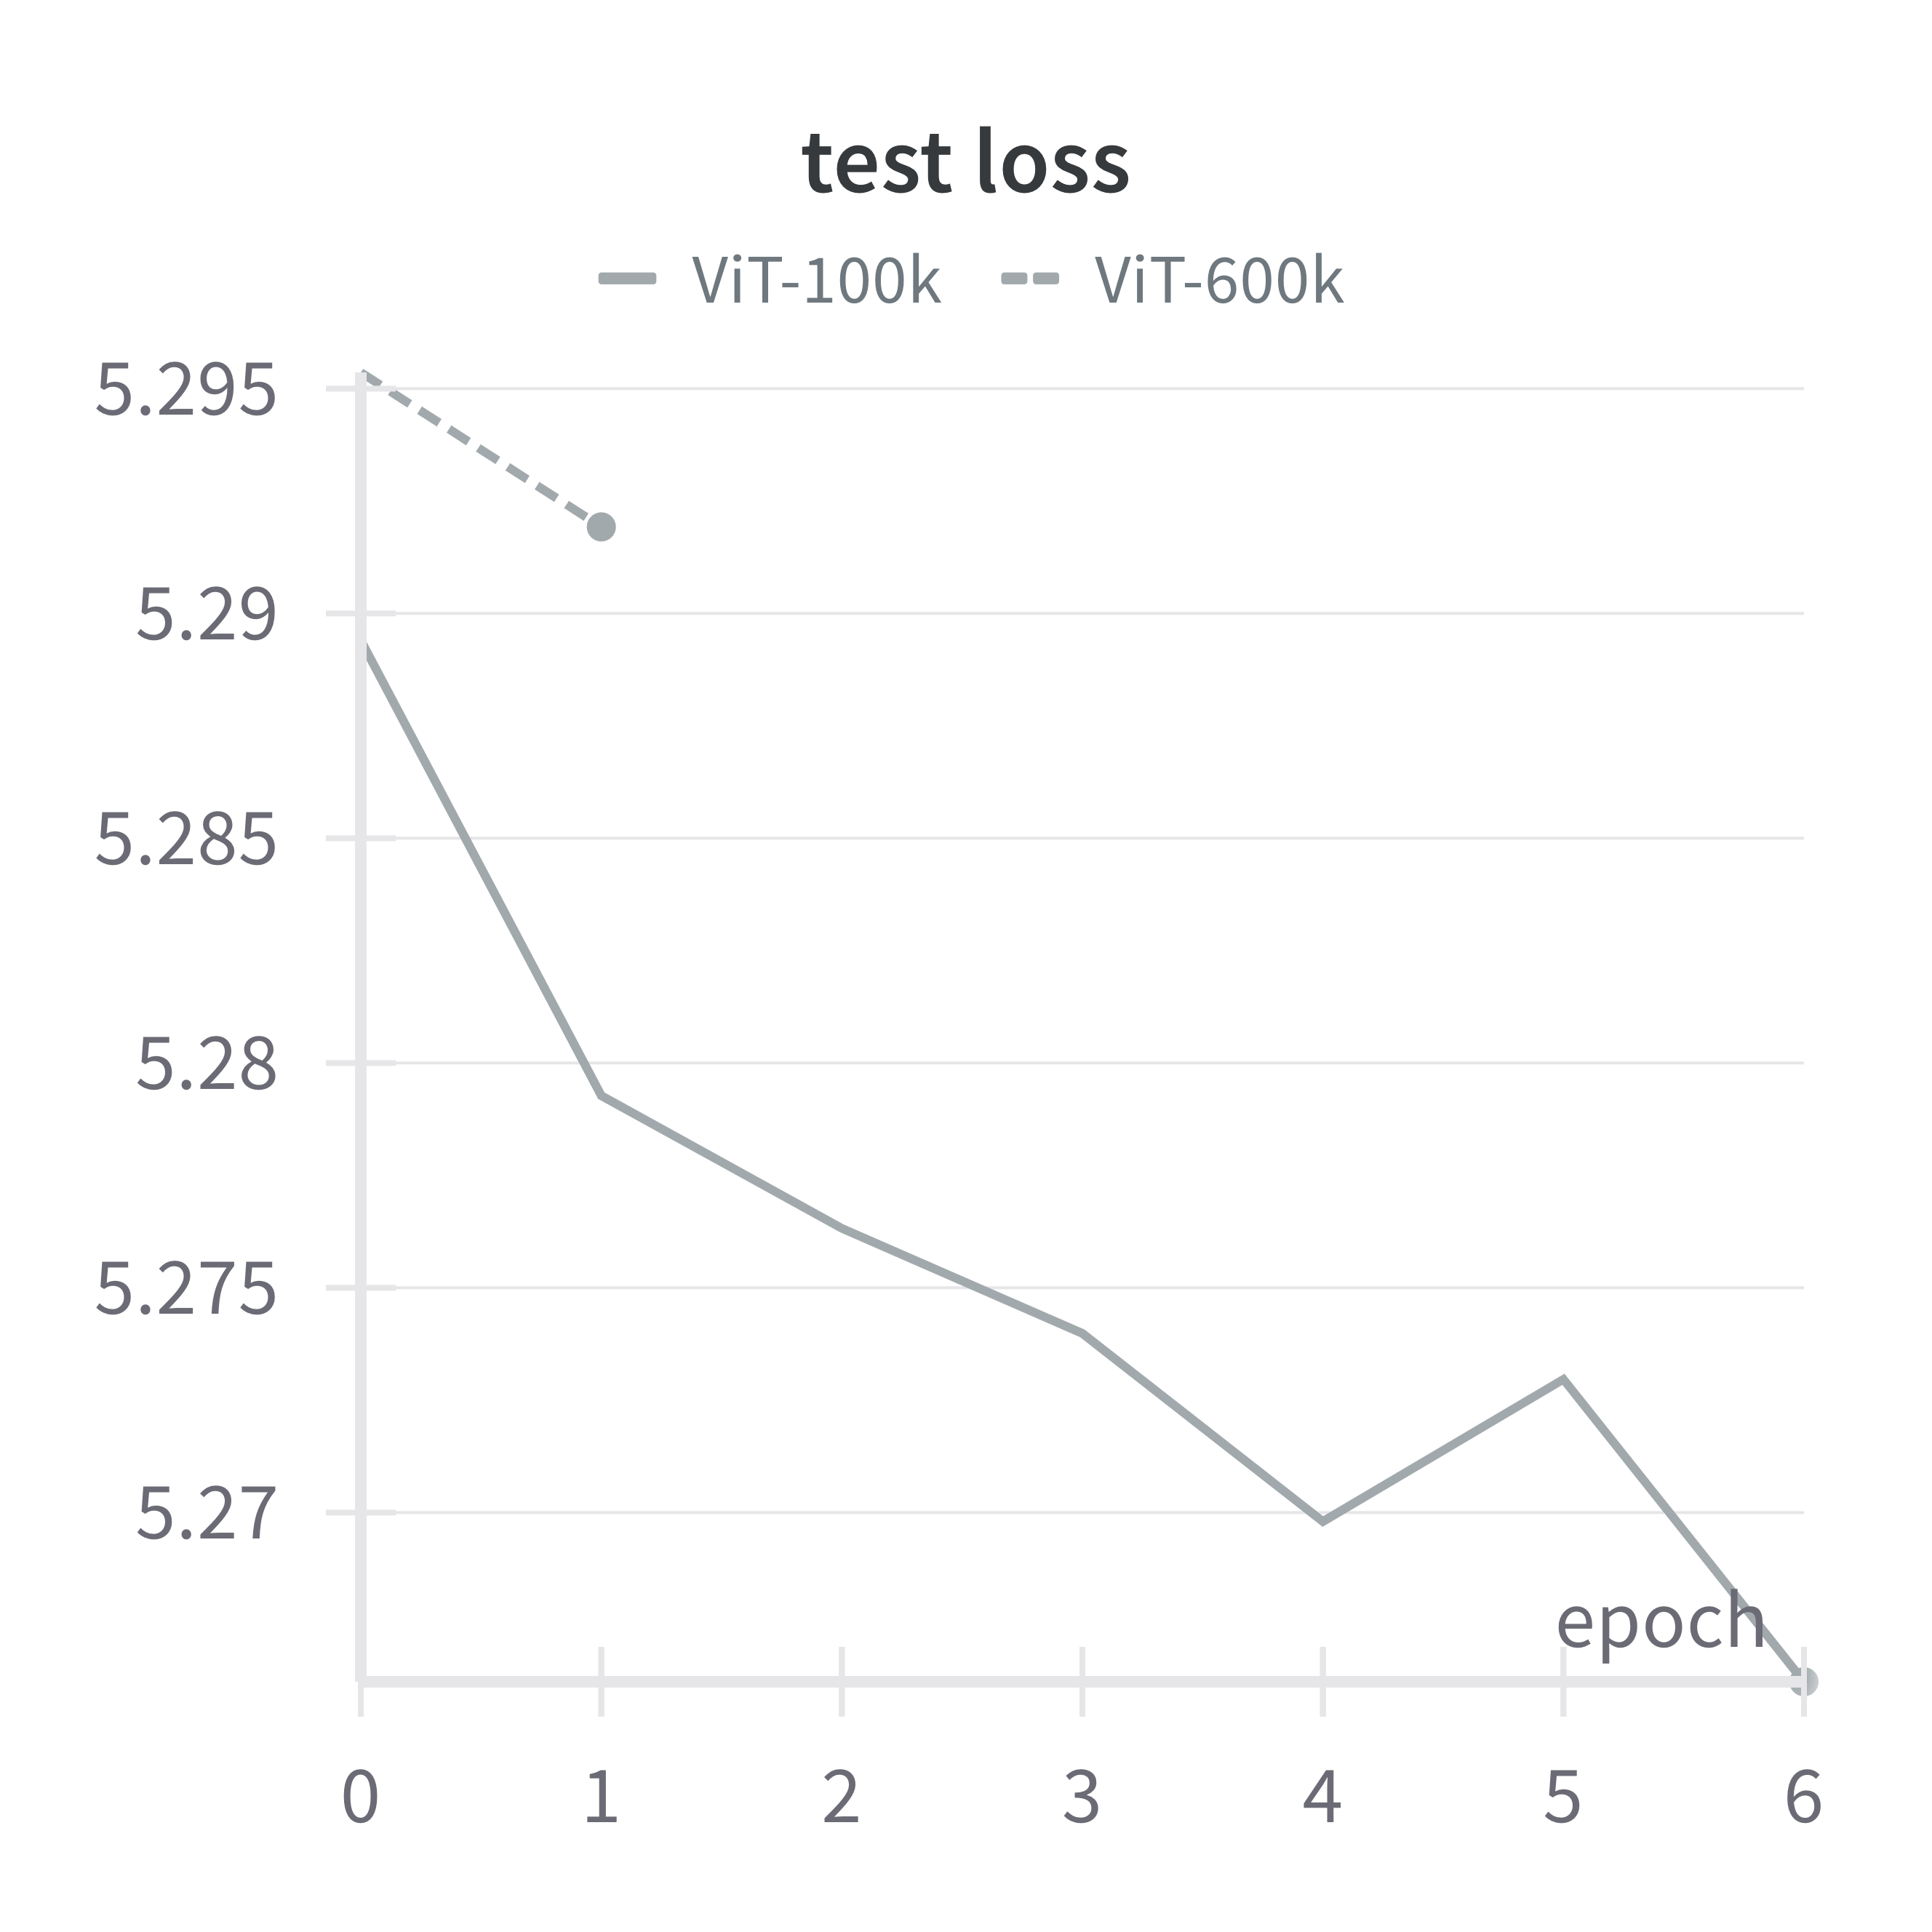
\includegraphics[width = 0.99 \textwidth]{images/205classes_vit_test.png}
        \caption{Test Loss}
    \end{subfigure}
    \begin{subfigure}{0.235 \textwidth}
        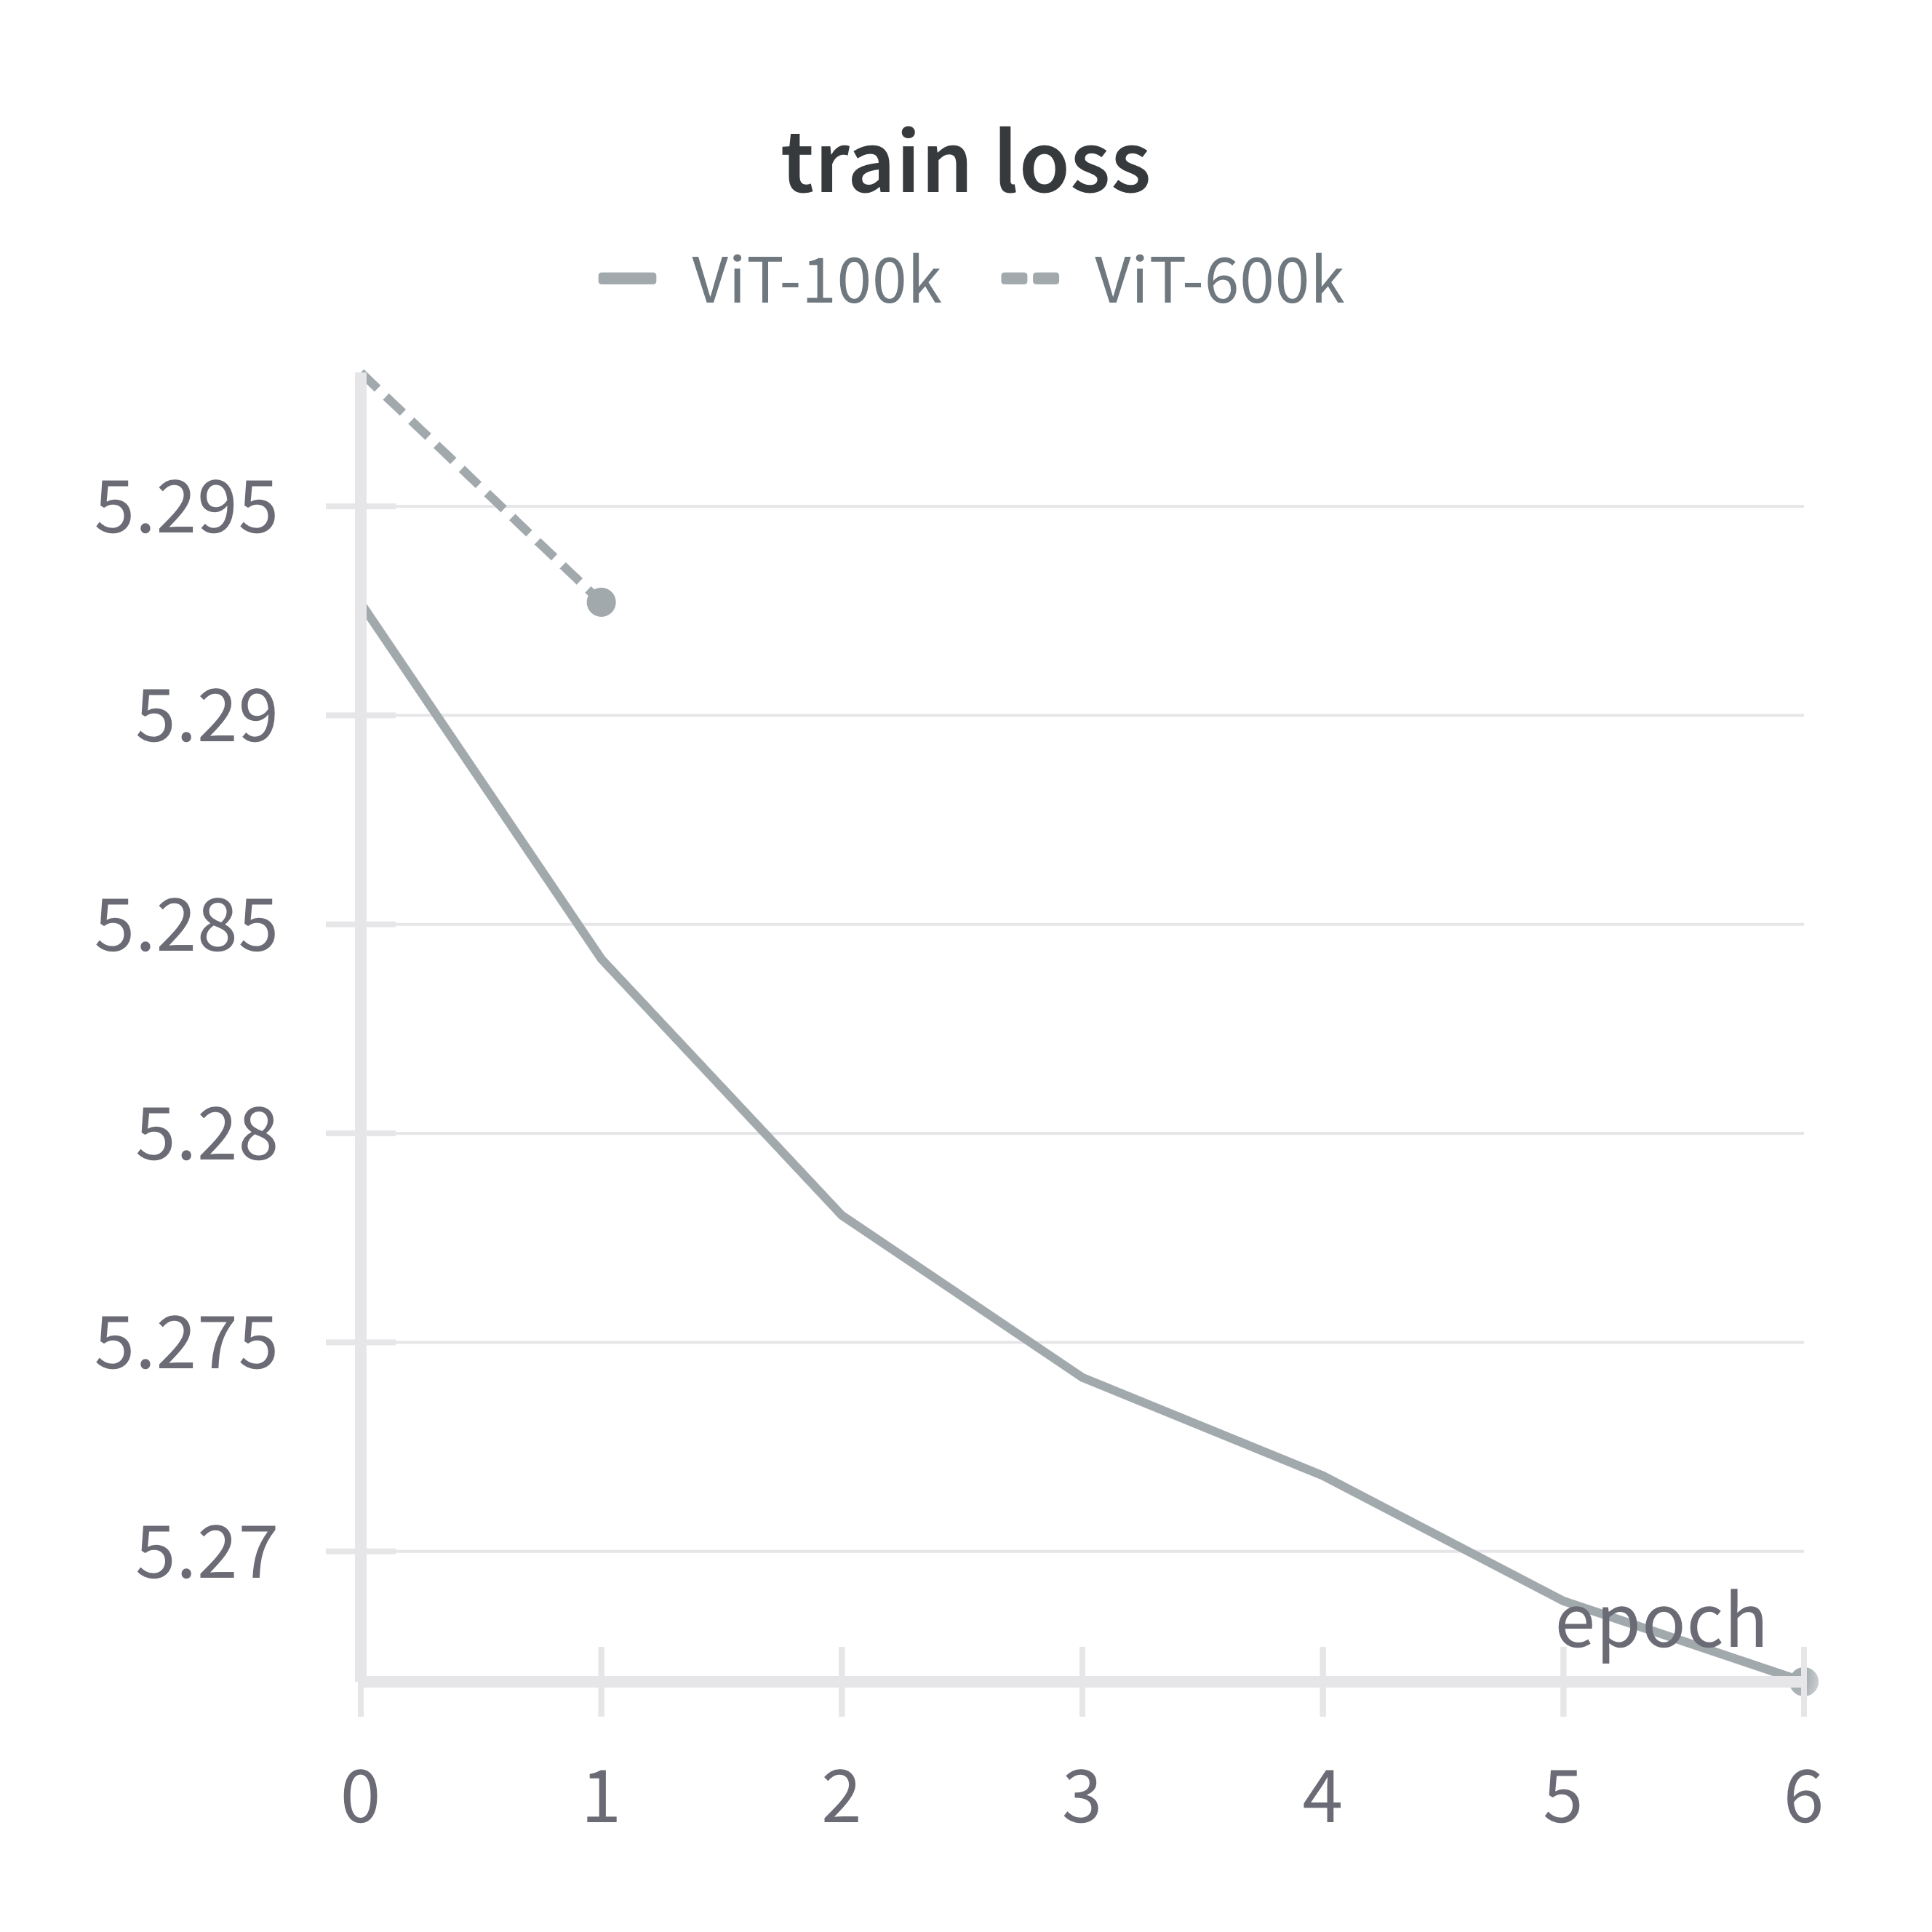
\includegraphics[width = 0.99 \textwidth]{images/205classes_vit_train.png}
        \caption{Train Loss}
    \end{subfigure}
    \begin{subfigure}{0.35 \textwidth}
        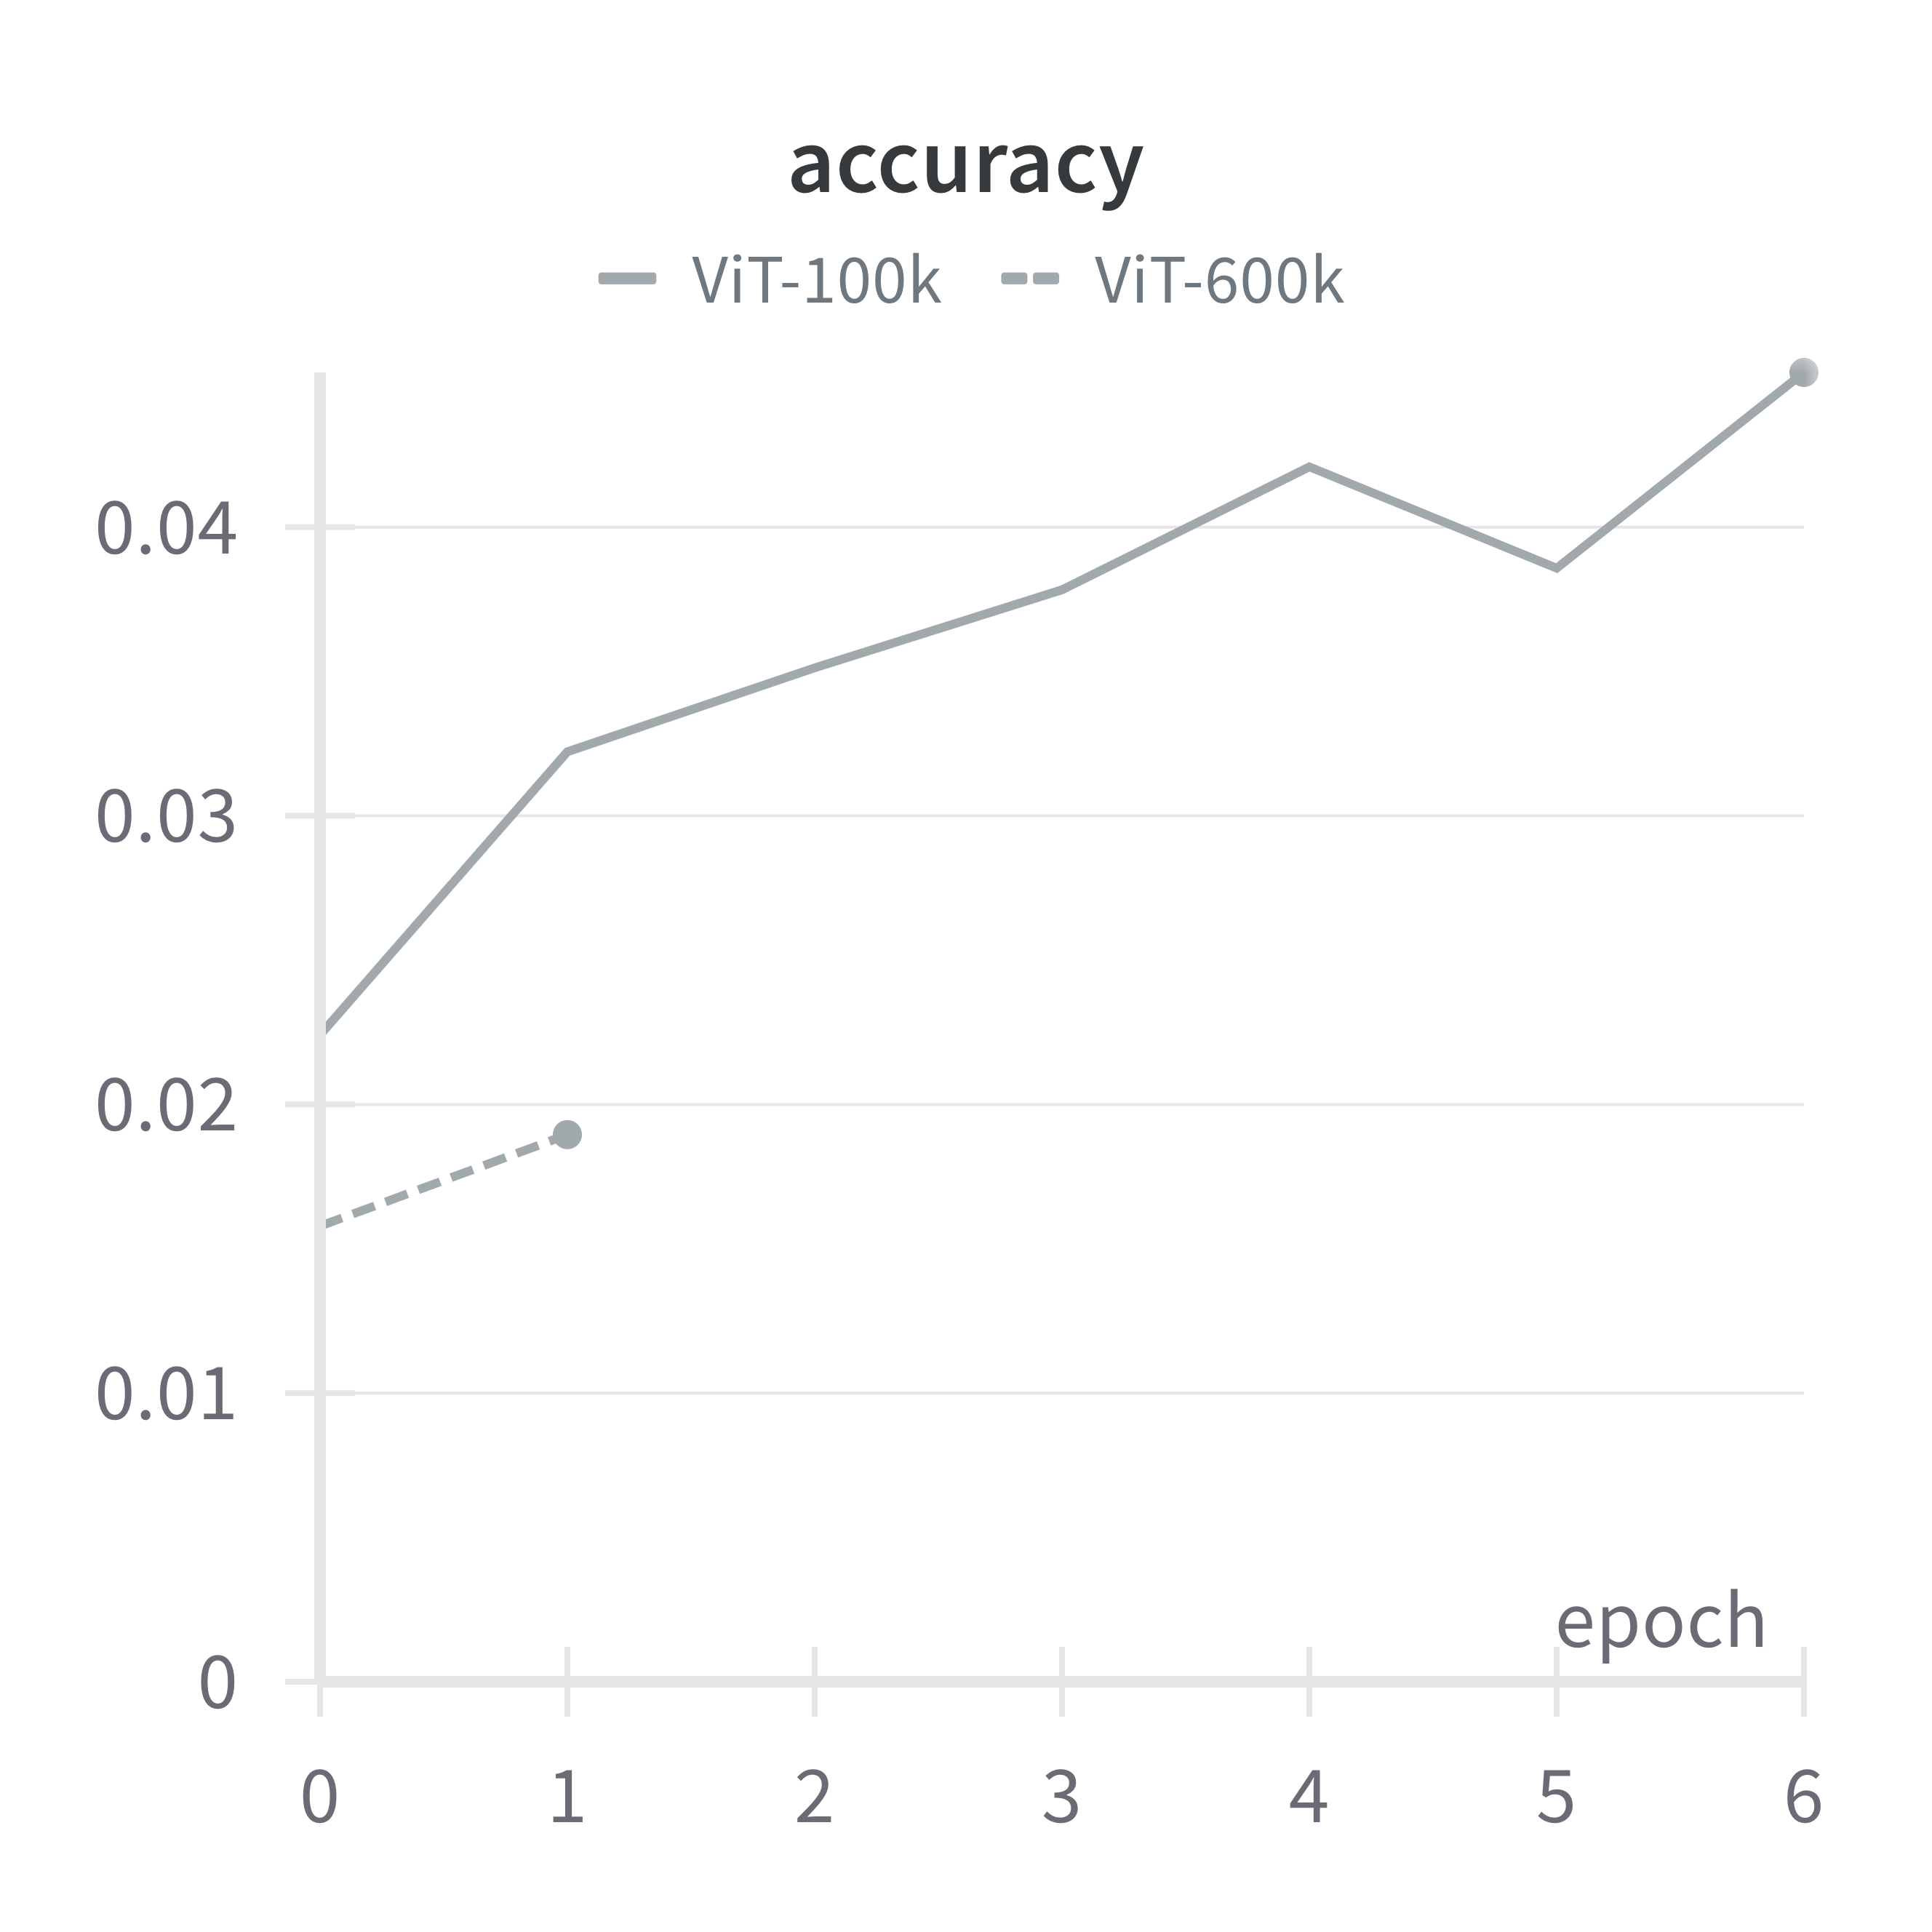
\includegraphics[width = 0.99 \textwidth]{images/205classes_vit_accuracy.png}
        \caption{Accuracy}
    \end{subfigure}
    
    \caption{Performances of two versions of the visual transformer on the full \textit{Places} dataset}
    \label{fig:205_vit}
\end{figure}

As already explained, the performances of the visual transformer are very bad as can be seen on \ref{fig:205_vit}, just above a full-random guess. But, one can see that the losses are decreasing and the accuracy increasing, what suggests that it could lead to good results if it was trained for a longer time. The same architectures have been trained on the condensed version of the dataset, the results being shown on Fig. \ref{fig:17_vit}. Due to a crash during training, it has not been possible to train the lighter model during the expected amount of time. But one can see that the results are already way better, highlighting the improvements brought by the relabeling of the dataset. 

\begin{figure}[H]
    \centering
    \begin{subfigure}{0.235 \textwidth}
        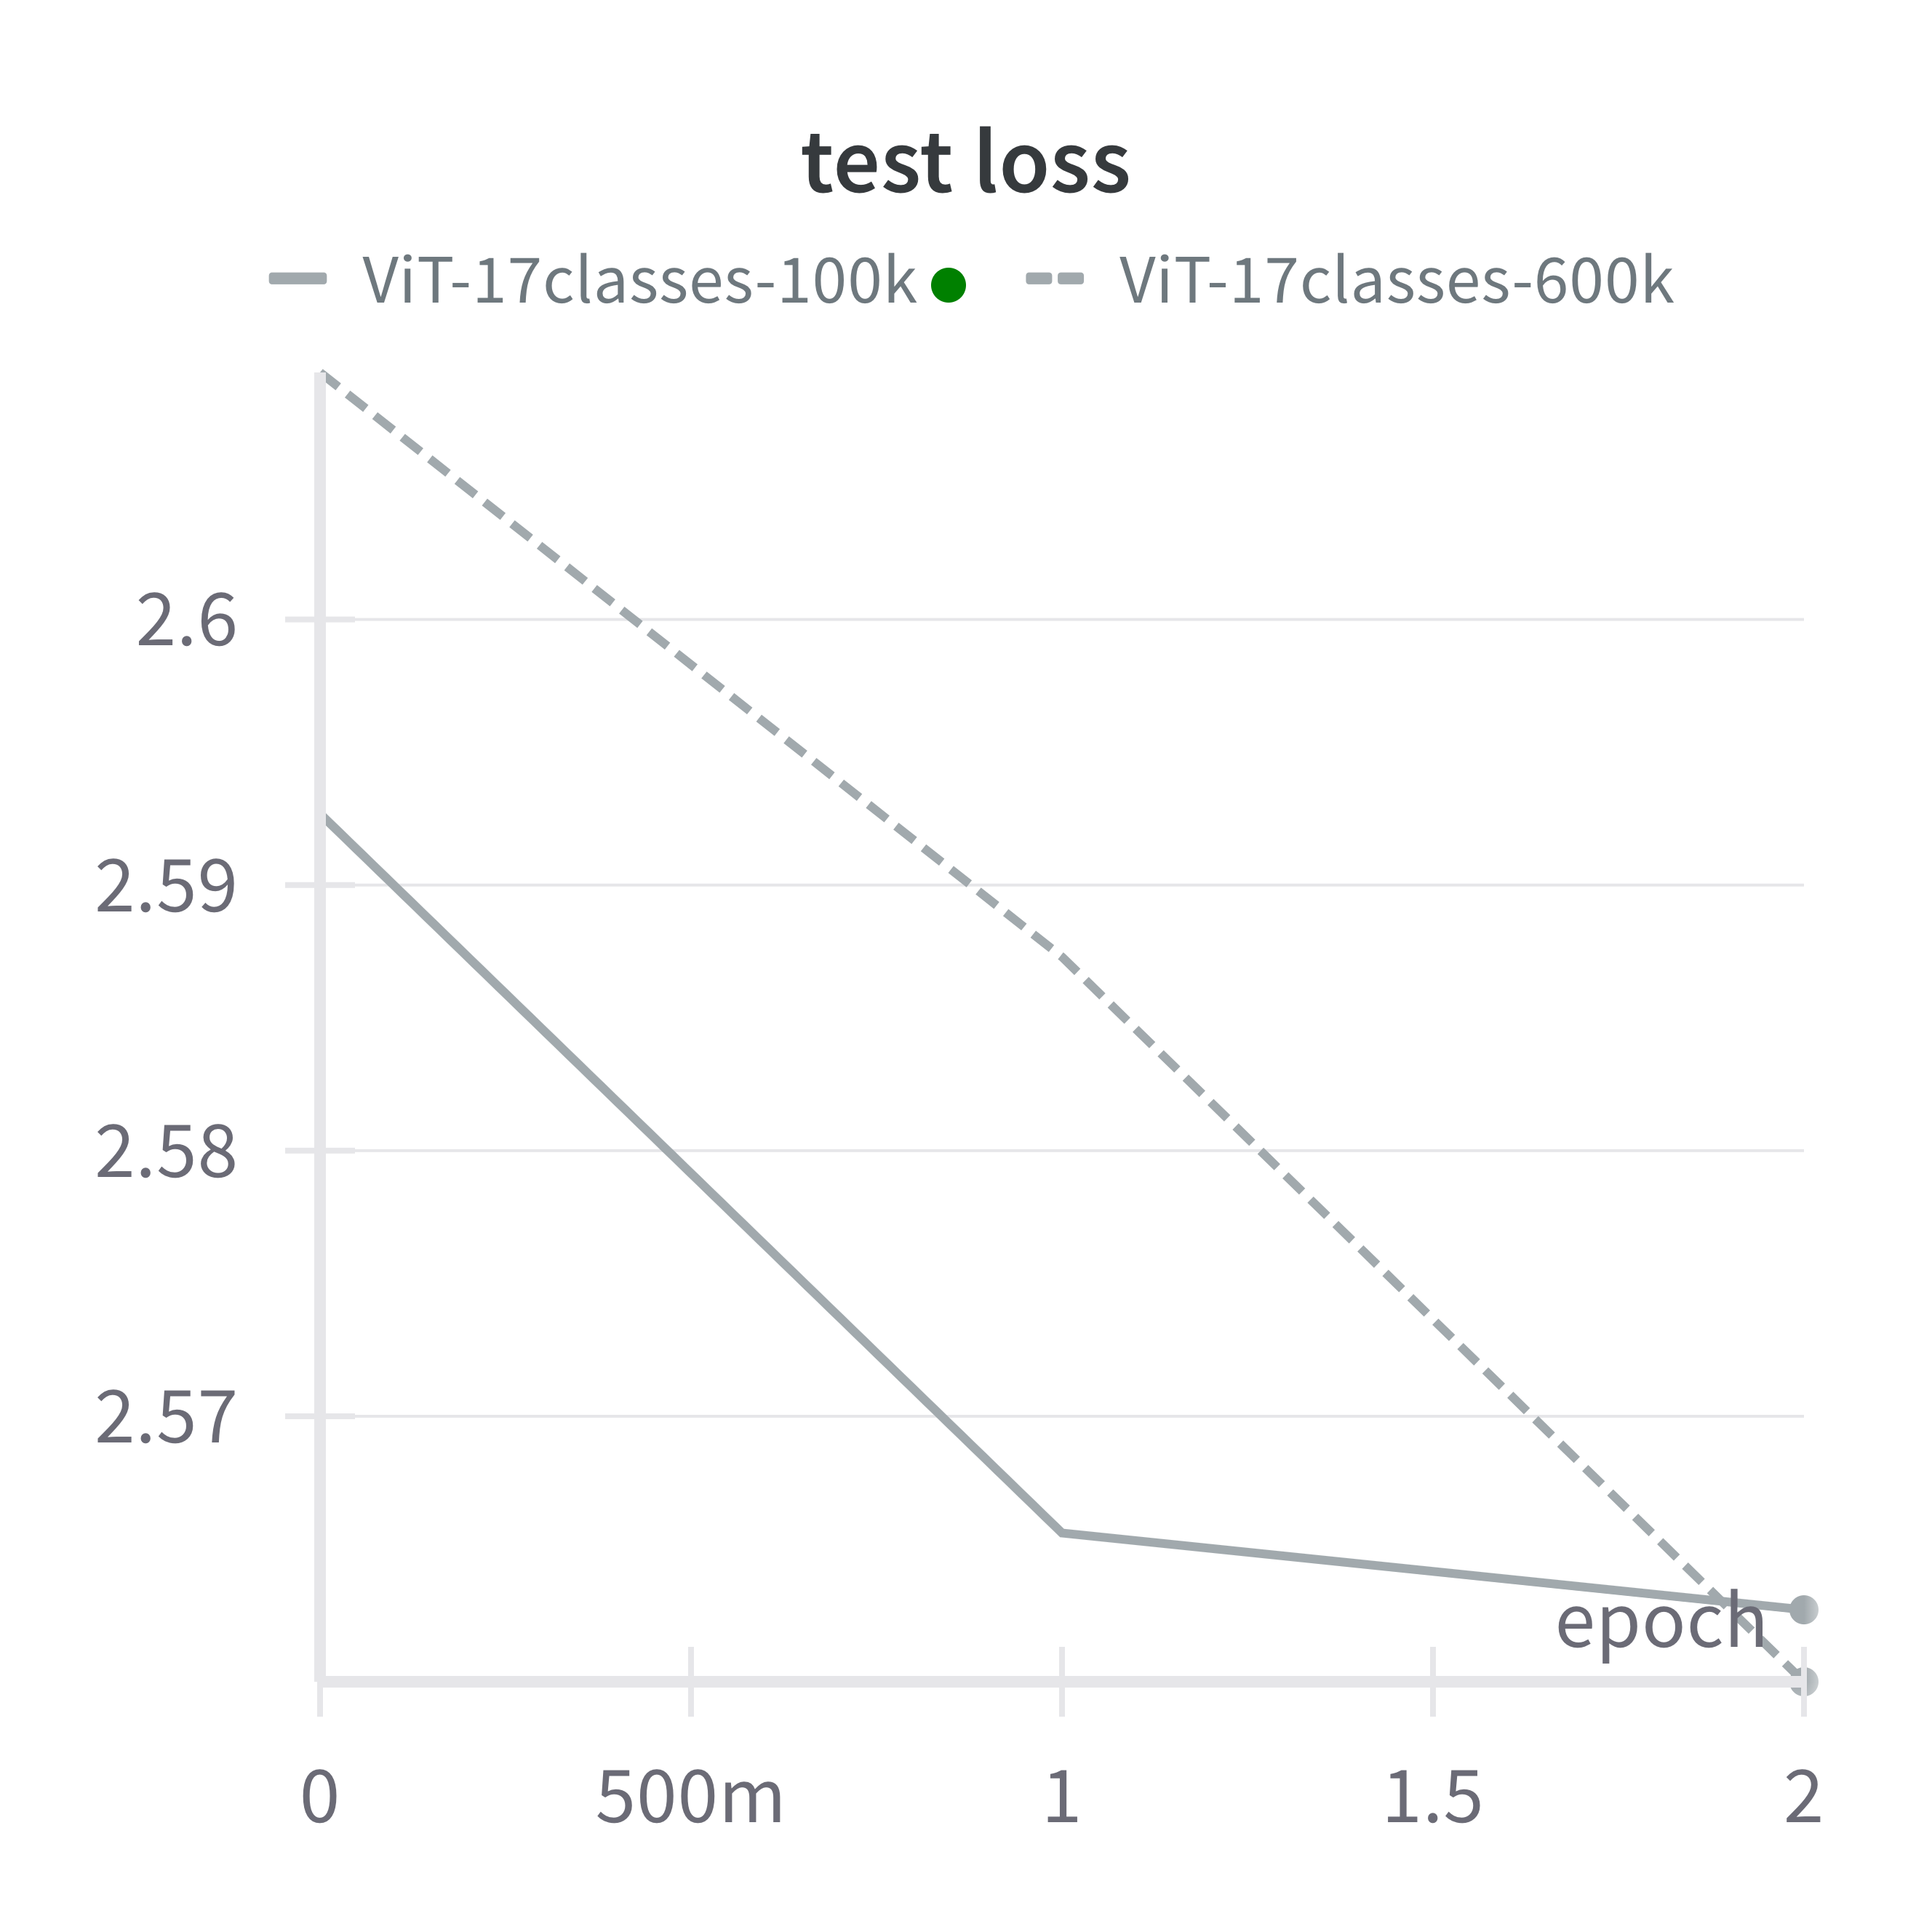
\includegraphics[width = 0.99 \textwidth]{images/17classes_vit_test.png}
        \caption{Test Loss}
    \end{subfigure}
    \begin{subfigure}{0.235 \textwidth}
        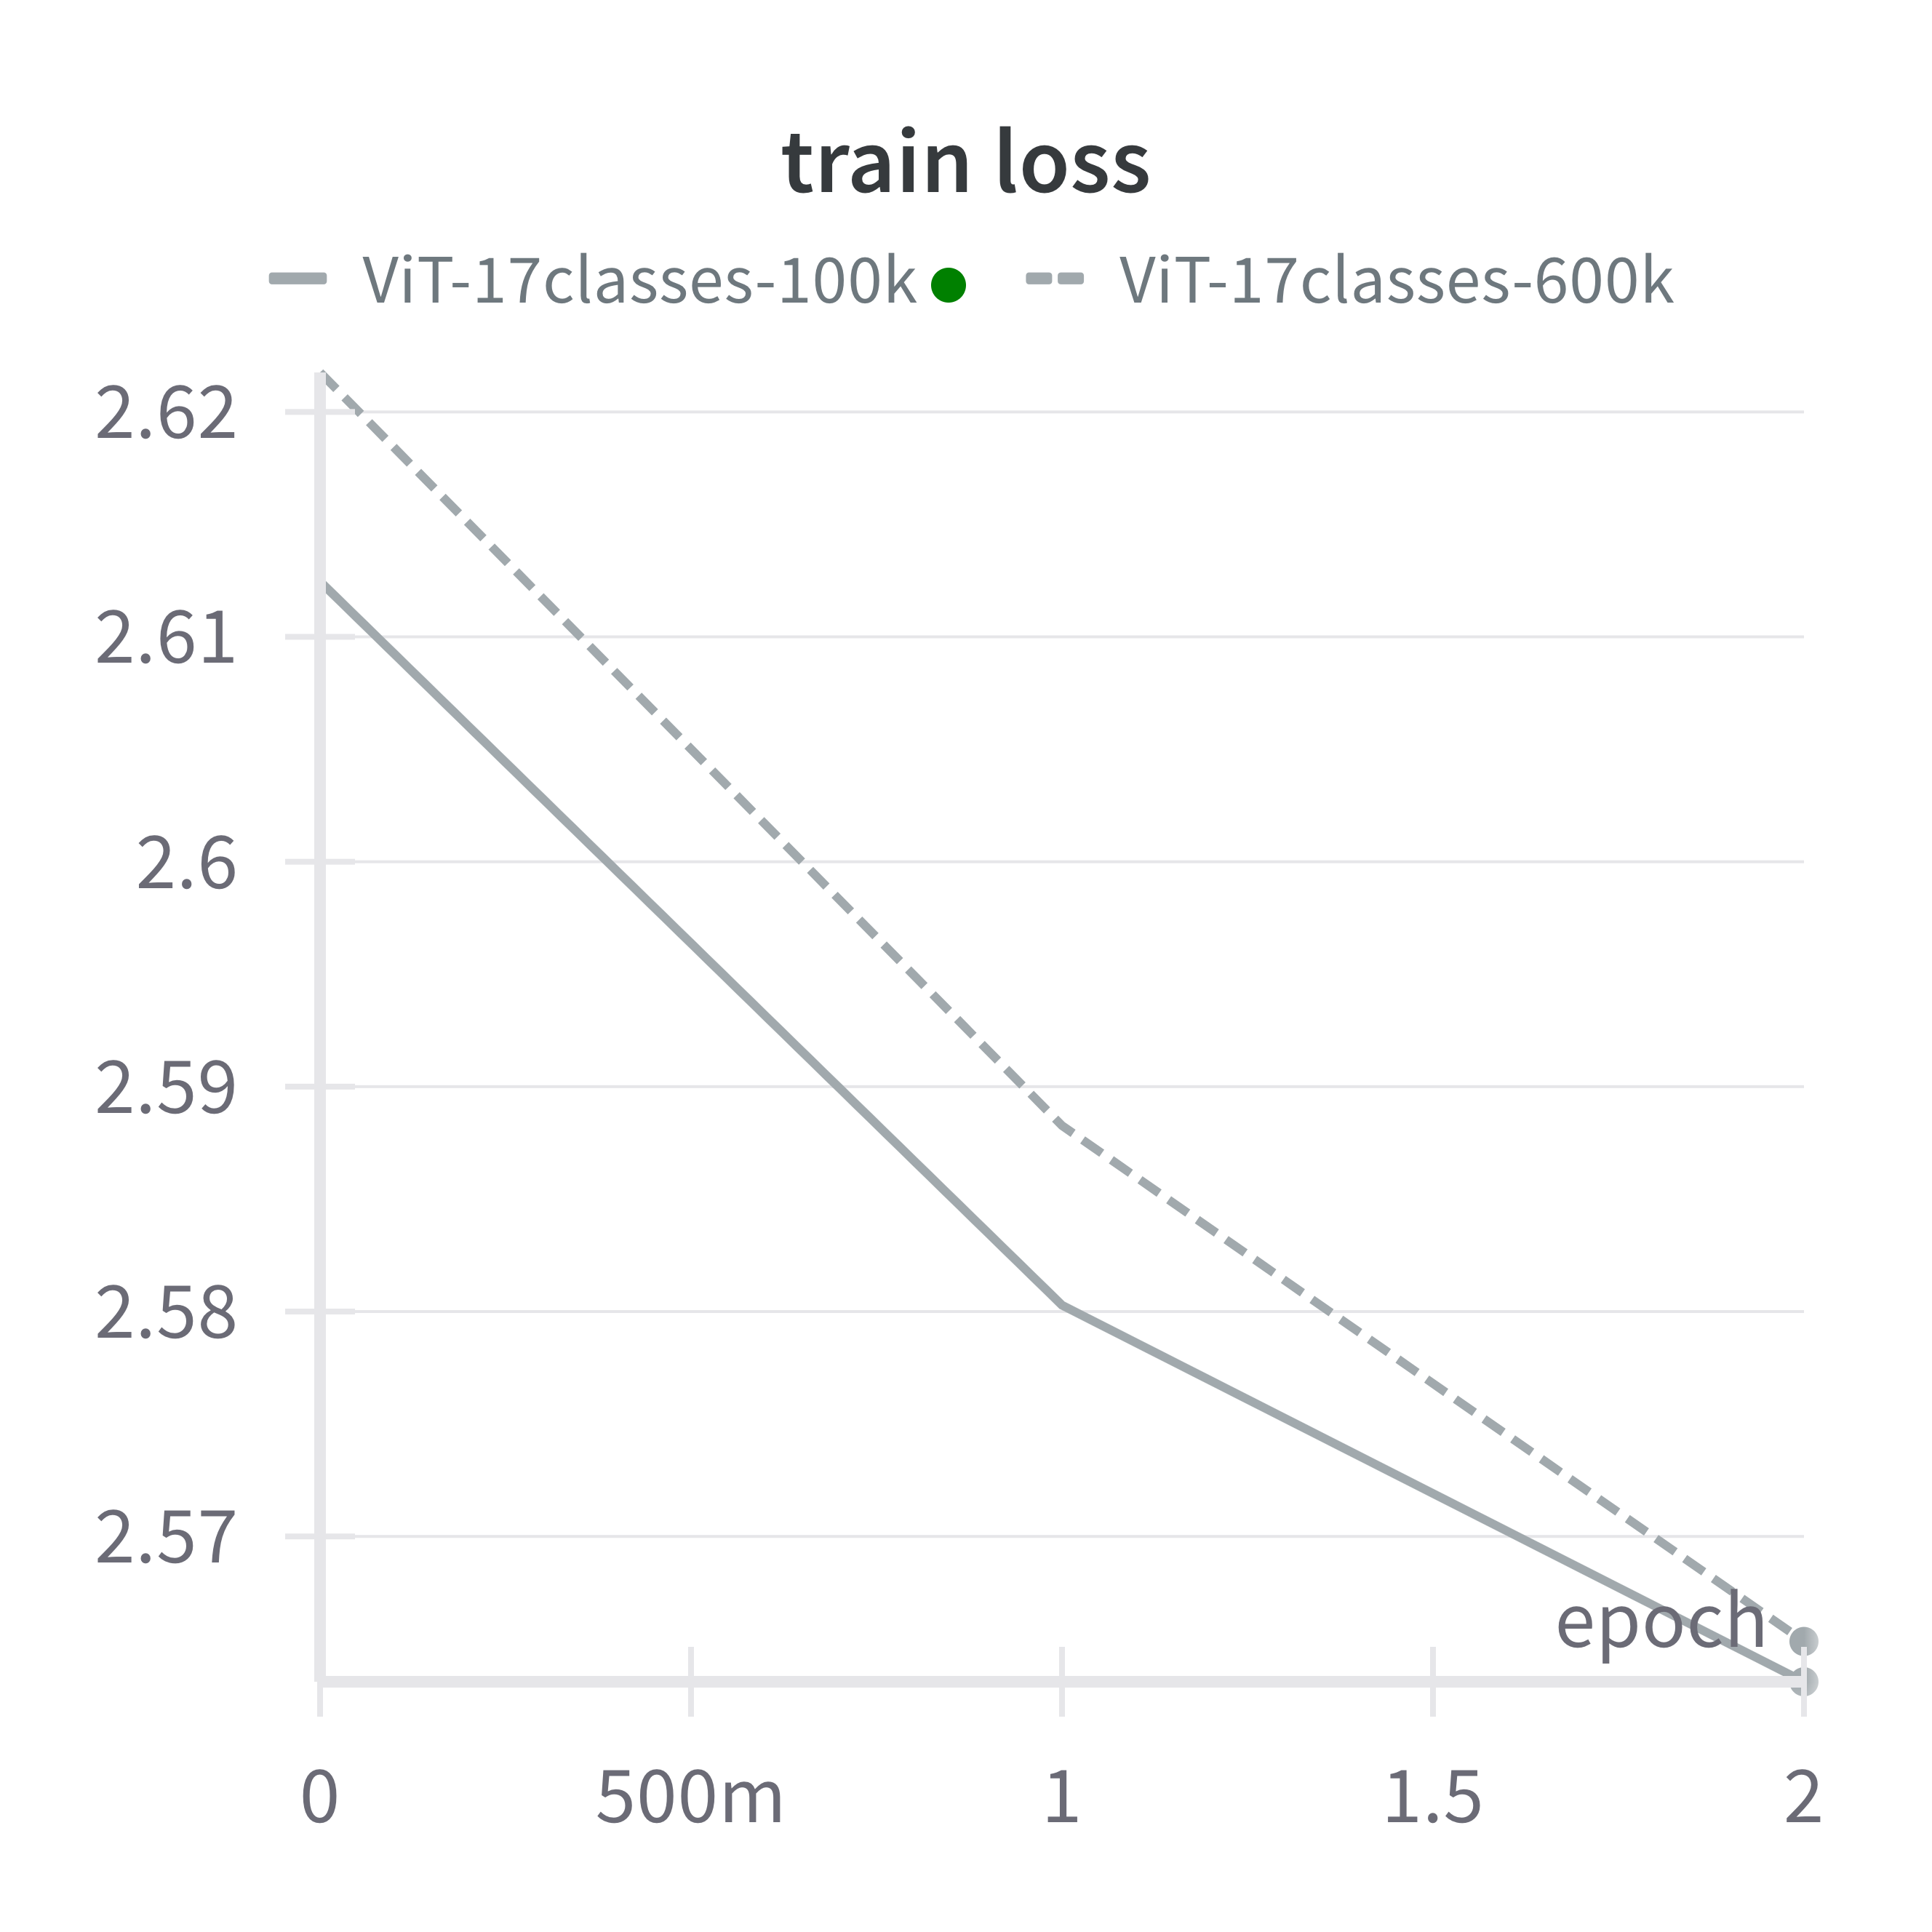
\includegraphics[width = 0.99 \textwidth]{images/17classes_vit_train.png}
        \caption{Train Loss}
    \end{subfigure}
    \begin{subfigure}{0.35 \textwidth}
        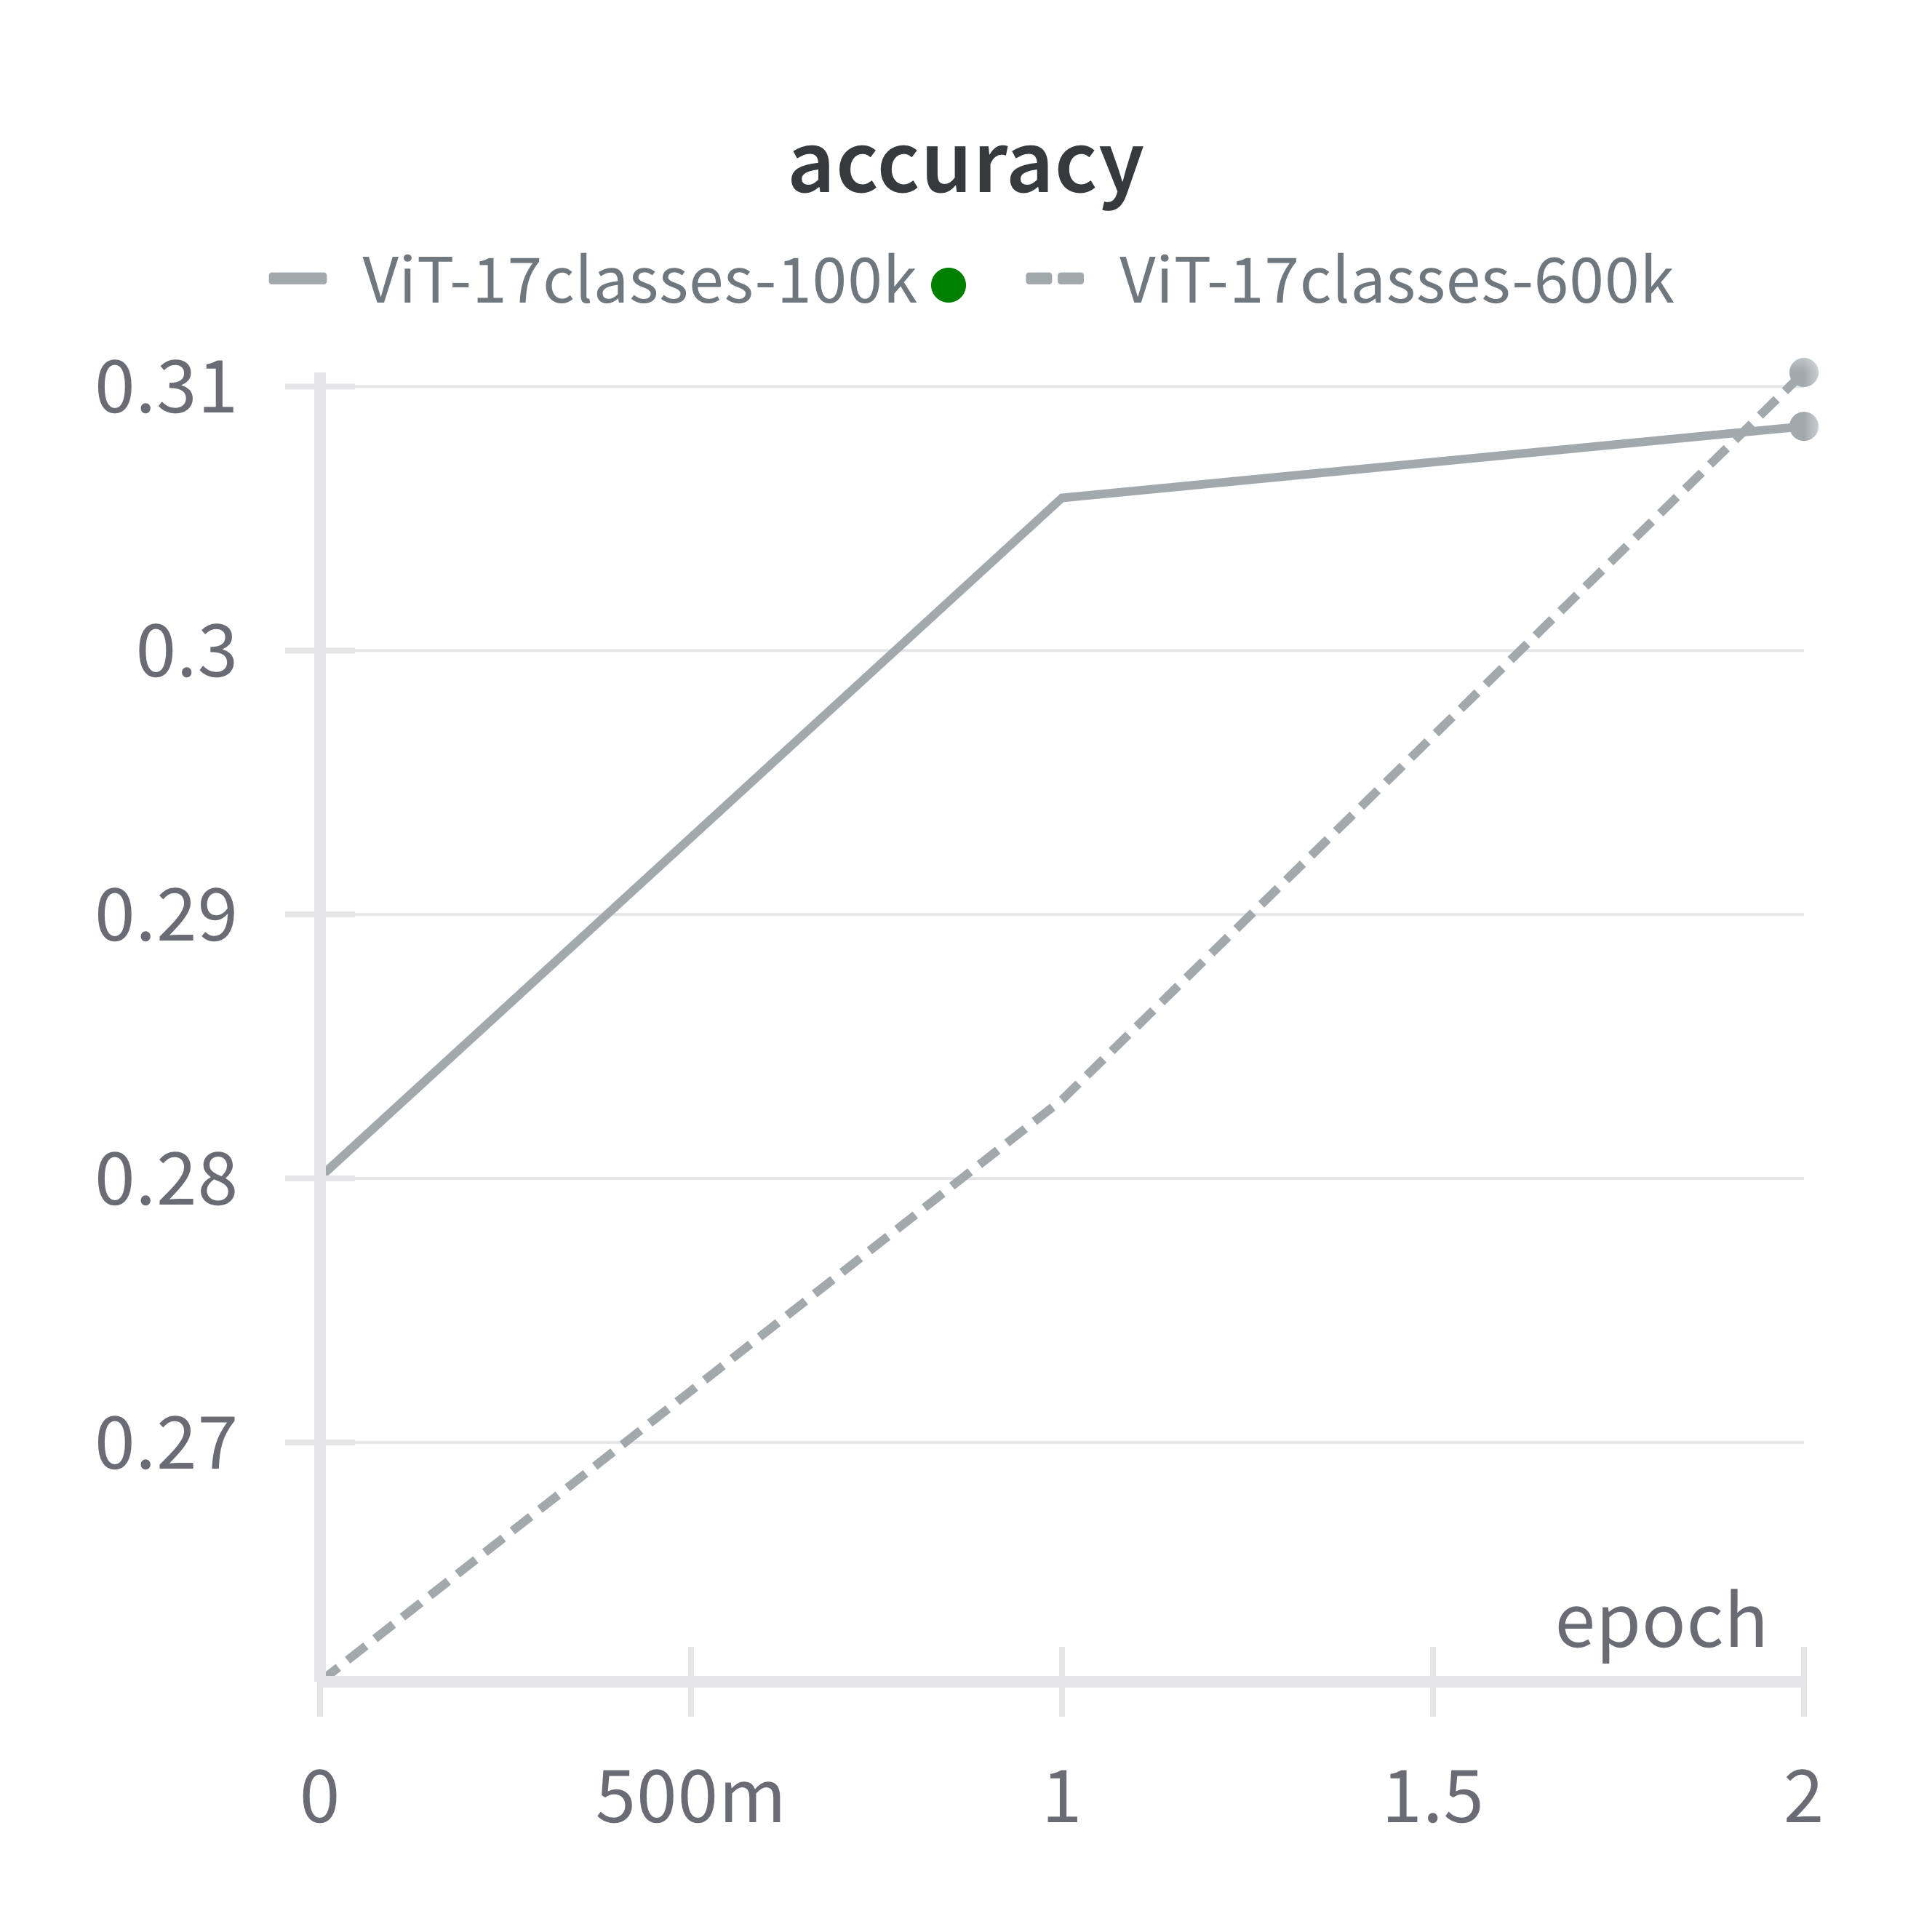
\includegraphics[width = 0.99 \textwidth]{images/17classes_vit_accuracy.png}
        \caption{Accuracy}
    \end{subfigure}
    
    \caption{Performances of two versions of the visual transformer on the condensed version of the \textit{Places} dataset}
    \label{fig:17_vit}
\end{figure}

\subsection{Qualitative Results}\label{sec:qualitative}

\subsubsection{DenseNet}

In this section, the qualitative performances are analyzed on the entire Places dataset and its condensed version. To do so, it has been decided to use the DenseNet model since it is the one showing the best final accuracies. The goal is to show the model's ability to make accurate predictions and to understand the nature of its incorrect predictions.

\begin{figure}[H]
    \centering
    \begin{subfigure}{0.235 \textwidth}
        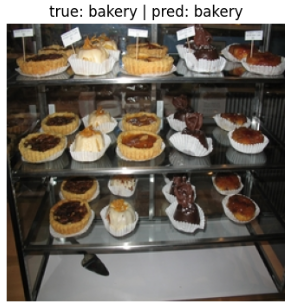
\includegraphics[width=\textwidth]{images/205_good_bakkery.png}
        \caption{Correct prediction}
    \end{subfigure}
    \begin{subfigure}{0.235 \textwidth}
        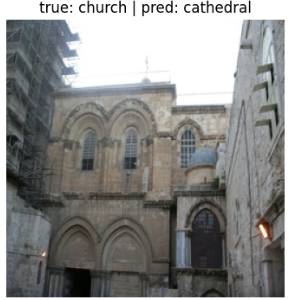
\includegraphics[width=\textwidth]{images/205_error_church.png}
        \caption{Wrong prediction}
    \end{subfigure}
    \caption{Predictions of the DenseNet on the full \textit{Places} dataset}
    \label{fig:205_quali}
\end{figure}

In the Places dataset, the DenseNet model shows some ability to perform, correctly classifying many complex scenes. For example, as shown in Fig. \ref{fig:205_quali}, the model successfully predicts that a bakery is a bakery. This highlights the model's ability to recognize the characteristics and contextual elements typical of a specific environment.

However, when the model makes errors, these predictions are often close to the correct label. Again in Fig. \ref{fig:205_quali}, the model predicts that a church is a cathedral. Although this is a misclassification, the object still belongs to the same general category of religious buildings, indicating that the model has a good understanding of the context of the scene, even if it doesn't always assign the correct label.

\begin{figure}[H]
    \centering
    \begin{subfigure}{0.235 \textwidth}
        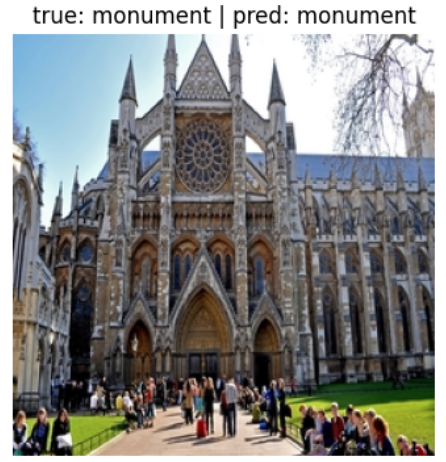
\includegraphics[width=\textwidth]{images/17_good_monument.png}
        \caption{Correct prediction}
    \end{subfigure}
    \begin{subfigure}{0.235 \textwidth}
        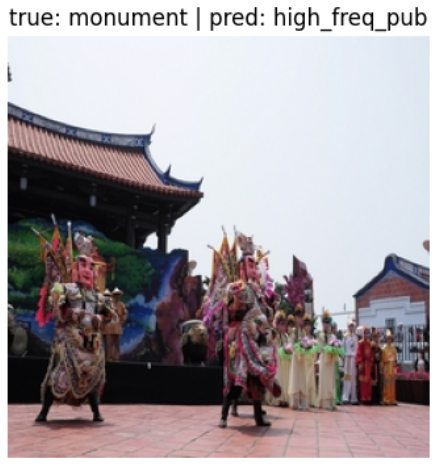
\includegraphics[width=\textwidth]{images/17_error_monument.png}
        \caption{Wrong prediction}
    \end{subfigure}
    \caption{Predictions of the DenseNet on the condensed version of the \textit{Places} dataset}
    \label{fig:17_quali}
\end{figure}

The problem of fine-grained misclassification has been tackled by using the condensed version of the Places dataset. This adjustment was intended to improve model performance by focusing on broader scene categories more relevant to real-world applications.

The results obtained on the condensed dataset confirm this hypothesis. In Fig. \ref{fig:17_quali}, the DenseNet model accurately predicts that a monument is a monument, demonstrating its improved ability to generalize over broader categories. This suggests that the model can now more effectively distinguish between significantly different environments, which is crucial for practical applications such as robotic navigation.

Nevertheless, some classification errors persist. For example, again in Fig. \ref{fig:17_quali}, the model predicts a busy public place instead of a monument. The image in question shows a monument surrounded by many people, leading the model to focus on the crowd rather than the monument itself. This type of error shows that even if the model's predictions are more in tune with the actual scene, it can still be misled by prominent elements that dominate the visual input.

\subsubsection{Visual Transformer}

To demonstrate that the Vision Transformer (ViT) is correctly implemented and its mechanisms are functioning, despite the suboptimal results on Places205, we generated "attention maps." By doing so, we aim to gain a deeper understanding of the inner workings of the transformer. We utilized the trained ViT model on the Intel dataset, as it achieved the highest accuracy in our predictions. By extracting the last block of this model, we accessed the multi-head attention maps corresponding to these predictions. From these maps, we computed the class attention map, which illustrates the weights associated with different regions of the image. This approach allows us to visualize where the ViT focuses its attention across various images.

\begin{figure}[H]
    \centering
    \begin{subfigure}{0.235 \textwidth}
        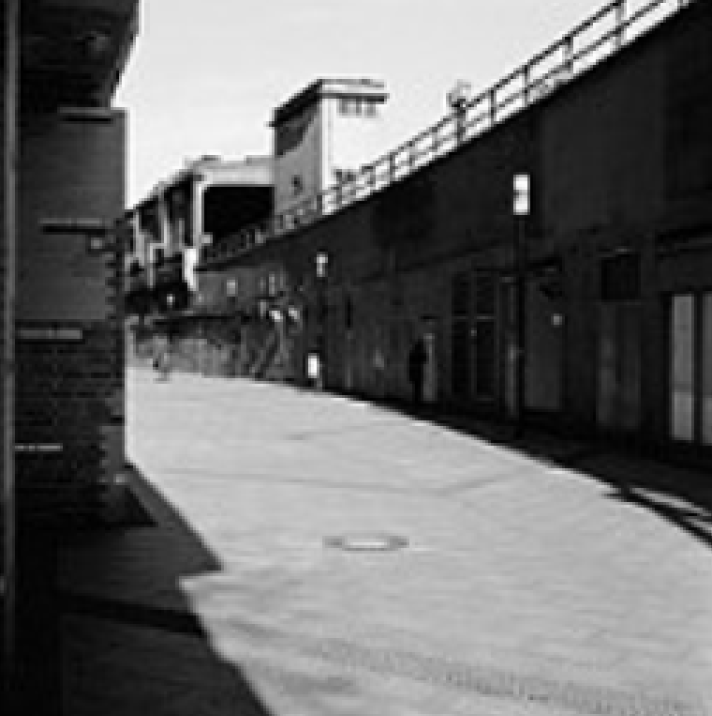
\includegraphics[width=\textwidth]{images/img_attn_street.png}
        \caption{Input image}
    \end{subfigure}
    \begin{subfigure}{0.235 \textwidth}
        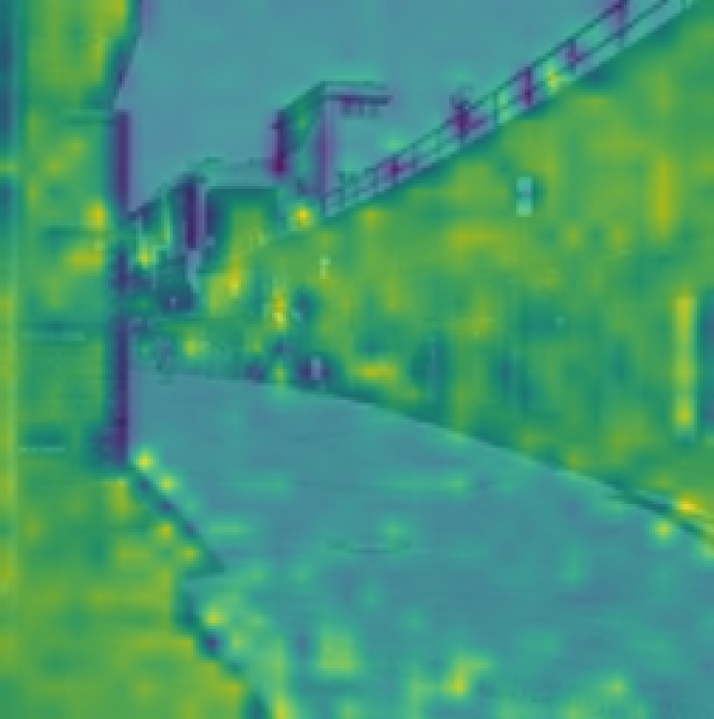
\includegraphics[width=\textwidth]{images/map_attn_street.png}
        \caption{Attention map}
    \end{subfigure}
    \caption{Attention map for the \textit{street} class}
    \label{fig:attent_map1}
\end{figure}
\begin{figure}[H]
    \centering
    \begin{subfigure}{0.235 \textwidth}
        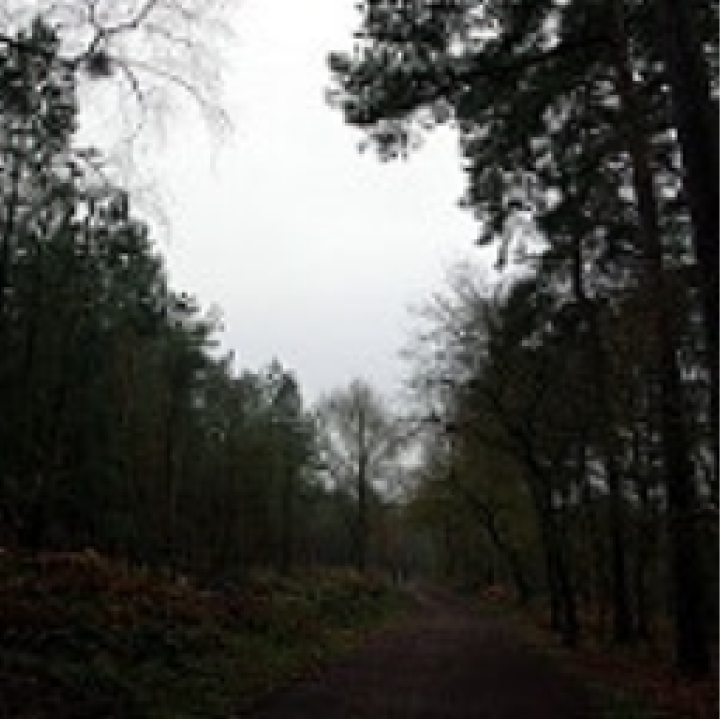
\includegraphics[width=\textwidth]{images/img_attn_forest.png}
        \caption{Input image}
    \end{subfigure}
    \begin{subfigure}{0.235 \textwidth}
        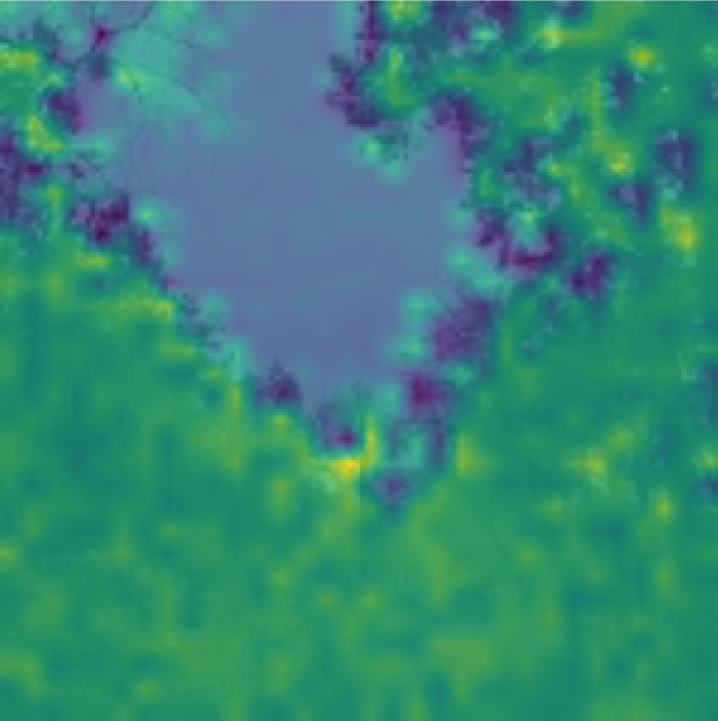
\includegraphics[width=\textwidth]{images/map_attn_forest.png}
        \caption{Attention map}
    \end{subfigure}
    \caption{Attention map for the \textit{forest} class}
    \label{fig:attent_map2}
\end{figure}

\begin{figure}[H]
    \centering
    \begin{subfigure}{0.235 \textwidth}
        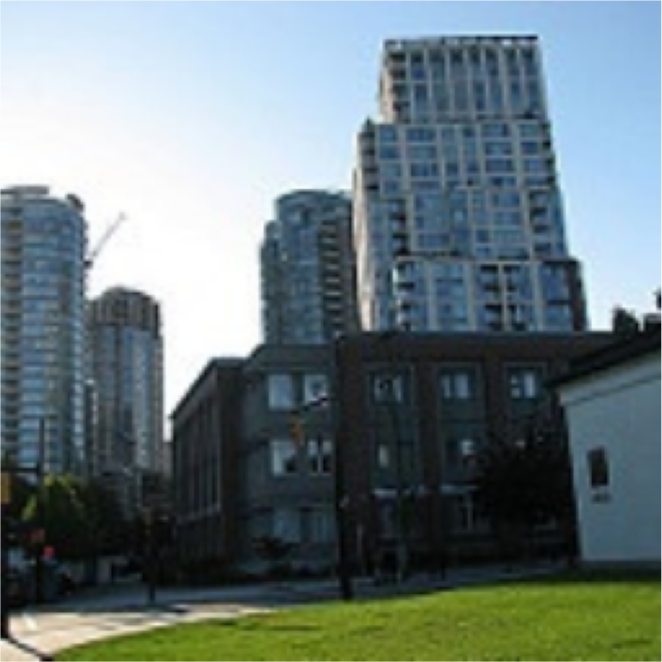
\includegraphics[width=\textwidth]{images/img_attn_build.png}
        \caption{Input image}
    \end{subfigure}
    \begin{subfigure}{0.235 \textwidth}
        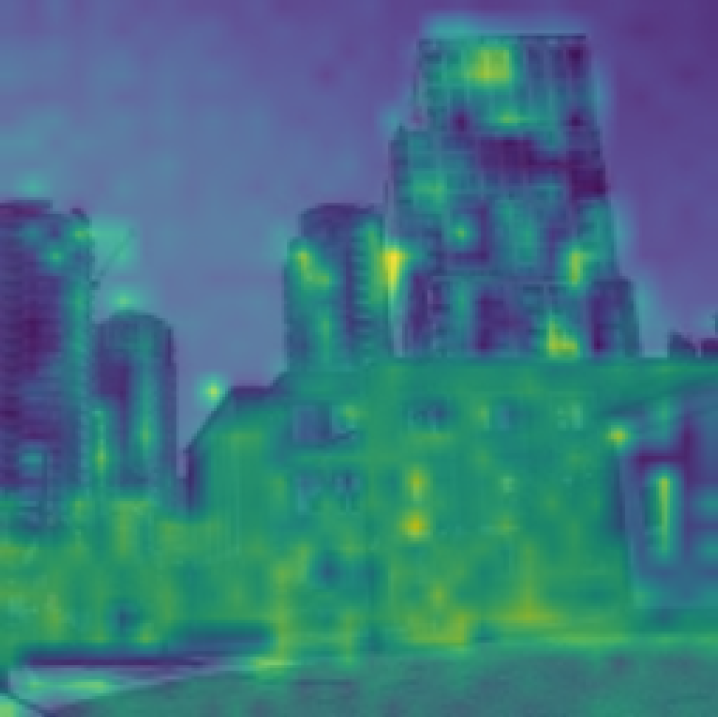
\includegraphics[width=\textwidth]{images/map_attn_build.png}
        \caption{Attention map}
    \end{subfigure}
    \caption{Attention map for the \textit{building} class}
    \label{fig:attent_map3}
\end{figure}

Like observed on Figure \ref{fig:attent_map1} /  \ref{fig:attent_map2} / \ref{fig:attent_map3}, the yellow tints indicates where the model has concentrate its attention and contrary to the blue ones. This mechanism enable ViT to focus on the most important parts of the input, capture context-specific information, more effectively than convolutional layers alone, to improve prediction accuracy.

\section{Discussion}

As a first final word, the significance of thoroughly understanding the dataset cannot be overstated. Initially, a cursory examination of the dataset was conducted at the onset of the project. However, upon constructing, training, and evaluating the models, a deeper exploration was undertaken, revealing that the "\textit{Places}" dataset comprises numerous classes that are closely related, as illustrated in Section \ref{sec:qualitative}. Therefore, what will remain is the importance of the research phase and the careful selection of the dataset. Understanding the intricacies of the data ensures more informed model development and ultimately leads to more accurate and meaningful results.\\

Building upon this problem, another valuable conclusion is the interest of dataset relabeling. By performing a straightforward operation —constructing a dictionary that maps each original class to a user-defined class— one can tailor the dataset to suit specific requirements, eliminate potential shortcomings, and enhance model performance while retaining the same architecture. This process allows for greater customization and optimization of the dataset to better align with the objectives of the project.\\

In conclusion, due to constraints in computing resources, the analysis could not be fully pursued, particularly for resource-intensive models like ResNet and the Visual Transformer. Additionally, all models were implemented using their lighter versions to mitigate these limitations. Therefore, increasing available computing resources could have potentially resulted in significantly improved performances. However, to determine the "best" architecture within the context of limited GPU availability for this application, ResNet emerges as the preferred model, since it would have led to the best performances with few additional training time. 


% ==============================================================================

\bibliographystyle{unsrt}
\bibliography{bibliography.bib}

\end{document}

